\chapter{Anwendungsbeispiel auf simulierte Daten}
\label{chap:4}

In diesem Kapitel betrachten wir die Leistung des hier vorgestellten Neuronale-Netze-Regressionsschätzers bei endlicher Stichprobengröße auf simulierte Daten in $Python$.

Die simulierten Daten welchen wir verwenden werden, sehen wie gefolgt aus:
Wir wählen $X$ gleichverteilt auf $[-2, 2]^d$, wobei $d$ die Dimension des Inputs ist, zudem wählen wir $\epsilon$ als standardnormalverteilt und unabhängig von $X$ und wir definieren $Y$ durch:
$$Y = m_j(X) + \sigma \cdot \lambda_j \cdot \epsilon,$$ 
mit $m_j \colon [-2, 2]^d \to \R \quad (j \in \{1, 2\})$ wie unten definiert, $\lambda_j > 0$ als Skalierungsfaktor welcher wie unten definiert wird und einen Rauschfaktor $\sigma = 0.05.$ Als Regressionsfunktionen verwenden wir die Funktionen:
$$ m_1(x) =  \sin\big(0.2 \cdot x^2\big) + \exp(0.5 \cdot x) + x^3$$
und
$$ m_2(x_0, x_1) = \sin\big(\sqrt[2]{x_0^2 + x_1^2}\big).$$
Wir wählen $\lambda_j$ als Interquartilsabstand einer Stichprobe von $m(X)$ der Größe $N = 800$. Mit diesen Daten lässt sich nun auch $Y$ darstellen.

Um die Leistung unseres neuronalen Netze Regressionsschätzers zu überprüfen, haben wir erstmals $m_1$ und $m_2$ und die jeweilige Schätzung durch unseren Neuronale-Netze-Regressionsschätzer für $\sigma = 0.05$ zeichnen lassen. 
Man erkennt dass der Schätzer eine sehr gute Approximation der Funktion liefert, aber um genauer beurteilen zu können wie gut die Schätzung wirklich ist und wie gut unser Schätzer im Vergleich zu anderen Schätzern abschneidet betrachten wir in Tabelle ... den Interquartilsabstand und den Median der skalierten $L_2$-Fehler der einzelnen Schätzer. 

Unser vorgehen zum Vergleich der drei hier betrachteten Regressionsschätzern gestaltet sich wie gefolgt:
Wir bestimmen erst den $L_2$-Fehler der einzelnen Schätzer approximativ durch den empirisch arithmetischen $L_2$-Fehler $\epsilon_{L_2,N}$ auf einer unabhängigen Stichprobe von $X$ der Größe $N = 1000$. 

Da wir unsere Regressionsfunktionen kennen und der Fehler stark vom Verhalten der korrekten Funktion von $m_j$ abhängt, betrachten wir den empirischen $L_2$-Fehler im Verhältnis zum einfachsten Schätzer von $m_j$, einer konstanten Funktion. Der Wert dieses \textit{konstanten} Schätzers bestimmen wir in dem wir das empirische Mittel der beobachtete Daten $Y$ nehmen. Wir erhalten damit einen skaliertes Fehlermaß $\epsilon_{L_2,N}(m_{n,i})/\bar{\epsilon}_{L_2,N}(avg)$ mit $\bar{\epsilon}_{L_2,N}(avg)$ als Median von $50$ unabhängigen Realisierungen von $\epsilon_{L_2,N}$. 

Wir bestimmten $\epsilon_{L_2,N}(\cdot)$ als empirisches Mittel von $25$ quadratischen Fehlern der Schätzung des konstanten Schätzers. Dieses skalierte Fehlermaß ist so zu deuten, dass ein großer Fehler durch einen der drei Regressionsschätzer im Falle dass der Fehler des konstanten Schätzers klein ist, auf eine noch schlechtere Performance hindeutet. Der Fehler $\epsilon_{L_2,N}(m_{n,i})$ wird also durch $\bar{\epsilon}_{L_2,N}(avg)$ gewichtet.

Die resultierenden skalierten Fehler hängen noch von der Stichprobe von $(X, Y)$ ab und um diese Werte besser vergleichen zu können, führen wir die Fehlerberechnung jeweils $50$ mal durch und geben dann den Median und Interquartilsabstand für die Schätzung der betrachteten Regressionsschätzer aus.
Wir teilen für jeden Schätzer die Stichprobe auf in ein \textit{learning sample} der Größe $n_l = 0.8 \cdot N$ und in ein \textit{testing sample} der Größe $n_t = 0.2 \cdot N$. Wir bestimmen den Schätzer für alle Parameterwerte mit dem learning sample und bestimmen das korrespondiere $L_2$-Risiko auf dem testing sample und wählen dann die Parameter die zu einem minimalen empirischen $L_2$-Risiko auf dem testing sample führen.

Unser erster Schätzer \textit{fc\_neural\_1\_estimate} ist ein fully connected neuronales Netz mit einer verborgenen Schicht. Dieser Schätzer hat eine feste Anzahl an Neuronen die wir aus der Menge $\{5, 10, 25, 50, 75\}$ auswählen die bei der Simulation zu einem minimalen empirischen $L_2$-Risiko führt.

Unser zweiter Schätzer \textit{nearest\_neighbor\_estimate} ist ein Nächste-Nachbar Schätzer bei der die Anzahl an nächsten Nachbarn aus der Menge $\{1, 2, 3\} \cup \{4, 8, 12, 16, \dots, 4 \cdot \lfloor\frac{n_l}{4}\rfloor\}$ ausgewählt wird.

Unser letzter Schätzer ist der hier vorgestellte Neuronale-Netze-Regressionsschätzer den wir mit \textit{new\_neural\_network\_estimate} bezeichnen. Hier haben wir die Parameter je nachdem welche Regressionsfunktion wir betrachtet haben entsprechend angepasst. Da wir zum Beispiel den Grad der zu schätzenden Funktion kennen und dies bei unserem Schätzer berücksichtigen können.
%
%\begin{figure}
%    \begin{subfigure}[b]{0.5\textwidth}
%        \centering
%        \scalebox{0.9}{
%          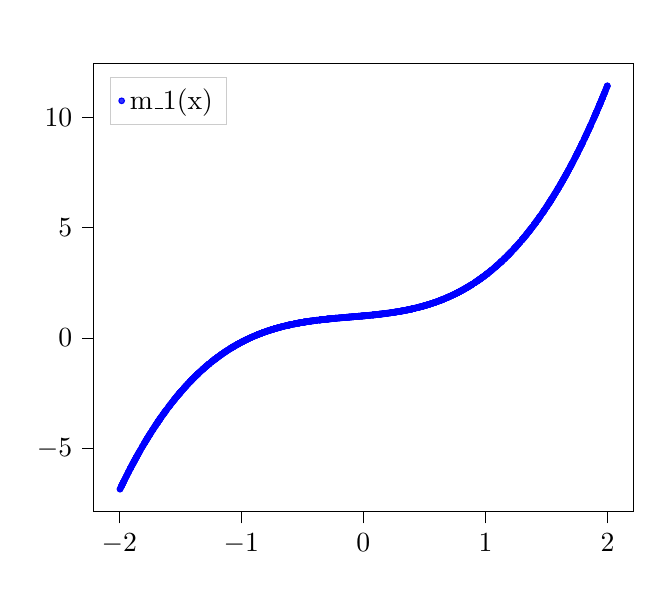
\begin{tikzpicture}
\begin{axis}[%
scatter/classes={%
a={mark=o,draw=black}},
legend style={fill opacity=0.8, draw opacity=1, text opacity=1, at={(0.03,0.97)}, anchor=north west, draw=white!80!black},
tick align=outside,
tick pos=left,
title={\quad},
x grid style={white!69.0196078431373!black},
xlabel={ },
xmin=-2.20852591900454, xmax=2.21306049239568,
xtick style={color=black},
y grid style={white!69.0196078431373!black},
ylabel={ },
ymin=-7.86405361849716, ymax=12.4391808546764,
ytick style={color=black}
]
\addplot[blue, mark=*,only marks,mark size=1]%
table{
x y 
1.98342671961567 11.2067083316341
-0.164883410431491 0.921819789666956
1.40142299960581 5.15033590554207
1.47929179834368 5.7561559124411
1.19715514411127 3.81799531027161
-1.05745151470862 -0.371309570367478
-0.696648319326161 0.464684877420012
1.82247761300943 9.15712037755566
1.33480759235371 4.67626070341997
0.862438587068488 2.32882713322422
-1.16503690445439 -0.754686954628516
0.417168238066338 1.33933090794867
1.15596892097842 3.59120483869643
0.850205757253619 2.28838577184768
-1.30994868597998 -1.39187573215822
-1.55346692657437 -2.82488317686155
1.61669575447566 6.96902026146192
0.500046589667835 1.45907874969249
1.28496886028727 4.34712794233107
-1.20227096727067 -0.904559178268851
0.366681884355046 1.27741420051878
0.818260589820523 2.18688479377424
-1.23845976488916 -1.05920098696907
0.697189507824902 1.8530215419852
1.93926361424016 10.6132554825254
1.04107639834298 3.02636787410901
-0.22353824693392 0.893074337960662
0.668246244317835 1.78431442012492
0.151928097424038 1.08704702436641
-1.07641959705448 -0.433765220730816
1.44298781246897 5.46662361852968
-0.284110387060426 0.860783387392703
-0.44017790192429 0.755901668314636
0.352464522063814 1.26134584362801
1.18574235128237 3.75381711403657
1.66572862979816 7.4485981217319
-1.77196434008901 -4.56390224034042
-1.42077197081339 -1.98366518029347
1.90156609340709 10.1254900733363
-0.399226079743066 0.787289288568677
-0.502642406493864 0.701288589370527
0.570484726981828 1.58079483029362
-0.626439688866295 0.563662303293445
0.646913187691053 1.73622883021686
-1.70011590874738 -3.94019890361793
0.188560902818183 1.11268318790154
0.613581309391728 1.66528403436379
1.53866334933713 6.25708686606659
-1.90745710621872 -5.88963818524853
0.41517370699518 1.33673477925145
0.327838052279217 1.23484812561957
1.73772873954887 8.19951335349887
-1.78984900196206 -4.72748294080677
1.52854808178337 6.16929527049623
0.00832534691972997 1.00418578874098
1.53059984449369 6.18702069900853
-1.45719188829622 -2.19959638868634
0.291257080120115 1.19843927737529
1.19523677300415 3.8071354073554
1.13842913470803 3.49861808490207
1.2366636859145 4.04822570623427
1.89871430519567 10.0892868982552
0.019953194670169 1.01011409945552
1.82122210851877 9.14233718077853
-0.298230517123074 0.852732115538147
0.382945539678767 1.29651503281945
1.08047569362621 3.20916222764976
-0.100962219519459 0.951781416117594
-0.409006788513409 0.780081708579802
1.41020530945337 5.21583204082174
-0.862424320245129 0.156477928786038
-1.98328806650409 -6.72214450231026
-0.696177128652387 0.465406125702621
-0.0933688730806197 0.955318102465428
1.94870249960763 10.73808188061
-0.936123458958722 -0.01976601438959
-1.58312442994531 -3.03409351460663
1.4664267507308 5.65211917053288
1.57141891136512 6.54839610341355
-1.47051135974113 -2.28133185267719
0.874729152014026 2.37035416122943
1.03751084984896 3.01036865668898
1.48030997994332 5.76445750267437
-1.54541524782003 -2.76946312915615
0.552369097636586 1.54760978330716
-1.68042557562017 -3.77839948923686
-1.51061355679375 -2.53657210298722
-0.167528933067055 0.920559140081827
-0.787421015424107 0.310011987252715
1.6501030154187 7.29301335433562
-0.0814367755752747 0.960885772415491
0.0795951024473589 1.04237142562678
0.979738939834169 2.76334381388308
-0.380817770934829 0.800394418604914
0.400591024706831 1.31813698650762
-0.4141113404742 0.776250097560955
1.91403104307527 10.2848760382045
0.920870673865245 2.53445330225573
-1.30315603463426 -1.35866671389968
0.0275601242433647 1.01404829046996
-0.927503900072607 0.00222689952751143
0.0368974953304853 1.01894249538715
1.15977317392 3.61159817433105
0.514097432066963 1.4818167241679
1.17984224265819 3.72104216577677
1.58572120040197 6.6789936011996
-1.37713701802779 -1.73918304115634
-0.472661706237887 0.728589446354698
-1.95506901984573 -6.40446611244112
-1.1779484446276 -0.805616762687941
1.23713048801279 4.05102163809569
0.455615485804151 1.39192818075103
1.59249283776102 6.74155542309861
-0.503448403039978 0.700525301295737
-0.446140509435029 0.75105598593073
0.0961164638478107 1.05196738610277
1.85889095909979 9.59383788518873
0.961953261926548 2.69181699566452
-0.383322867187997 0.79864530138838
0.24213138507616 1.15461989372253
0.788212033700322 2.09669287956382
0.84070370731225 2.25757827157573
1.40004883629895 5.14015179344157
0.107393086597664 1.05870960384272
0.225480591396121 1.14097309250214
-1.67936142766505 -3.7697647231671
-0.0816940927046601 0.960765514872752
1.47773128825186 5.74345186910455
0.401713010033748 1.31954418061981
0.422412491054748 1.34621800253768
0.776700220186323 2.06346076723564
0.317989295994632 1.22470791713495
0.816536031039081 2.18157160974445
1.53962127691442 6.26545353631168
-1.29064269548569 -1.29838208894096
-1.47198666263898 -2.29047742640869
-1.18769903957274 -0.844807189958559
1.5617847179266 6.46159449041297
-0.137017676939132 0.934967618307204
0.10162263173636 1.05523925887493
1.42737547993898 5.34593888574134
-0.755076052164864 0.368829213132414
1.71133977541391 7.91773667028815
-0.4721794317973 0.729011711839228
1.89344301858784 10.0226243465763
0.867958702524959 2.34736672383903
-0.411724457536147 0.778047811177945
0.824378736637617 2.20587035898719
0.170515291427536 1.09977047759294
0.979189264724758 2.76110191698977
-0.897121719560843 0.0767896021307181
1.55034434863224 6.35973527019784
-1.67062801778883 -3.69932121498425
-1.24614106788035 -1.09319208537185
1.54412256063696 6.30489082553266
1.43769151607769 5.42542699235533
-1.6456012323085 -3.50158560570617
-0.635373759957425 0.551982650209956
0.0798070563154254 1.04249250741436
-2.21592582434482e-05 0.999988920530453
-1.56549856175875 -2.90878956620822
-1.85995182081513 -5.40180355705662
-0.744024022342477 0.387963590115266
1.95878262880175 10.8725914329787
1.52876440755115 6.17116216956417
0.252423090403078 1.16334903121843
-0.393738335259513 0.791257880640355
0.449465165244776 1.38318113689044
-1.68386371444268 -3.80637391755432
1.00910500968525 2.88606233001523
-1.12050763647973 -0.587298253264637
0.230997555210016 1.14543091365568
0.0349769356316969 1.01792975394193
-1.56076894216133 -2.87564939931168
-1.45121512537244 -2.16340493618994
-1.16545297771441 -0.756311132410629
-0.0191205019479455 0.990551431326679
-1.86008081192998 -5.4030939017934
-0.436428121653843 0.758911768315441
1.49957184981221 5.9233919160222
-1.44219942190571 -2.10937609184844
1.01529613831035 2.91268092874956
-1.50140183330494 -2.47671254155102
-0.732092139869074 0.408086177914741
-1.31471126281736 -1.41536454673876
-1.16144104543941 -0.740697216143942
-0.689196716081129 0.475997455288745
-0.217022486630988 0.896366930296396
1.62508170186513 7.04925029897457
-0.0406198149252917 0.980157921905294
1.63119848795736 7.1082339788836
0.261617455458398 1.1713441338436
-0.0226785485704886 0.988815972333353
1.93031313461916 10.4958902043135
0.10579027870623 1.05774135817833
-1.34359720927249 -1.56148709026429
1.08272594869317 3.21993898042956
-1.13811010512611 -0.651956813151084
0.157670660808171 1.09091781606985
0.693694852953544 1.84450954897994
-0.413991721747403 0.776340444640307
-0.3496582994086 0.821300655555392
-1.494906796828 -2.43494997466264
0.0812226478153182 1.04330249998073
-1.87946646412891 -5.59912494096078
0.135232078225477 1.07608502949923
-0.0314802740817721 0.984550095861464
-0.536661666154805 0.667662425434589
0.939570817014385 2.6047405093355
1.9606433016915 10.8975565658301
-1.31276353932712 -1.4057380074589
-1.30676601901061 -1.3762731425726
-0.303871457144716 0.849451172880855
-0.643511730589387 0.541119017871324
-0.527466345137777 0.677041842362992
-0.522841202805422 0.681676958703923
0.4944545179478 1.45023449606521
-1.70114092695177 -3.94872752787689
-1.17864666831437 -0.808402179553694
1.70768647325131 7.87932950534975
1.57303031948494 6.56300623145007
0.553581378198257 1.54978869652802
-1.49462820991928 -2.43316685250796
0.0532637575658805 1.02770819278823
-1.03292019870819 -0.293649505337755
-0.0539046615190384 0.973832153044759
-1.4019635634533 -1.87640980895707
0.867566356157913 2.34604301414628
-1.05398034586825 -0.360109127135227
-1.13058478157364 -0.624075386023385
0.588011197017629 1.61419683576319
0.883913094472204 2.40197685981143
1.7032464005838 7.83284702573416
0.723806315564655 1.91984629454512
1.35906175870283 4.84427052411395
-1.23544243096618 -1.04596172691295
-1.54329111912356 -2.75493982502582
1.16098779424438 3.61813290630781
-1.87095954053839 -5.51258428050454
-1.2782629197376 -1.23986916511837
-1.05654172495337 -0.368367143763051
1.24353360832467 4.08955390230973
1.19028282951638 3.7792262679224
-0.775725735545598 0.33177186288789
1.02057273878203 2.93557518071213
0.821921250495339 2.19821881120506
0.918229962933942 2.52470603700035
-0.984864184033527 -0.151361080185913
1.93401749117918 10.5443463915569
1.83315978839409 9.28363700124014
0.533232250852013 1.51399333097939
-0.722014352421549 0.424656658899597
0.481969685265481 1.43090303239757
1.17847167126153 3.71346785213066
-1.79048490297368 -4.73336148187232
-0.945697114342179 -0.0446368331238406
1.60064007186754 6.81744991856981
1.93687669965452 10.5818612825148
1.35197568049207 4.79464642514883
1.91147516287336 10.2520425549434
-0.00460781786329045 0.997702891593491
-1.39948950363334 -1.86251399232994
1.04873511695863 3.06103594471185
0.000913924775346242 1.00045723462595
-0.50513266090352 0.69892519214253
-1.26704247379017 -1.18779508918314
1.76648926011692 8.515401523615
0.157856915922508 1.09104424813471
1.40787527714754 5.19838618820376
-0.240710854768439 0.88424614078834
-1.50153204953699 -2.47755356296565
-1.98239180697612 -6.71190905798603
-0.274480732689117 0.866148734835799
-1.63517535024967 -3.42099958712273
0.960111664862905 2.68452965066336
-0.166975897002565 0.920822887277161
1.54394939093015 6.30336988746059
-1.48090289946801 -2.34614449639195
1.23336476648575 4.02851752917348
-0.400362192403418 0.786460973883875
-1.87413140169175 -5.54475667677901
0.336611711534724 1.24409863604828
1.18872743268058 3.77050370068962
-1.7294971642558 -4.18886360380201
1.45013892943371 5.52266642043676
0.0983398967377997 1.05328401410495
1.82859103308664 9.22936432902555
-0.251038744131117 0.878821858955889
0.0752656353562249 1.03990925556896
0.0812009707648484 1.04329007921359
1.94778947733205 10.7259599229546
1.44701878178583 5.49815477228648
-0.327412551641523 0.835331216623138
0.243300205866964 1.15559974805297
0.092634846159414 1.04991799090477
1.99004222629651 11.2976793178811
0.370987182526909 1.28239482533905
1.12746366204799 3.44192570040845
-0.88103525140069 0.11444499583188
-1.87311208155932 -5.53440536407914
1.53244608154239 6.2030062191922
-0.460133374851041 0.739391819239952
0.307337448869911 1.21402461928519
0.369331774016094 1.28047335921953
-0.234023743918722 0.887711030862566
1.04808634766716 3.05808318471249
-1.71866655486462 -4.09618344887114
-0.541554732849246 0.662580975842837
-1.48954836729529 -2.40077032291578
-0.0346183802921285 0.983037951949156
1.66262513718082 7.41748978740735
-0.0632924638352459 0.969396910959773
0.0976192149694759 1.05285658014762
1.64277341714372 7.22092429870893
-1.23064117143324 -1.02502582306785
-1.2119829712324 -0.945178959503772
1.82543703976219 9.19203877696444
-1.96283859036236 -6.49099090907211
-1.07753916455694 -0.437518252974556
0.401431131407247 1.3191902799471
1.11313051112005 3.36918797402718
-1.82353738645624 -5.04487061859584
-1.02282270803728 -0.262684033496767
1.34249571990793 4.72895418337375
-1.7423388101225 -4.30030535815532
0.574932133692535 1.58914867255579
0.356056594784311 1.26535121241934
1.85225865167069 9.5131424338517
-0.398757442351753 0.787630287557302
0.689987650483266 1.83554534383615
-0.293455390498176 0.855480226380854
-1.36443451041482 -1.67085494806716
1.35065286985791 4.78543213551069
1.01572198192603 2.91452148801636
-1.34644750916868 -1.57624963302143
0.934098979805452 2.58394372921836
-0.337375961698936 0.82913400048838
0.64371991587656 1.72921343065672
-1.12505418398717 -0.603812272410027
-0.0424605535851552 0.97927752676906
-1.03874715299427 -0.311782480194157
-0.934567390971795 -0.0157678258945499
1.06185524551419 3.1213904800115
-1.68614727733944 -3.82501880552636
-0.0939923135416958 0.955027594191503
0.186353265908155 1.1110726428412
-0.702833029741399 0.455143382722217
0.669467597030042 1.78713226709335
-0.989846282352082 -0.16552193374252
0.105206333004412 1.05738943070462
-0.327016013168481 0.835575044028545
0.687399875760051 1.82932776989665
1.84677034716651 9.4467555282193
1.08694083448046 3.24022372148457
1.91270842735118 10.2678755681039
-1.84876330693187 -5.29058235734343
0.140188037147681 1.07929462015681
0.340988226479485 1.24879088314535
1.63241684639954 7.12002930432158
-0.134435062793881 0.936176722358918
1.89935988024498 10.0974738907713
1.10456045506315 3.32642942521779
-0.669863931935491 0.504430082672366
1.20253788657643 3.848623510478
-0.476896000953684 0.72485957082047
-0.864160922436813 0.152624313681391
0.779743629721808 2.07217627840376
0.44847566998307 1.38178594372062
1.88317123466855 9.8936753259772
0.966481764673039 2.70983107632884
0.977908789987251 2.7558871775324
-1.52375847203518 -2.62327699740979
1.13406912530685 3.4759673999773
0.522353840992912 1.49552708713273
-1.06822671124227 -0.406527917387101
-0.114355250680581 0.945546284394021
1.89308302690468 10.0180838654405
0.845248577878253 2.27224791568968
0.122425695926454 1.06795770242727
0.127977871489443 1.071452329096
0.01625186865687 1.00821615648482
-1.08796984143618 -0.472845104422563
-0.320666677251147 0.839450527601591
0.334320179485394 1.24166256257872
-1.05886861846269 -0.375902385164731
-0.564026324025872 0.638414711051878
-1.59115775979802 -3.0921520343033
-0.624686875303529 0.565923843870914
0.0413789150922659 1.02131826057146
1.31657491972719 4.55336406862912
-0.726992150093075 0.416520105094092
0.0524606842524733 1.02727218818635
-0.492141039700758 0.71109076518107
0.978275827209485 2.75738082493985
1.14130644500639 3.51364516032462
0.0392796360480538 1.02020313016701
1.30721738204172 4.49141064784605
0.490133920204322 1.44348012355915
-0.706442978901193 0.4495096644889
-0.993964710262591 -0.177329563835979
0.943620152780988 2.62025423675144
-0.0932557921766692 0.955370798670078
1.6365425027311 7.16008680515812
0.973324880119798 2.73730832363678
-0.725054451856926 0.419698555277889
-1.96417313354495 -6.50592462133396
1.31324497867966 4.53123083543522
1.87324432504556 9.77024625410757
0.303189087378309 1.20994224416354
1.9389374422235 10.6089613728723
0.501357612206841 1.46116901188386
-1.720056540905 -4.1080112039577
1.31781128519504 4.56160630738453
0.0951516110926338 1.05139794858651
0.408192815810979 1.32774813968817
0.513811453765586 1.48134650425401
-1.23574332705072 -1.04727912774199
-1.45264147142963 -2.17201479615298
-0.227918340918484 0.890843932569515
0.768794189473504 2.04105392984846
-0.383261040749235 0.79868859764658
-1.52535647365474 -2.63392131109938
0.978901900798691 2.75993067808586
0.989417826238432 2.80315006002761
-1.36387886985462 -1.66789491236366
1.30076519383918 4.44913205476502
-0.61920844932297 0.572929632714456
1.33769433552972 4.69598515376487
-0.74829966725375 0.380618179060386
1.65991412952015 7.3903995937643
-1.54882463937474 -2.79285887150011
-1.89409203935268 -5.74981453952136
0.116957207902192 1.06455795146663
1.17623321690576 3.70112896015788
-1.35372154548933 -1.61420715774001
-1.88141472578473 -5.61905888338989
1.32924807506156 4.63847962469226
-1.77134487512033 -4.55829675676622
-0.128741369799476 0.938838418393211
0.51095333379939 1.4766641046124
-1.67747670266001 -3.75449901365524
1.29669044236686 4.42261577546358
1.34952912501012 4.77761666284377
1.33266062176777 4.66163835456556
1.12465453846378 3.42754849841394
0.4823513930431 1.43148567258717
1.56244015327284 6.46747005636869
0.11081670699023 1.06078907799291
1.47420921577403 5.71486476538048
-1.40118206014657 -1.87201510170116
0.634664924286693 1.70957467919594
-0.684074619393981 0.483658496059001
1.60007325210646 6.81214767306192
0.871416435428499 2.35907231047904
-0.983390175523971 -0.147197135538043
-0.681323886845001 0.487734387895415
-1.26150283611157 -1.16241909746674
1.67379753998392 7.52995968901337
-0.987930545268803 -0.160060852020812
0.454921140058064 1.39093417506421
1.51394338581359 6.04432436735546
-0.804954691722807 0.276317438492785
-0.830724433208845 0.224398470191638
0.335858029439155 1.24329584466934
-0.159847298344431 0.924212755588489
0.0812119985668653 1.04329639798377
-0.117494185355901 0.944084196411911
0.497555841122187 1.45512515695177
0.640924836877307 1.72311134065059
-0.123471924446762 0.941297774124052
1.15598732778889 3.59130324256049
-1.27272624906405 -1.21406008321854
-0.76949998857843 0.343125991938706
1.4162089827075 5.26101451251004
-1.91041766129389 -5.92088694414514
1.99504962001563 11.3668989718006
-1.00490416987749 -0.209143338340367
-1.14258809682261 -0.668718416842979
1.18209823855401 3.73354181514181
0.128884868780194 1.07202738126087
-1.94570137893154 -6.30108914105676
0.27471991687839 1.18306806252273
-1.72671969673579 -4.16498229116897
0.187211122317864 1.11169743641647
0.48198115722144 1.43092053557093
-1.98132421803257 -6.69972954213555
0.758502825129475 2.01238871783111
1.34931125357486 4.77610269536153
0.245180659219023 1.15718232866859
-0.276183458320058 0.865207129827379
1.39456510983045 5.09968311504284
-1.6804327463332 -3.77845771215393
-0.665754239595305 0.510306575023814
0.76684140612743 2.03557122891776
1.09948744175177 3.30137507524853
-1.7534846008282 -4.39840634527731
-1.83044998652393 -5.11151071125484
1.37370201959309 4.94821688942207
-0.382340179934817 0.799332698920512
1.84016263074689 9.36729469457565
0.288068510119739 1.19542452478037
-0.114543656857639 0.945458542257138
0.206795309294432 1.1263285058384
-1.57769003775003 -2.99515593056534
-1.03763955741927 -0.308320801104982
-1.52268760032851 -2.61615653065817
1.11941760456987 3.4009040701208
-1.33311090638393 -1.50771004489711
0.128759478350397 1.07194781107472
-0.202242477740643 0.903731634603166
0.878360806223666 2.3827980126127
1.19855610565421 3.82594465441631
-0.95885680090605 -0.0795950750614648
1.9731762658412 11.0668248504742
-1.30507394687268 -1.36800862623331
-0.0157669575178914 0.992193314134026
1.88887607888191 9.96513724318019
-1.01174714032224 -0.229379091520865
-1.56039182316205 -2.87301570032441
-0.926950247777248 0.00362671646421875
1.64418618486032 7.23477519532048
-1.20043385996112 -0.896947485134618
-1.59792808416967 -3.14154749994605
1.69730156795686 7.77094735900795
0.575625029518244 1.59045760970327
1.4325210476095 5.38546272461785
-0.821655978972185 0.242999595633413
-0.810842030128184 0.264710330683507
-1.76436741471195 -4.49543613243629
-0.101373628416222 0.951589874479197
0.645687235329547 1.73352993640201
0.10576329327991 1.05772508508171
0.497152732945724 1.45448746150772
-1.20605108820682 -0.920293170938932
1.65818341412337 7.37314604751803
-1.87962426988887 -5.60073796632451
1.33566435853625 4.68210715495086
0.282054103858054 1.18980470698956
-1.26250466931175 -1.16699204691647
-1.67476380995526 -3.73258686461563
1.01967995195807 2.93168806191011
-1.67840964447672 -3.76205118380057
-1.50130451410046 -2.47608408679851
0.141109062399635 1.07989515924757
1.20995178365977 3.89118827835135
-0.531511081284835 0.6729432404821
-1.54006889061477 -2.73298567027789
1.66007705123738 7.39202540581725
1.38566787929341 5.03460666896519
1.42172807729341 5.30284416594051
1.19501735684592 3.80589515622314
-0.0613276058947694 0.970323119939249
0.588196574174466 1.61455706145536
-1.86528429810381 -5.45530051391384
0.327998076046251 1.23501500011517
1.94392556510098 10.6747725129444
0.391687289083808 1.30710792726173
0.953213581470196 2.6574299461252
-0.727575792369922 0.415559950077793
1.21439774087505 3.91692509422767
1.65999716563432 7.3912281841227
0.382087929756178 1.29548822962649
-0.16287160981814 0.92277676837371
-0.0542029915768536 0.973690800842405
-1.63260596193285 -3.40129984579709
1.12690113690572 3.43904191500925
-0.602201080415101 0.594083125950106
1.26792747852857 4.23945539583106
1.30847145779741 4.49966965275129
-0.718738337998323 0.429960531379342
-1.86119536711375 -5.4142508988663
-0.356727609725149 0.81669094026702
1.90459290272936 10.1640216503881
-1.44227588332194 -2.10983146250815
-0.391557970599605 0.792819909722158
0.631524958158446 1.70285186854789
-1.8673507757779 -5.47611714719273
1.42661454192866 5.34011495936151
0.170205151974584 1.09955348313825
-1.83568026427185 -5.16227865205378
1.2073940863486 3.87645422732492
0.706156293104354 1.87513804754791
-1.98203177551578 -6.70780014014512
1.36502793573962 4.88639889620432
0.399224089177922 1.31642786191096
-1.0253447363566 -0.270364174212614
1.50929202137678 6.00496342833847
-1.63337973901535 -3.40722582261244
0.16217533939344 1.09399145885371
-0.98542617423463 -0.152951737923894
1.5360467607192 6.23427976294006
-0.483081925171916 0.719337382260632
-1.58770633174206 -3.06713467478903
0.754998431678347 2.00275622643676
-0.315694310614774 0.842448548232049
0.80731770988626 2.15345551594596
-0.520999610898754 0.683507318681412
1.49195497855709 5.86011399750875
-1.10514956412394 -0.532465223812011
1.97857357935404 11.1403174392499
0.201904204556214 1.12260731318804
-1.48063273802369 -2.34444782161577
-1.74765842069912 -4.3469663733447
0.97582411111886 2.74742059343922
-1.94025775141107 -6.24148801641387
0.378690645694897 1.29144231745017
-0.675642050925532 0.496069283877749
-0.85135959252331 0.180704325857191
1.29651347872175 4.42146741003185
1.38442162021466 5.0255486562329
0.0993659004083431 1.05389365645253
0.322056803667919 1.22886488173402
-0.319240158445763 0.840313911505586
-0.584549292170264 0.615110609184494
-1.12598759652605 -0.60721864335168
1.41262589486618 5.2340088706993
0.646121632266878 1.73448545340135
1.78052185613418 8.67289265981815
0.0456857711294889 1.02361857502653
0.650561123062864 1.74430075452423
0.444925785300273 1.37680795769407
0.360910773533672 1.27082206027476
-0.00804773722748919 0.995996648292271
0.377237311240174 1.28972199915939
1.52091849859923 6.10374749026291
-0.0373496792893628 0.981725351704962
0.862206665085895 2.32805217881156
-0.507190355652468 0.696960910121683
-1.86205179057238 -5.42283330831689
-1.70459448861946 -3.97754027439972
-0.151804594967045 0.928017392461753
-1.68436080041345 -3.81042813744005
0.187659122172576 1.1120242490766
1.3554496588658 4.8189190431175
-0.487869327729311 0.715003204906045
0.842675192251204 2.26392694634303
-0.912200762028982 0.0403535280591013
-0.946369416514677 -0.0464010410197027
0.330462441073498 1.23759349000862
-0.0195847733926913 0.990324603273036
1.26237990986932 4.20493049782254
-0.675334511443002 0.496517206261075
-0.229399784212416 0.890086353839939
1.9604831935885 10.8954066810646
0.653098747548911 1.74995226855662
-1.99271462098377 -6.83038081816128
1.52604705488264 6.14774493496474
0.265785713873526 1.17503120638017
-0.162967637142707 0.922731122134607
-0.283790790788197 0.860963045149854
-1.36121907666447 -1.65375883389091
-1.31329929847602 -1.40838314891627
1.81527813187679 9.07259527626234
-0.442821583254181 0.753762240778201
-1.35568360263731 -1.62451551362428
-1.51220574381476 -2.54699354010741
-1.88865198249977 -5.69348252498278
-0.0584710604719203 0.971671561732019
0.381577876562059 1.29487859540097
-0.606990213147065 0.58821653307224
-0.749626560934504 0.378324034734459
0.00894689778701219 1.00450019527111
-0.134416985656438 0.936185181356841
0.947482538246278 2.63514997624858
0.652193660151404 1.74793312291132
-1.4971053276791 -2.44904543319222
1.73588142591092 8.17953815015466
1.82488208996298 9.18548319269702
-0.433621813289647 0.76114591416293
-1.85764198404764 -5.37872869313915
0.189957707840087 1.11370674618603
-0.0839730204312175 0.959700875691003
1.24728831958757 4.1123056418777
1.65468022478909 7.33832011275106
-0.586495676362482 0.612837325483901
1.79589799743536 8.84802129209566
0.428791423729258 1.35471550491822
-1.21645298698983 -0.964090333743602
1.5431165224241 6.29605904121035
0.178665194044994 1.10553169571189
-1.65418653612307 -3.5687317524992
1.59677966307949 6.78140367909103
0.933307944837329 2.58095305728585
-1.77917297787843 -4.62942925053352
-1.02449591391644 -0.267775315313738
0.586894557125167 1.61203007076959
-0.522527848756777 0.681989010527291
-0.839039065755164 0.207022944691082
-0.985881123675554 -0.154240675866536
-0.464749211709719 0.735452035855211
-1.64426334947883 -3.491186075905
0.467548491374151 1.40927248703334
1.92460116275829 10.4214987297265
-1.6443087962847 -3.49153905651549
-0.491293941305216 0.711870026008429
1.91222188641349 10.2616270266605
-0.62453546156841 0.566118745447308
0.300401507594917 1.20722329431868
-0.408259673873164 0.780638446049794
-0.386727514305038 0.796251031923926
-1.2807629327012 -1.25159562141562
-0.35007346853807 0.821032011779048
1.81278321825848 9.04344311739489
1.04336477412012 3.03668320841017
-1.32183939999296 -1.45083724437438
0.292077450222015 1.19921892546656
0.994071082116497 2.82251080980646
0.177466744750081 1.10467731384257
-0.505717794748531 0.698367674676974
-1.43761031855531 -2.08213415727262
-1.89149919300563 -5.7229237053933
1.28583777853235 4.35268374821217
-1.68115385495103 -3.7843153794068
-1.4142254050391 -1.94600789683803
1.52526984373002 6.14106061529525
0.612917731722653 1.6639222092179
-0.607365102169935 0.587754345462488
0.0446778208985652 1.02307869555183
-0.96209360813814 -0.0883318304875763
1.30375431185376 4.46867408429554
1.44134726467672 5.4538346503775
1.00844224545156 2.88322832443489
-1.59164327974008 -3.09568014470601
-1.93898777050765 -6.22763304253179
1.75462960692508 8.38402365592018
0.409361680989284 1.32924207079661
1.96570363363382 10.9656676715992
-1.89042953048247 -5.71185225186763
0.634605413505302 1.70944684791535
1.51117328592788 6.02085759885574
-0.336130600952831 0.829916161502131
-1.70081948401835 -3.94605184186047
-1.17900918117107 -0.809849619160207
-1.88055737118247 -5.61028146583971
1.7226892869659 8.03798589758147
-0.28444331034676 0.860596119807494
0.256235525537556 1.1666413705637
1.70534277107545 7.85476685433527
1.12385801800205 3.42348268523638
-1.47077804764093 -2.28298371381439
-1.61806822565318 -3.29102278955293
1.90294759424218 10.1430630966633
1.44451129494468 5.47852266160623
-1.01616478290891 -0.242580965266955
1.15493317240572 3.5856718757953
-1.40498242439259 -1.89343221858113
-0.452277827687501 0.745991134070497
-1.02618668656894 -0.272936092067389
0.16135892421457 1.0934319415492
-1.38881021937692 -1.80309489411771
0.83749527307802 2.24729452697683
-1.50103564033491 -2.4743482179168
-0.486808076009357 0.71596857791788
-0.538027218351843 0.666250669752277
1.9974166483278 11.3997283821791
0.0678536146367503 1.03574211366182
-0.0899177932002528 0.956926814390687
-0.427960738075485 0.765604944431546
1.60332836723081 6.84264236473997
-1.91821035570889 -6.00361962545922
-0.484358263630535 0.718187066115336
-1.14455694548876 -0.676128497006041
0.0304102520839233 1.01553439168116
-1.35890685005729 -1.64151467560062
-0.79930465921805 0.28731719612153
1.73862147320117 8.2091801257019
1.45803599732521 5.58511646755393
1.89547191274214 10.0482431762309
0.690931727750082 1.83782178852227
-0.621921289478656 0.569472296962388
-1.85804910216955 -5.38279143389878
-1.90519163173854 -5.86579373854702
-1.16833564944958 -0.767594943367109
-1.97462737655031 -6.62363958121218
-0.318014178865605 0.84105380251823
-1.6721081152242 -3.71120685604103
0.12506651417845 1.06961442749644
-0.598865775068001 0.598127669210699
1.77408588270415 8.60038455461797
-1.28722274061527 -1.28210603288769
1.97264479348539 11.0596075319345
-1.38334936445139 -1.77306192632327
-1.4234852858919 -1.99937517996845
0.68138823441224 1.81500941674427
1.04276100159047 3.03395800254456
0.363443058450483 1.2737027863533
-0.484681708491861 0.717894959660252
-0.42417904656689 0.768548456579527
-0.463869516349239 0.736206471705505
1.51603821310448 6.0621205930325
0.758851818256217 2.01335155326038
-0.361724413726992 0.813386601010214
1.9077891816332 10.2048298360685
-0.325593495457903 0.836447991161261
-1.4194697586773 -1.97614676213254
-1.98060600755018 -6.69154355462185
-0.74386957637504 0.388227584497721
0.0550760056004314 1.02869441717498
-1.07639607264541 -0.433686442070373
-1.98146995411248 -6.70139135895703
-0.614558293171367 0.578802301776621
0.580519533847571 1.59976104188703
0.85530197722539 2.30512646438327
1.16025561474269 3.61419236913617
-0.856557722320832 0.169393066404631
-1.15325753072591 -0.70917200147902
-0.239167870624584 0.885048828266123
-0.763721926225796 0.353522802407235
-0.977358490724609 -0.13027982803673
0.778036169125887 2.06728038238241
0.884340845547061 2.40346215552389
0.328138275778158 1.2351612579192
-1.55099225540116 -2.80778775223326
-1.03940188301237 -0.313832078552333
-1.72324163505083 -4.13518796186514
-1.84654800214979 -5.26872481567198
-1.43760044903241 -2.08207575751688
1.33241634702983 4.65997723453523
0.00470785624302161 1.00236123791202
-0.756956890576916 0.36552483747915
1.47817407575479 5.74705420485713
1.7488753934927 8.32084679314365
0.24029622852773 1.15308731260398
-0.229712543158756 0.889926204763276
0.936394382750414 2.5926445628988
-0.588247452495922 0.610781821734327
1.12089743121385 3.4084122555828
-1.68973056641353 -3.85438000159527
0.601490598378976 1.64077414366491
0.485060318584069 1.43563571921682
-0.743511201112161 0.388839796458524
-0.237997845978876 0.885656203601219
0.465159036576552 1.40575968640309
0.221364441760389 1.13768751303374
1.84453390617883 9.41980429808891
1.00647655101298 2.87484055951728
1.01000925130016 2.88993373969193
-1.87754777380837 -5.57953526649142
0.768807495091131 2.04109135728871
-0.126510324543307 0.939880107966774
1.59224876657191 6.73929233360148
-1.96901747277081 -6.56031066024765
-0.151585860600471 0.928120599126281
0.27514404486757 1.18345419050871
0.928969564002895 2.56462168594107
-1.13912071298838 -0.65572847467495
-1.3946007413604 -1.83520004087116
-1.53647125544187 -2.70858343004002
-0.853899259225281 0.175193415056966
-0.168066577292175 0.920302623347891
0.80680243856385 2.15189801728073
-0.568715904490896 0.633195480283646
1.90853719763859 10.214397764992
-0.788490064341025 0.30799463717303
0.442582735811799 1.37354566431466
0.459054233603626 1.39687552247798
0.39261749399079 1.30824877454604
-0.334717090759574 0.830801289010195
1.94086803536182 10.6343968181273
1.72074136428306 8.01724701749925
-0.292636510585159 0.855948854822363
-1.8825587450258 -5.63078399959954
-1.44751382991273 -2.14114206316334
-1.66380916147449 -3.64484099058998
0.401861302912721 1.31973046275312
0.623271629065938 1.68539340121019
-1.73144970591821 -4.20569915378075
-1.77371702050308 -4.57978392318897
0.955956320015098 2.66816793758185
-0.18897993598519 0.91023036546916
-1.6234885758441 -3.33190439423898
1.09818757474448 3.29498592215778
0.309124261139459 1.21579642671328
-0.0852514379276199 0.959103955205731
-1.20296402390791 -0.907436646342982
-0.270626161478439 0.868269331607198
0.580911905551383 1.60051121866171
1.89911009192989 10.0943055577833
-1.064461094195 -0.394142474879605
1.01285946066994 2.90217317390131
0.0402853617909917 1.0207368752534
-0.721932674649874 0.424789386080467
-1.66297073792276 -3.63817368047019
-1.81194227253934 -4.93425282463376
-0.65222601397195 0.529244626005021
-0.471450844379962 0.729648654986886
0.0370646534067927 1.01903079271421
-1.40749154055525 -1.90763621540311
0.695183252394338 1.84812752899872
-1.3887485131105 -1.80275420632957
1.85291059689277 9.52105182117024
-0.357923961782797 0.815903315065873
0.974884463317879 2.7436137850711
1.09839082028482 3.29598410091773
0.830736918330413 2.2258271038816
0.470309061762373 1.41335589628585
1.72836875306984 8.09869154159071
1.46857383792811 5.66937208921194
0.456457372499913 1.3931356304433
1.66877894800176 7.47927364775083
1.39834539959636 5.12755138331202
1.56275324449412 6.4702782522399
-0.325545359330059 0.836477482958752
1.85992830537649 9.60650597509558
-0.723639418786876 0.422010679340869
1.94494266655738 10.6882289495346
-0.603203955844345 0.592860405091233
1.7499954109815 8.33311478767895
-1.54049166796916 -2.73586090180703
0.259609595491829 1.16958206817038
-0.731632112601908 0.408851007811368
-0.0519325411599803 0.97476729017708
-1.72438866505661 -4.14500022640276
1.5064929250508 5.98137889887683
0.887629961378167 2.41492021599477
-1.11507085610526 -0.5677200891142
-0.917751339073211 0.0266596159564805
1.59838189136926 6.79634572283596
0.0866958965644469 1.04645605141118
0.511077028010305 1.47686610904852
1.18267057389016 3.73671928077183
-1.50837712909309 -2.52197132499597
-1.11106653271358 -0.553417700758948
1.81148448128094 9.02829616101279
1.50251810418365 5.94801949158777
0.814115306622483 2.17414199110334
0.790250422365434 2.10265274415143
1.63443981901696 7.13964875211235
-0.233454491645942 0.888004345247047
0.586663233387293 1.61158186572004
-0.0497866633920321 0.975786287788734
-1.61536089253957 -3.27070757076436
0.848178812923249 2.28176978444151
0.245000662573484 1.15703051541659
1.53488813686981 6.22420253630332
1.36834242044437 4.90994069397324
-0.704148960054754 0.453095256084725
0.00630860309351045 1.00316749235806
-1.40491432443655 -1.8930474153221
0.829387278753886 2.22157156070566
0.317830262660781 1.22454626287515
-1.90365540241397 -5.84965805885858
-1.62753556811879 -3.36260966263985
-1.07974178139327 -0.44492376214492
-0.0401652628917479 0.980375534538642
0.860426038380392 2.32211294404568
-1.97271544571729 -6.60201419432597
0.190591970662848 1.1141726925123
0.737104817700763 1.95457775769123
1.79080319347672 8.7896957865979
0.180385991615295 1.10676284928859
0.269402073604749 1.17826216971268
-1.21119745824843 -0.941869770922104
0.452501685883913 1.38748350398462
-0.672242667744425 0.501002119019167
-1.87624541070442 -5.56626179799371
0.697491518131789 1.85375997540669
-1.20317623202471 -0.908318352432709
1.03305973959424 2.99052061568452
1.93968190507009 10.6187642477155
-0.821861577213577 0.242581884621014
1.63669141219185 7.16153596429626
1.12811869078702 3.44528671234127
1.18993959765328 3.77729979941787
-0.25536082126297 0.876524214114186
-1.53401697010337 -2.69200261869658
-0.179743031420164 0.914703026826147
-1.02306687395788 -0.263426005993494
-1.74238098504039 -4.30067414845448
-0.468060562638022 0.732596940922769
-1.52858752321493 -2.65551241532027
-1.66643863626171 -3.66579564315443
-0.641421382308617 0.543930131873093
0.538245752971836 1.52265960139125
-0.955234916781065 -0.0698838993363239
1.80447172410411 8.94684189758768
-0.263185865738656 0.872320671481494
1.20310768144324 3.85187921672936
-0.759262351682819 0.361455230000449
-0.100655606763484 0.951924170797343
0.395716018306588 1.31206807179805
0.87211821829841 2.36145681851321
-1.15580354177307 -0.718933512086722
-1.46536166469255 -2.24955290054648
1.48295138677626 5.78604032278067
1.61459884644588 6.94907314634342
1.12568219517709 3.43280119124754
0.866338688902824 2.3419070079037
-1.88149196370742 -5.61985003530082
0.796995975427856 2.12253861289157
1.18993904227527 3.77729668298541
0.00326378068726907 1.00163538782081
0.99147879094986 2.81170713649919
-1.16854127436226 -0.768401909148824
-1.41411347488116 -1.94536708041133
-1.18129361556432 -0.818990900220248
1.75555598117783 8.39422907605019
1.4068679209575 5.19085919088058
-1.11794299148175 -0.578039886374277
1.35976299670166 4.84920562717139
-1.62864042117664 -3.37101946941616
0.837123791554514 2.24610769688773
1.90712812877881 10.1963798514224
-1.04264993613093 -0.3240363185946
-0.899533795903042 0.0710358364792234
0.131443054211328 1.07365571281068
1.58641001943151 6.68533601707391
0.133184681131325 1.07476973412852
-1.66808451108402 -3.67894626701431
0.958140299087838 2.67675334517056
-1.20071553721398 -0.898113080369225
-0.29853548062793 0.852555704806701
-1.59020194748787 -3.08521285924393
-1.14679993698604 -0.684600564244047
-1.80395518812676 -4.85889899518877
-0.137678202125405 0.9346581819364
-1.47745500338493 -2.32453774310355
0.939519736387501 2.60454548209869
-1.35213428522258 -1.60588969662356
1.55564777901188 6.40679070736085
1.3123367672864 4.52521084209601
-1.00625054930137 -0.213104313097389
0.22162258394559 1.13789256241124
0.480912021948272 1.42929135626533
-0.400866712337033 0.78609239569891
1.49035524462727 5.84689554278936
0.160235802126708 1.09266401209588
-0.0716438000134736 0.965470942110219
-0.888570383890701 0.0969612511986682
0.982840776990081 2.77603261006682
-1.69495795594223 -3.89744184996925
-1.4617497943475 -2.22739769747757
-0.42314483375042 0.769348589512897
1.59181588354367 6.73528003652307
0.591841901406039 1.62167046929035
-1.93229760790966 -6.1549561757401
-0.306711411046629 0.847784880556625
-0.138148433919949 0.934437841218547
-1.26896132597228 -1.19663623420301
1.68454711978169 7.63943621503765
1.1392782281719 3.50304601511557
-0.480386448395481 0.721754395289265
-0.490322690457073 0.712761417952586
-0.275439661364084 0.865618817515639
-0.54345663381348 0.660588689748085
0.613200605364189 1.66450249809784
0.688492804968752 1.83194973760757
-1.21377118055488 -0.952727981570386
-0.290464321290868 0.857188260010645
-0.477369279494698 0.724440156259689
0.527679401870274 1.5045097951213
1.52837326464824 6.16778693077292
1.31999322543593 4.57618457231067
1.49828207824019 5.91263737722987
0.141132714179094 1.07991059789785
1.27727139459846 4.29818992337106
-1.31957472473445 -1.43952592683124
1.07403596830212 3.17852442267588
-0.964152382379572 -0.0939174689590342
0.372903814950484 1.28462951769261
0.338964532666234 1.24661469892759
-1.90283120211612 -5.84101222823902
-0.538926179282687 0.665318605805233
0.640452057593696 1.72208273447832
-1.79462195146616 -4.77171112771805
0.845175689742974 2.27201170294667
-1.12367227739812 -0.598779210451571
1.38580255251099 5.03558633887015
0.781039940610238 2.07590383792586
0.742219428079976 1.96817826018767
-1.19406467829478 -0.870734118277661
-0.0449801113196626 0.978074598174748
0.632269387643565 1.70444168365252
0.95299971641987 2.65659470437528
-1.67434856904174 -3.72923934056497
0.295928098180434 1.2029004453019
-0.626471885314217 0.563620670988828
-0.214640428951248 0.897563375662694
1.14999846380373 3.55942407415894
-1.69462783017563 -3.89471430687958
1.00236726771143 2.85739090847459
1.63395337111733 7.13492709980748
-0.823298339067957 0.239657661120865
1.32830160638183 4.63207459559869
1.04968038564894 3.065343494382
-0.872053718616644 0.134932772431856
-1.35649547964011 -1.62878970674586
0.437074209182266 1.36594863663831
-1.95504569295756 -6.40420740716794
-1.08877311971084 -0.475592819257362
-0.490078402446558 0.712985271015062
-0.0849870563214972 0.959227383047594
-0.835507401722747 0.214440962342617
1.15150322718474 3.56740809740603
-0.348840406187581 0.821829140042039
0.32956554445898 1.23665318101434
-0.634505395875966 0.553129141425036
-0.712102981416007 0.440580147511722
-0.141181527238492 0.933015530624069
0.480824629828942 1.42915836771712
-0.993803048145222 -0.176864334335354
-0.350082585525117 0.821026109561412
0.516649780001659 1.48602722259306
-0.5906743819141 0.607919149502502
-1.38542315227203 -1.78443923472196
0.0552461398158584 1.02878717007279
-0.160301599759029 0.923997242450794
1.61316880277441 6.93549586466522
-1.01829581720307 -0.248988405125319
-0.605550343710735 0.589987699174208
-1.13095129953082 -0.625425045182286
-0.430802229699371 0.763374751301627
0.481892362246438 1.43078507028784
-1.3585046072138 -1.63938887888464
0.738234268448013 1.95756946471052
1.01394446821935 2.90684705473204
-1.41398252492884 -1.94461750198599
-1.61322129466368 -3.25470147546836
-0.652286033515564 0.529161966391323
0.933830736067949 2.58292913135864
1.43087486679923 5.37279130342767
-1.00525884447349 -0.210185800461815
-1.50577099100418 -2.50501195390687
1.69439119087545 7.74078341437282
0.10925386070688 1.05983790235327
-0.188831907928934 0.910302370929738
1.57725839578374 6.60146623821642
-1.65640169917705 -3.58617255705754
-0.0101443338755236 0.994960212353824
-1.08708920938024 -0.469837268188092
0.441869766673601 1.37255664793776
-0.564949950927475 0.637391656904085
-0.823574016021408 0.239095543015953
0.174998644970009 1.1029256423352
0.35957055618162 1.26930486866708
1.01517511591745 2.91215807920767
-1.01068379458088 -0.226217569950526
-1.01107275652972 -0.227373296108133
1.59442120696011 6.75945724907352
-0.345592888348411 0.823917773481681
-1.29280590229753 -1.30872129958885
0.908709804141768 2.48992821737328
0.251582943895579 1.16262780597153
-1.67068398963368 -3.69977029502073
-0.358884765262246 0.815269170072609
0.543566188111855 1.53196512814761
0.39052183014819 1.30568228138866
-1.78482711120297 -4.68120920110513
0.392427898563614 1.30801603114462
-1.75534148417263 -4.41487490434709
1.8503004408122 9.48941536715725
-0.919870775031479 0.0213903298721088
1.47400951506076 5.71324744708682
1.75263123441605 8.36204118570609
-0.198501908355358 0.905574384373035
1.30090062834669 4.45001583074007
-1.66407712761412 -3.64697335799929
-1.84703443163292 -5.27351959062834
0.849949429186349 2.28754778244004
0.212031550491898 1.13036315308368
0.328070932321069 1.23509099799962
-0.76219608701357 0.356245856880229
-1.05034528540007 -0.348455087434208
0.130191110209795 1.07285764383031
0.238265181418163 1.15139947479866
-0.1604445162542 0.923929431107584
-1.88544272017285 -5.66040746381983
-0.355263481040195 0.817651875296108
-1.62197081642769 -3.32042900348838
-0.27260628005381 0.867181855396237
-0.0393374727000664 0.98077204637976
-1.67029587641437 -3.69665697078896
-1.4710559598251 -2.28470574025771
0.3082855060622 1.21496370491836
-0.172468446827101 0.918198235346273
-1.34416057620319 -1.56439999322047
-1.33564904373112 -1.52064952502959
0.802023719528068 2.13752419665797
0.59189749511968 1.62177939336193
-0.325807182637529 0.836317032850372
0.929845640955968 2.56790994971066
-0.220918870588491 0.894401548446393
-1.71225608825882 -4.0418882790471
1.8403591192216 9.36965021921371
1.12938560758863 3.4517965635835
-1.5047675750776 -2.49849804363137
-0.861877904777332 0.157687562511912
0.613015809930273 1.66412336752378
1.99783392103624 11.4055229812418
-0.600432925376096 0.596231459695451
-1.45190828144078 -2.16758691243222
-1.48904013730822 -2.39754134298098
-0.285818161709389 0.859821491004982
-0.440240268030195 0.755851362680721
1.94114199811838 10.6380099391004
1.5203777216456 6.09912332861589
1.42674268688303 5.34109535400439
1.53771130486377 6.24878063047949
1.08882233533862 3.24932053509569
0.737204249571775 1.95484086941443
-0.658852549666758 0.520045515942364
-1.56974238807888 -2.93869925768835
0.573850104841899 1.58710864281915
-0.150629813670606 0.928571540966119
-1.59348005323711 -3.10904716797659
-1.78069008218441 -4.64328957281517
-1.23127998733112 -1.027802140198
-1.22026092161847 -0.980308555640824
0.882795537168005 2.39810156317915
-0.930186148595834 -0.00457659538527411
1.79227171174474 8.80647713121272
0.766752410763582 2.03532184929355
0.773207551344699 2.05352048702182
0.260074786136564 1.16998950568125
0.252140468136878 1.16310624064939
-1.14290600744467 -0.669913248840446
-0.374213118765592 0.804955680857456
-0.191181658633414 0.909158058002845
0.810589974522598 2.163381259695
-1.41514599508773 -1.9512822678602
0.395078496897364 1.31127984273892
1.16524505127672 3.64112744273495
-1.03632649241488 -0.304226042565756
1.18948005796077 3.77472198587331
-0.270297527364671 0.868449433874931
-0.198422000604987 0.90561366269916
-0.857131906047643 0.16813602458199
-1.47168682695009 -2.28861721392019
1.30970381039638 4.50779879595879
1.08896952136146 3.25003325106136
-0.253744816342775 0.877385261341134
1.60809238143707 6.8874700276336
-1.46164224840128 -2.22673969804884
-0.523674976294005 0.680845431379947
-0.436105436776697 0.75916946927637
1.95670181580846 10.8447229790432
-0.29578081090816 0.854145237454634
-0.146498271875552 0.930517489092381
-1.48114813660415 -2.34768518142267
-0.360618287314252 0.814121407141682
-0.137969553008917 0.934521666109314
0.692041230923785 1.84050269395564
0.848541326972606 2.28295127115617
0.306602934648166 1.21329862270282
-1.99440478525603 -6.84990030388248
-0.163046902412025 0.922693441264199
0.807028705077833 2.15258176473391
-1.38021215283323 -1.75591511891502
-0.391259388345681 0.793033169097501
-1.28762850152753 -1.28403263820684
-0.174382470327815 0.917280783766521
1.13131840297683 3.46175128155318
-1.37045581518671 -1.70308653950514
1.88195365105748 9.87847330015004
0.42451589737284 1.34900533570564
-0.250619191395958 0.879044006890007
0.203502318902969 1.12381816913033
-1.58694498485549 -3.06163097800262
0.506640548475837 1.46965705070567
0.74023425649113 1.96288327802345
1.21036770304808 3.8935892176777
-0.783689800415043 0.317015675037404
0.36004969780675 1.26984669049933
-0.00841423401782704 0.995815284654669
-1.36225289641879 -1.65924676348695
-0.169846151402795 0.919452780658226
-1.80167404054627 -4.83750329606028
-1.71064649794186 -4.02832064119088
-0.0144324412344345 0.992848406647661
-1.71446370448892 -4.06053936154386
0.588542852677619 1.61523034349259
1.69359471543941 7.7325445269266
0.960172150386684 2.68476864465872
-0.501004418258892 0.702834934789813
-1.73543242629262 -4.24016056347248
-1.18738325377207 -0.843528056777747
-0.784046358824987 0.316348896817618
-1.41258173898454 -1.9366078844798
1.71385367062331 7.94424996569319
-1.95982876404981 -6.45738784953313
-1.74772858892011 -4.34758380647548
-1.8435030868594 -5.23877001754084
0.662633333223705 1.77145552470409
-1.97857398165206 -6.66841640626697
1.46737028666602 5.65969553365888
1.40820450129305 5.20084818512847
-0.26203923453244 0.872940237525545
0.446314292887601 1.37874996770754
0.423303278566297 1.34739667713506
0.654264776554472 1.75255916982409
0.195648317957575 1.11791351216775
0.869789244443124 2.3535548140646
-0.972812372591263 -0.117657788190493
0.728326427169269 1.93154966766546
-0.615050256398702 0.578184193752807
-1.68378682359237 -3.80574701635623
1.32645410070877 4.61959452246244
-0.00306303876824643 0.998471500496445
-1.92613251195332 -6.08844338856703
-1.7678595137034 -4.5268330652448
-0.294710498461862 0.854760461822923
-1.4156965362227 -1.95443979345889
1.73060191716862 8.12265833310048
-1.19280754552839 -0.865592394287253
1.31589340472998 4.54882640739453
-1.20936667062426 -0.934173394631358
0.824988959339324 2.2077756649389
1.44994772354708 5.52116167829113
1.66091128157801 7.40035470103932
-0.822159008525746 0.241977269724585
-0.783898941357204 0.316624637232964
0.535165215213903 1.51732290557903
1.37416286857846 4.9515201528893
-1.26707642429524 -1.18795128714585
-0.594686170782149 0.603148756327027
1.50327056291737 5.95432281026179
1.92323778364012 10.4038007624767
-0.0661064161920821 0.968072202724847
1.7973699615765 8.86492744905595
1.78822759931664 8.76032265014644
-0.0355696491027953 0.982580429304874
0.710778270422538 1.88669431924725
1.79510199198771 8.83888910864229
-1.6013204280294 -3.16645825549723
0.827550060828212 2.21579542506338
0.710290387126795 1.88546942765681
0.75328106345806 1.99805941204832
-0.602679413986287 0.59350031537745
-0.736116787059058 0.401360263426038
-1.75442056855673 -4.40670289919965
-1.43469212012865 -2.06490171684732
-1.42457901983685 -2.00572488115273
-1.85067490959863 -5.30948688938268
-0.356802885485278 0.816641446786753
-0.483117331157287 0.719305522849883
-0.737512856820079 0.399012610082135
1.93790301004031 10.595351464905
-1.21266198885831 -0.948042898510603
1.53227608060943 6.20153286471949
0.94099363195935 2.61017957606926
-0.00887345133348605 0.995588151009568
-1.15415909725177 -0.712623858434803
0.591980211072964 1.62194148219783
1.36550586974274 4.88978744815124
1.70357448545846 7.83627435027178
-1.70289120626857 -3.96331499568938
-1.40104805470438 -1.8712620281133
-1.61851806470054 -3.29440499476517
-0.63112002838442 0.557575573319032
-0.565084838129248 0.637242049113841
0.851954413494163 2.29411277330813
0.48982569862781 1.4430008972904
1.45141946350045 5.53275280275556
1.29955424466575 4.44123700840332
-0.84757109003723 0.188870428958125
-0.0599663634505343 0.970965410863567
1.24627519307932 4.10615513282809
0.778027223959338 2.06725477506621
1.11303740065966 3.36872048346061
-1.07369452877235 -0.424661437034536
-1.06772890975252 -0.404885801541526
-1.61984117288767 -3.3043641509849
-1.56478897897108 -2.9038045844714
0.935177122726119 2.58802629462615
-0.511888877383642 0.692436685658468
0.453053721775183 1.38826905851069
-1.10552539167778 -0.533789646913369
-1.82968366491081 -5.1040974467213
-1.66590564833054 -3.6615427251593
-1.92322212449706 -6.05719723651022
-1.64755790625506 -3.51682616610233
0.536198102612343 1.51910810086017
-0.107249325761568 0.948854634668092
1.96901847512502 11.0104557393676
0.223121280965427 1.13908566639894
-1.70559709939951 -3.98592738382609
-1.25120198878827 -1.11581428511409
-1.86325846684435 -5.43493952243064
-0.117696588412903 0.943989897472763
1.82415943911388 9.17695190231721
0.562110201979332 1.56528687742743
-0.560464756988403 0.642337358042499
1.36413404164186 4.88006667367168
1.85764949536136 9.57869371898181
-0.572732680065321 0.628675610461671
1.31909501625392 4.57017833613826
1.31768933845374 4.56079275955768
0.953529119384244 2.65866280935027
-1.62428029635491 -3.33789907091573
1.23452868466645 4.03546076426489
-1.22147326342045 -0.985492891674448
1.32006706182028 4.57667862051968
-1.75140090095866 -4.37996875561887
-0.879055494390023 0.118993780269021
0.54827145310572 1.54028869924352
-1.03646261797876 -0.304650088505529
-0.29642091653693 0.853776665310185
1.69965456488001 7.79540165753882
-1.92626251476466 -6.08984139395354
1.25754503364581 4.17505045600754
-1.39510351177812 -1.83800024057679
0.768149445576419 2.03924146447786
0.629209199577733 1.69792232313776
-0.398388833061027 0.787898226117644
-1.85205832248426 -5.32319312482858
-0.788306477157378 0.30834141495755
1.92336307531936 10.405426230607
-0.70940929986311 0.444844585697191
-1.62290632240129 -3.3274995398133
-1.90084325800046 -5.82019063857491
1.89309179361197 10.0181944192673
0.470274000325968 1.41330386505985
1.62265830770733 7.02598987553108
0.893485980468911 2.43548364637751
-0.733495310758882 0.405748290948773
0.148485290971542 1.0847514676653
-0.150844352111013 0.928470370725297
-1.91783695783904 -5.99963945317911
0.190400907466076 1.11403225548728
0.399679743270707 1.3169969369697
1.096754005881 3.28795402126858
-1.49633334111525 -2.44409122497096
-0.958128006818784 -0.0776354898908592
1.98316190841294 11.2030781834086
0.235138767152799 1.14881836851237
0.159138615959582 1.09191580441678
-0.50351942722194 0.700457964971038
-0.747017559231104 0.382828317131004
0.954233168495334 2.66141598552957
-0.984114947122056 -0.149243088442066
0.566261707929518 1.57293847659294
0.0268518303870944 1.01368001238554
-1.5080912666153 -2.52010818864839
-0.698445924122061 0.461925923461316
1.55686017968182 6.41758757741351
1.93469424921284 10.553216972581
1.53776104519807 6.24921437317124
-0.862739132584211 0.15578038107934
0.79029759576884 2.10279094050976
0.0471274247975035 1.02439239875053
1.78987721790029 8.77912690052206
-0.0431857369949249 0.978931048381096
-0.929862394078688 -0.00375346834793933
1.92044127119492 10.36756965867
1.65432556888321 7.33480166918088
0.33085216554685 1.23800274922351
0.70593915826521 1.87459777061375
0.529588679409994 1.50775701177613
1.15961162919433 3.61072991364129
0.927783599136133 2.56017804399492
1.51679446472447 6.06855578095598
0.505843770609108 1.46837017949939
-1.86608403340888 -5.46335098835564
-0.13183306760037 0.937393734241051
-1.5948633922361 -3.1191350481614
-0.402491431752823 0.784902332976656
-1.2133053277603 -0.950759255996364
-0.399992927369038 0.786730451090819
-1.12793902639114 -0.614357814757456
-1.81371503806416 -4.95107099648
0.999099306135273 2.84359567367731
0.252238154701149 1.16319013979868
0.724810795768328 1.92243806366124
1.35877053448433 4.84222226357485
1.44383629208362 5.47324790942361
-0.52201647213084 0.682497725271347
0.792357051294308 2.10883613132269
1.13142344393241 3.46229309621455
-0.909827386308057 0.0461623830673111
0.627588348397961 1.69448642159623
-1.66249879225256 -3.63442369352429
1.0244559071169 2.95254617827994
-1.06115849580953 -0.38334870945599
-1.08590118719238 -0.465786940173083
0.547207888067801 1.53839951004046
1.52819489594 6.16624825942774
0.638538035700954 1.7179289325443
-1.4204616749999 -1.98187240908629
0.966847435128181 2.71129155995665
1.75335340411573 8.36998004208666
-0.502963356595071 0.700984834758228
1.93133594447325 10.5092527985002
0.538941134559069 1.52386945789964
0.188749750665735 1.11282136647531
-0.292593598496842 0.855973391432946
-1.37039122070766 -1.70273926532393
0.102400835197629 1.0557047712163
-1.53332126060227 -2.68731226056737
0.891235759838326 2.42755720186516
1.52170743807571 6.11049884802857
-0.844376562263295 0.195705543756215
-0.375488262401924 0.80408067223377
1.4696309220224 5.67788246054487
1.13816047065756 3.49721817323933
-1.84272956088872 -5.2311765844534
-1.74749904667497 -4.34556417819544
0.644838063213352 1.73166457646492
0.482666975213408 1.43196777559443
-1.89561475321412 -5.76564239081856
0.0640935205283264 1.03365067786788
-0.993936303270147 -0.17724780418363
-0.182062122929765 0.913583883048714
-1.76248041563369 -4.47852345492373
1.6180302702965 6.98173882657229
-1.72862303592487 -4.18133915761499
1.26946417620312 4.24906447899531
0.0232857615563313 1.01183199442652
0.376062841662597 1.2883363499593
-1.92558451797562 -6.08255259910049
-0.301932119684734 0.85058343404128
-0.615330242664868 0.577832079638759
-0.574937648601093 0.626174929312303
1.24780110159707 4.11542187846027
1.62037688557016 7.0041481320128
0.776891640072805 2.06400746289965
0.805897067176439 2.14916497188128
-1.04699449756928 -0.337780348737123
0.2413457555599 1.15396291866958
0.779938874450223 2.07273712296313
1.05148057441272 3.07356436028159
-0.60208950984249 0.594218965773506
-0.662847385953129 0.514428181055222
1.47783716222536 5.74431304459151
0.677094877773097 1.80489057535815
-1.36138557463422 -1.65464211025583
0.826952051915089 2.21391948052634
-0.616460223808683 0.576408519698541
1.90049331762246 10.1118598699591
1.8857421665975 9.92583229362722
-1.99232133463139 -6.82584373830562
0.347339572283597 1.25569397803319
-1.94164832298215 -6.25668016754697
-0.87580042214737 0.126432453372567
0.618131148387185 1.67467389041367
1.64951506747112 7.28720973548482
0.856870484129805 2.31030965843759
0.75816365172245 2.01145359287336
-0.630893720992384 0.557871496703937
-1.68440412323232 -3.81078159312989
-0.801909424927161 0.28226301307832
1.67684929108731 7.56091329136224
-1.77823002811071 -4.62082666321174
-1.50476161515709 -2.49845937961117
-1.07092277187912 -0.415446994640916
0.554453463411948 1.55135983180469
0.343066363886576 1.25103729993777
1.78407551388253 8.71312912961346
-1.04397837982574 -0.328227301390198
0.562222038737691 1.56549207455857
-0.866328340604409 0.147795038857713
1.25613287223244 4.16635985946709
-1.90746279943368 -5.88969818106689
-1.287035879447 -1.28121919610003
-0.539949798500574 0.664254689315366
-0.862636863904048 0.15600703402093
1.01478429583278 2.91047031699819
1.23975984222251 4.06680364423564
-1.19235655588129 -0.863750409325774
-0.831963437570925 0.221828798485852
1.40265973241274 5.15951629228891
0.0194303791313675 1.0098453788844
1.40372315003464 5.1674213568491
-0.528505640610852 0.675992745163049
-1.6564367176555 -3.58644865323731
1.69314550365526 7.7279008288673
1.18427001205538 3.74561264251057
-1.49048114937126 -2.40670243203198
-1.5021541457011 -2.48157349939488
-0.973580992960761 -0.119784081701067
0.780153688626938 2.0733544205084
-1.97175917019071 -6.59121430968625
1.70812572752589 7.88393967866811
1.71164628801791 7.92096566685086
-1.46901377285881 -2.2720670262631
-1.23705343296793 -1.05302246946098
-1.31701534670063 -1.42678900543212
0.973916433523538 2.73969810519761
0.0138870558554998 1.00700893829624
1.24736888638784 4.1127951120542
1.85797901316208 9.58271162347587
-1.55414649990604 -2.82958745285144
-1.26664102180807 -1.1859487335488
-0.491671869592991 0.711522572045034
1.56608847925319 6.50025427042704
0.106986326153375 1.05846356533392
-0.524782636566406 0.67973800984612
-1.28628653522886 -1.27766539355675
1.96238202836105 10.9209239716033
-1.51631884062425 -2.57401806958537
0.649325034600645 1.74155870983148
0.724807417907873 1.92242933945989
0.0888190227673209 1.04768881497555
-0.727130728089694 0.416292246427935
1.61375447966397 6.94105389685173
1.85902495714243 9.59547356068222
-0.26205808636835 0.872930061358466
-1.91095938475336 -5.92661571731319
-1.84063806586138 -5.21067802010906
-0.83203390035015 0.221682455008366
1.77395758284144 8.59894387399551
1.39522424578815 5.10453286882605
0.991061263606985 2.80997126875214
1.75867999543365 8.42871557387581
-0.145078200731571 0.931185345721736
0.424811330532875 1.34939798162108
-1.97676835775563 -6.64790737169224
-0.0224534136102359 0.988925588632502
-1.79084339270371 -4.73667740838314
0.623736702573969 1.68636904571803
1.74134746699276 8.23875263443377
-1.22329593745987 -0.993306226618697
-0.68863543648969 0.476841503255705
-0.841565476998836 0.201682049751289
-0.114665665274081 0.945401721077095
-1.27052530195143 -1.203861842856
1.78013467986155 8.66851747260619
1.86228752760561 9.63536391582172
1.54718747645037 6.33185935875192
-0.0767255669261084 0.96308944111748
-1.35816488303435 -1.63759446223621
-0.494991410247095 0.708456202517538
-1.45696110771646 -2.19819336995244
1.06594787433349 3.14046823450914
1.93612990897787 10.5720532579514
1.90943433588774 10.2258819915518
-1.45262100952012 -2.1718911615037
0.785661940921628 2.08926897040826
1.48129203807223 5.77247401344108
-1.78019018746414 -4.63871983208713
1.95664099860872 10.8439092498593
0.477914979210265 1.4247462952397
-0.515843724751158 0.688586128698253
1.50482410118571 5.96735421244212
-0.434201139132909 0.760685999633963
1.09245878750959 3.26697566808596
-1.35868571455372 -1.64034585027071
-0.758148874059312 0.363423392727458
-0.786945539293618 0.310907702980332
0.52878601489933 1.50639014501486
-1.63848464065965 -3.44646537614018
1.36992278408109 4.92120022086491
1.61674374079115 6.96947727260168
1.0830007265137 3.22125744692358
-0.492413148033551 0.710840088759813
-1.06776075633125 -0.404990811139046
0.349569286229697 1.25814391282824
-1.76802641988979 -4.5283368888717
0.454907214792726 1.39091425702831
-1.90638792522486 -5.87837759132325
-1.54731497238487 -2.78248642605251
-1.43140345060785 -2.04556579019779
1.81777930286695 9.10189243174927
0.0749928195697884 1.0397548078862
1.89915503061025 10.0948755081904
-0.456716963407882 0.742278124899361
-0.831663785685692 0.2224508961276
-1.21310084781679 -0.949895577925508
1.56068431452565 6.45173980936193
0.918894025714693 2.52715306974637
-1.51902640644904 -2.59188884866268
-1.85715800237426 -5.37390130183896
-0.19956111548409 0.905053393591488
0.127893873663956 1.07139913277355
0.78402794741665 2.0845307395796
0.808996478858507 2.1585402118705
1.22984588684676 4.00759330424166
0.234445791603679 1.14824903644456
-1.2782780393036 -1.2399399481654
-0.609232095571956 0.585446173369471
-1.03990220203699 -0.315399958059745
-1.63056543630134 -3.38569990115128
1.67575051841743 7.54975703877128
0.790850052170221 2.10441029419865
1.43535004703875 5.40729800660216
1.28305857717661 4.3349362174954
0.602211871837049 1.64221837714499
1.17002221696631 3.66709775231917
-1.96969016459752 -6.56788478965851
-0.420503314401308 0.771382845430355
0.00566025559792926 1.00284072543611
1.68187917657893 7.61214922970133
-1.32969440699063 -1.49036988534212
-1.21559370058737 -0.960444327997432
-1.51750003742957 -2.58180640932343
1.78995853088708 8.78005459910523
-0.533564886410108 0.670845822719905
-0.863322864649673 0.154485756564612
-0.485369859142183 0.7172726778564
-1.90882702469775 -5.90408524932761
1.41520006110501 5.25339829886051
-1.35924644196202 -1.64331034841882
-0.861356600799521 0.158840316600257
-1.31755553564965 -1.4294732040879
-1.11214461415033 -0.557258553461082
0.383861508736479 1.29761414507274
1.41257472447696 5.23362405936077
1.66732817080819 7.46467150976683
0.315562558070873 1.22224832688126
1.15482684194415 3.5851043270083
0.883803781254541 2.40159746566727
1.34039284239157 4.71448965561803
-1.96618885461039 -6.52852077074172
0.520093164339951 1.49174708496151
-0.059431820558177 0.971217772926455
1.20056066320666 3.8373461174504
-1.26527759983197 -1.17968671330802
-1.19603151765713 -0.878799840768772
0.908964190174309 2.49085015515867
1.64444117719047 7.23727740584927
1.83226136004263 9.27294537353598
-0.618081054980039 0.574359623139687
-1.79611021553569 -4.78555162805232
-1.45813243987457 -2.20531905080718
0.0797175808956805 1.04244138701734
-1.68602571107216 -3.82402493587793
-0.83913379187387 0.206823209072277
0.369839788247009 1.28106217047193
-1.96293142430682 -6.49202905123444
-0.977438612004603 -0.130503269498393
-0.764717547176466 0.351740938790488
0.665388103370584 1.77774792956026
-0.95405496559106 -0.0667349281815306
1.74365110010926 8.26380751553717
0.88937319263139 2.42101968929262
1.44053858124633 5.44753982488186
-1.06214485291108 -0.386565669563593
1.61677967387832 6.96981950711904
-0.969711271564239 -0.109110859264739
-1.10111582664108 -0.518304852801946
0.479358068620247 1.4269307348515
1.00147119269776 2.85360105200195
-1.50614978008554 -2.50747323363271
0.135087463666287 1.07599192289944
-0.10437397163449 0.950193113552419
-0.865024945595861 0.150701782569106
-0.227882217765365 0.890862384696654
1.74774498479461 8.30847914790494
-1.06749011983779 -0.404098616506272
0.447194619714659 1.3799846034777
0.191706917504417 1.11499353633612
-1.53467718360765 -2.69645765329396
-0.0303931324022266 0.985074991992057
1.97064170860828 11.0324372794247
-0.338622466202244 0.828348925746348
-0.763123127650191 0.354592550778447
-1.78187740239317 -4.6541539279079
-1.76095886117017 -4.46491322418032
1.05509605695447 3.09014445357528
0.471792586686954 1.41556143616822
-1.63713799322961 -3.43608993064268
1.21639985543668 3.92856695231781
-0.209052526897512 0.900355406759493
1.17052390765357 3.66983542516921
-1.68780168124837 -3.83855902194721
-1.3546328996739 -1.61899157436293
1.48663823198821 5.8162777913109
-1.65635437320755 -3.58579944386302
-1.67608702535521 -3.74326547549861
1.21350843499642 3.91176433969345
-1.87888741434495 -5.59320853108333
0.395408335680854 1.31168749807443
-1.79419211586412 -4.76771815281607
-1.51250302176874 -2.54894179033519
-1.61684686950874 -3.28184943102874
1.58631980276513 6.68450505598533
-0.802594996628898 0.280927956280322
-0.0794859431731667 0.96179783037884
-0.732966009715986 0.406631070533624
-1.01893260734773 -0.250907994009945
-1.63790006061609 -3.44195925555662
-0.615478446559309 0.577645597833662
0.343695035731867 1.25171922039455
0.57779178361288 1.59456375401596
-0.699937440091468 0.459627865535633
0.707100514414448 1.87749020069058
-0.886972889362756 0.100690569025272
0.815133489524867 2.17726293510365
0.764683353719457 2.02953595477432
-0.34376078044843 0.825089264565482
-0.335400168623273 0.830373901387892
-1.60973235621782 -3.22869365261734
-0.0625530951816025 0.969745318511178
-1.56187486241968 -2.8833802995486
0.235851754428173 1.14940519024992
-0.604510140635392 0.591263300128981
-1.52595209584025 -2.63789453670762
-0.0167539530500709 0.991709448812335
-0.48133754314143 0.720903460043628
-0.331574810527902 0.832758980354371
1.11301569467954 3.3686115109984
0.26433173410415 1.17374059837321
1.86404601882561 9.65691630769074
-0.351661789064046 0.82000187970048
1.30528355617809 4.47870152488599
1.13849983059223 3.49898654693974
-0.700254175629474 0.459138814559712
-1.16323425742782 -0.747663206520722
-1.09317503071268 -0.490719432982972
-1.50947056014758 -2.52910445464645
0.369611341071494 1.28079729679421
-1.93280424225842 -6.16044165455544
-1.58252649628825 -3.02979597900591
-0.763232969381421 0.354396427529145
0.697362563986819 1.85344461974421
-0.78885638453812 0.307302274213614
-1.97001006573632 -6.57148858056276
0.41282324688506 1.33369168895236
0.0915867832461297 1.04930396860131
1.38481369648395 5.02839681198353
-1.37682768681298 -1.73750406988822
-1.81277009698659 -4.94210215315662
-1.5436799434384 -2.7575953075135
0.31214230664009 1.21880760764692
0.745415545892666 1.9767462646854
0.908678008631643 2.48981301339038
1.58766883354634 6.69693929600202
-0.115972246424081 0.944793175590471
-1.77203737735337 -4.56456341357926
1.99893935864718 11.4208845267762
-1.08983879770738 -0.479244124305624
0.606564105436654 1.65098108377588
-0.59347945779573 0.604588689282053
-1.75972116339784 -4.45385988010386
1.41433405500788 5.24686843839027
-0.565038180623414 0.637293804248749
0.629341526646942 1.69820335474672
0.359092699084816 1.26876515243835
1.31209455722298 4.52360657942307
0.0231655473192554 1.01176987386168
-0.91855554467885 0.0246628562726551
1.76618437749433 8.51200436784866
-1.88883365455313 -5.69535834021965
-0.35877884193425 0.815339150943887
-1.28223361298719 -1.258515120528
-1.74717176179298 -4.34268550251242
-0.0381931754896185 0.981320627546728
0.28756260071101 1.19494845761518
0.149413701940852 1.08536867189767
0.408579070397023 1.32824133588349
-1.49914779368727 -2.46217781434149
0.0744843979020424 1.0394671982087
0.838133071460148 2.24933406340543
-1.25106277067889 -1.11518956498603
-1.94527337085676 -6.29639042233159
1.63989670287326 7.19278579532602
0.947947137930402 2.63694823975164
-1.95022300713495 -6.35085915138298
-1.14036041717668 -0.660364012151103
1.59891211959265 6.8012963388368
-0.557883632982971 0.645158125220656
-1.90969707059121 -5.91327184497705
1.08206173751063 3.21675416302705
1.34230080876573 4.72761185919997
-1.36304571536481 -1.66346099869758
0.198751080498258 1.1202323785615
0.0171134301767624 1.00865701431544
1.09076257328937 3.25872843042728
-1.22084344547998 -0.98279834030487
1.95397912147747 10.8083379921804
1.84483292780524 9.42340441154085
1.90754866825673 10.2017548388507
0.988413745574071 2.79899146699252
-1.16113479370591 -0.739509628040418
-0.898757806765679 0.0728899639194056
-1.72453369303265 -4.14624182096285
-0.218035835765646 0.895856789997443
0.269600038029095 1.17843990359055
-1.78591422979284 -4.69120367724842
0.658024340641895 1.76100770281471
1.80974732277935 9.00806624621475
-1.40394985040404 -1.88760160308266
-1.50873158780901 -2.52428253507125
0.307451961694163 1.21413792736538
-0.528884650568429 0.675609467041245
1.4386350581012 5.43274695287675
1.09033381004139 3.25664705752175
0.522694119614134 1.49609776021739
1.54715171273416 6.33154412831436
-0.669302419702281 0.505236420592782
-0.59255965317619 0.605683348425251
1.52492262642214 6.13807633920665
0.309944458185623 1.21661245618531
0.494040954130513 1.44958500461109
-0.721085446062989 0.426164658692831
-0.695056255808788 0.467118618177397
-1.07749284575177 -0.437362833929012
-0.791133218524787 0.302986357719246
1.53796642661311 6.25100558859299
-1.03394103954002 -0.296812271055293
-0.559812087764417 0.643052368011132
-0.633968339936727 0.553836990474224
-1.08897230869268 -0.476274773578637
-1.83406499079466 -5.14656803373782
-0.815162051023353 0.256098168103319
0.143125881657654 1.08121468711607
1.22397845948015 3.97292829861374
0.725829322232748 1.92507132628676
1.3715998567677 4.9331732876944
-1.52342357214668 -2.62104908437208
-1.93042075917092 -6.13466094661306
-0.616595189844368 0.576238222099196
0.213993461034763 1.13188857365299
1.39803812909352 5.12528131282752
0.100701243153916 1.05468909117862
1.35925049059371 4.84559833145911
-0.554927920621903 0.648365664774076
1.97667711505462 11.1144531365842
1.57800292613626 6.6082575605031
0.645395105646288 1.73288784568775
0.974282898146801 2.74117972496166
-1.03708996103011 -0.306605699392774
1.69454522744885 7.74237759001367
0.375377173129433 1.28752927895184
-0.655548801477311 0.524650300775287
-0.953868870865906 -0.0662389530943418
0.282829356831491 1.19052423629332
1.34300982734016 4.73249637214456
-1.17640153921017 -0.799457174811928
1.18335643107566 3.74053038779944
-1.58585802253435 -3.05378273525992
-0.406269387633428 0.782116550369699
1.64426823954281 7.23558031363243
1.8751683113906 9.79407752265142
1.6271576806091 7.06922491586328
-1.41956760269503 -1.97671119129604
0.91561499477998 2.51509692453709
1.42657150446897 5.33978572828725
-0.226384349697887 0.891626661442817
-1.37240178410673 -1.71356383293874
0.329503820648372 1.2365885486861
1.76835687279365 8.53623420599155
-0.0643571965988285 0.968895435777672
-1.04472205333709 -0.330577886582466
-1.54851585294466 -2.7907356294578
1.74531312125836 8.28192067639441
-1.29753201911022 -1.33142964625767
1.03058135477804 2.97952910077753
-0.739307202417413 0.395984147242487
1.07074212816424 3.16296938985897
-0.276871417668281 0.864825836028826
1.59428070989477 6.75815166865391
1.9775394033217 11.1262076505164
-0.322668723171736 0.838234307567092
-0.755764004994456 0.367622206163626
1.65383353457481 7.32992254260252
-0.144282128392698 0.931559525911121
0.402805096754445 1.32091764161098
1.24507461810011 4.09887761868257
0.735468533287763 1.95025524288497
-1.64111697855334 -3.46679688829703
0.0579891524950362 1.03028656200424
1.67760140437525 7.56855725419944
-1.69368273555164 -3.88691181889737
-1.24377755022998 -1.08268901549638
-0.432681352834765 0.761891095706417
-1.35297342057784 -1.61028445695437
1.92355852750648 10.4079623031266
-1.57448990466284 -2.9723539336749
-1.34222151991915 -1.55438427031929
0.289194162205326 1.19648599819658
-0.286787433879757 0.859274129623031
-0.656062103608636 0.523937269374979
0.536164444597334 1.51904986165716
-1.22738074864422 -1.010899981434
-1.29505040068755 -1.31948533683892
1.26892424565769 4.24568599818437
-1.92474243500583 -6.07350719887432
1.55085128086431 6.36422090095643
0.680577102095658 1.81309088302144
-0.298382311684437 0.852644321350996
-1.65984865582475 -3.61340658154561
-1.68973754295019 -3.85443729120498
-0.899730465091301 0.0705654553515266
1.79002475993214 8.78081026076583
1.24563099265532 4.10224871154197
1.57497112340899 6.58063788084533
1.37769729650331 4.97691775303615
-0.281410350029088 0.862297708674295
1.93491822661699 10.5561539738156
0.0363111485001473 1.01863296478277
-0.332987432240669 0.831880589168509
-1.80974006411356 -4.91340769524829
0.694896077357561 1.84742862080097
1.95457147794537 10.8162462688562
1.27308420348949 4.27177908733688
-0.874512743956169 0.129361319704098
0.914187743108128 2.50987033058807
-0.244938422010026 0.882036783630122
1.9907673585679 11.3076838361221
-0.13346042304654 0.936632714681418
-0.68233701334333 0.486236293949049
0.548963450448359 1.54152031847289
-0.808553351871949 0.269240248340317
1.04654601741391 3.05108454552819
-0.119795110934064 0.943012023037743
0.701049984621372 1.86249454770044
-0.226734136952503 0.891448333304594
-1.43358458674436 -2.05837995413147
0.374885551613246 1.28695146707067
1.68338246621681 7.62751502901291
    };
    \addlegendentry{m\_1(x)}
    \end{axis}
    \end{tikzpicture}}
%        \caption{Subfigure A}
%        \label{fig:subfig8}
%    \end{subfigure}
%    \begin{subfigure}[b]{0.5\textwidth}
%    \centering
%    \scalebox{0.9}{
%           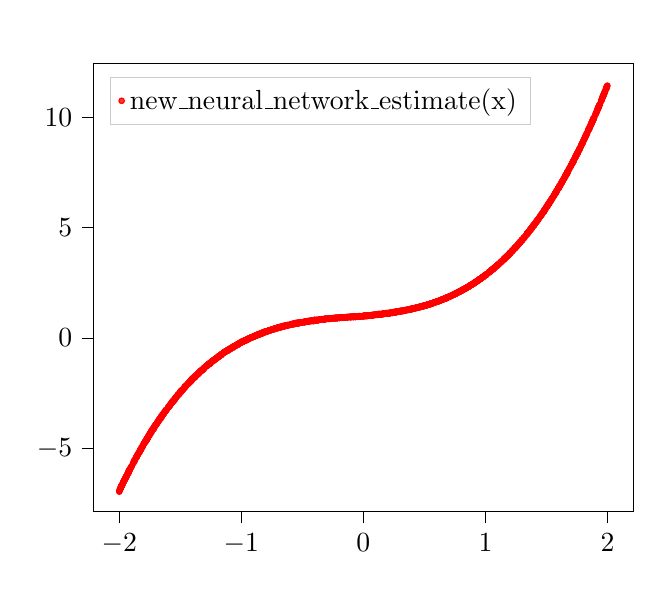
\begin{tikzpicture}
\begin{axis}[%
scatter/classes={%
a={mark=o,draw=black}},
legend style={fill opacity=0.8, draw opacity=1, text opacity=1, at={(0.03,0.97)}, anchor=north west, draw=white!80!black},
tick align=outside,
tick pos=left,
title={\quad},
x grid style={white!69.0196078431373!black},
xlabel={ },
xmin=-2.20852591900454, xmax=2.21306049239568,
xtick style={color=black},
y grid style={white!69.0196078431373!black},
ylabel={ },
ymin=-7.86405361849716, ymax=12.4391808546764,
ytick style={color=black}
]
\addplot[red, mark=*,only marks,mark size=1]%
table{
x                      y
-1.52762947004398 -2.63665679852607
1.74584146706459 8.30313418504723
-0.523478826928232 0.684981455327291
-1.73063347132838 -4.16754055824511
0.199724526357971 1.12413986692501
1.56583537106678 6.50212130573281
-0.463057519114948 0.747665654157118
1.27292037122199 4.25911843213007
-0.561300740541583 0.653996446870297
0.640763194967071 1.72674751050313
-1.73791342939199 -4.24096264611894
0.131982542924304 1.07163562445192
-1.83168405496555 -5.10376196338133
1.09632486787013 3.28860190499629
1.14869409291258 3.54804856022076
1.71062342784982 7.90152466385944
1.54063884052671 6.26233498072305
0.96036949117845 2.67188471681226
-0.36582225744249 0.829228691385662
1.03292095360504 2.98417928381415
1.57196496539069 6.54609386202508
0.316383914894403 1.23104885644691
-1.25339289598648 -1.13554910601212
-0.46394682067964 0.740299643711383
-0.998800252147865 -0.168876133428104
1.03613462412239 3.00699952570108
-1.64532444822729 -3.49293200198847
-1.97015264204063 -6.5769121469698
1.10611827964268 3.3325927944455
-1.40144531975216 -1.84518158676689
-1.71485775358785 -4.06883587132901
-1.55651601432609 -2.85466248166607
0.704149753887608 1.87137436411416
-1.35391349938216 -1.62114783985896
-0.19713428931697 0.91320639815536
0.890553629834266 2.41963800191651
-0.748635890255846 0.367757908994129
-0.0825495453396563 0.955542429515598
-1.52863234199303 -2.64905992413016
-1.06308264251695 -0.412431701954534
1.34829445246638 4.75822063973227
1.21677724541683 3.93402096649771
0.321064511493674 1.22796917544757
-0.79448963572049 0.286639405408638
1.29306522904297 4.38129536324555
0.991145476362639 2.81469205516578
0.408046183683614 1.33070158460102
1.50470887336654 5.9575393202239
0.241965856580386 1.14976159314043
-0.698625089638838 0.462631462074469
0.69277772759134 1.84475566662164
1.54249469168855 6.29223000018984
-1.37940963447366 -1.77397785165444
0.328552328283534 1.2358697609747
-1.76899063762277 -4.55181464197594
-0.1615118341785 0.917358084831994
0.979551973019646 2.76474222344531
-1.41400818915192 -1.93743608707598
0.920422122884637 2.5371272327229
-1.58813906344299 -3.08034023934407
0.567973302168688 1.574798756124
-1.7027550272339 -3.92661639975712
-1.66143052087379 -3.6310451778419
0.509387499079396 1.46884150329936
-0.649372469635067 0.531357119197573
1.27714939756953 4.29644865621161
1.99062920502101 11.3301714102496
-1.77767653093197 -4.60832173114591
0.95231808494159 2.65334945903267
-0.729339734657573 0.394415405360015
-0.69929992108586 0.469586842821553
1.62359205741297 7.03622721245334
-1.26350376928392 -1.15873251814128
-1.80495773362803 -4.87445067342779
1.4755075644755 5.72000202565798
-0.582140577898955 0.62882666918393
0.391595936124218 1.30969317341825
1.68359095958506 7.62901889841519
1.55014341230999 6.35669199872224
-0.461713591692503 0.760474080303689
0.837995109576847 2.25388599012062
0.0647111588263334 1.03231598849297
0.449501515148342 1.39080169134864
0.842450703096236 2.25731626328023
-0.662607691037783 0.514319433635468
-1.73347656811602 -4.21427270283707
1.97125407913951 11.0374500899417
1.06434018406928 3.1398766859045
1.24774144636567 4.10652488237163
0.301552235654667 1.22610695051265
-1.419054264094 -1.96851225748391
0.770735380506118 2.05529699022521
0.673663615667701 1.79826450863936
-1.20717318186629 -0.921117900268635
-0.410538504386376 0.765068471502614
-0.997783575545104 -0.190561556633821
-1.9247004506919 -6.06488872678494
1.67307707998314 7.51858011026587
1.13094409339522 3.46594756951591
1.05978614977254 3.1119281304365
0.368497683846726 1.27437039746974
1.19041117219778 3.77115160864485
1.53532876144759 6.21911480195912
0.977879415140715 2.75127965038619
-0.661130676558663 0.515515881624548
0.372560417149814 1.28014251982014
-1.41713935044321 -1.96759316741115
-0.721990537872462 0.427308795775999
-0.593304843043549 0.610478409782568
1.39782862521232 5.11259491405215
1.31945403787629 4.55774479220443
1.29797173081997 4.42915493648867
0.500221801881652 1.46197989702367
-1.22858048710803 -1.00927000019683
1.84901594258915 9.47648534922581
1.5150131259747 6.05407785409292
-1.22889583462019 -1.02559434722004
-1.4115062222231 -1.9348610640109
-1.33406864789987 -1.49095685339282
0.212784793779644 1.13119633500023
-1.35572868353146 -1.63622217917435
1.34923257581794 4.77328323295919
-0.117934710702453 0.944959877079549
1.74259492028609 8.25448605318237
1.79584748839092 8.8397486108736
-1.56683538172848 -2.9161474951396
-0.100670899179379 0.954539281248498
1.3130637409383 4.52476010808466
0.413802060319139 1.33744361353339
1.03952918317515 3.01003625023142
0.355758361430128 1.26871554742047
1.06587471434403 3.13952285378779
1.47827077764151 5.73417393797497
-1.423248862284 -2.00477990059306
-1.64138318843414 -3.44920568469485
0.858985773610331 2.31055719751639
0.30940079900652 1.21678960560482
-1.59532819132151 -3.11544889268605
0.674828392358402 1.79411719788582
-1.99791465316728 -6.92318765043389
-0.983915817371269 -0.150434192007041
1.05210422602657 3.08040038211607
-0.460520520996104 0.753445163781151
0.793577616390077 2.11102106409086
-0.916701943346689 0.0293686277642946
1.80568436851851 8.9740041455143
-0.41905914986584 0.775491286151664
1.4905136786334 5.85347534864318
0.659003889297849 1.76823560366373
1.33264972737708 4.64719307545267
0.367019067455185 1.27683076268824
0.284838881991474 1.19735122698525
-1.56586227893797 -2.91574117100978
0.865300493711527 2.33095887814049
-0.939391307968867 -0.027203254178731
-1.88319560164792 -5.6496600168737
-0.525375767528593 0.684583616019016
0.496152544580833 1.45177679093498
0.386055497083448 1.29164860153159
0.351299629919691 1.26288874499817
-1.65598010248621 -3.56432636874693
0.751560061269861 1.99687186057058
0.284661315211381 1.19235145843037
-1.09215628143104 -0.491573300112702
-1.10348826232006 -0.524640770030218
-1.00871955963086 -0.225586793602744
-1.54583226518551 -2.74904177692399
-1.55838780436906 -2.85682837025492
-1.03843932105837 -0.325694840270278
-0.946724153501291 -0.06049006215608
-0.654071049279125 0.525404355982477
-1.90500466748741 -5.86320237196585
-1.27255094354131 -1.20661238758745
-1.98026347546296 -6.67989024206411
1.63566363171233 7.14486566814899
0.0339713196359335 1.0093287980423
-0.50459247118296 0.703641359276434
1.81559893738786 9.07136373457222
-1.63792963751805 -3.43811065019935
1.81879951740473 9.11907419867196
1.78184093727109 8.68248370406747
-1.7721536426822 -4.55105725684285
-1.18740832757247 -0.855914984597267
1.38038656570182 4.99110878004799
-1.38783512640697 -1.78378026045502
0.222412885401944 1.12854784914632
0.756559645781282 2.00559445533501
-1.7219989420926 -4.1241360273851
-0.471086587199301 0.734105533462656
-0.227738431702199 0.89333543925946
-1.92935794945476 -6.12418892694745
1.1844290411186 3.73565569764499
-1.71501087455885 -4.0376542850963
-0.385903061117554 0.806071659467239
-0.890520314626398 0.0740593743595064
1.67287119794209 7.51115796744165
0.83918431164092 2.25650874404071
1.90289877922406 10.132856650788
1.03833740641711 3.01299290037405
0.789709020700827 2.10355162038978
0.683611022039177 1.82285368297838
-0.179507048827252 0.925081437742517
-0.000584604517955611 0.984340468812395
-0.520405730169149 0.693339417279343
1.92715956982417 10.4668434718492
0.400860795137212 1.32987293072187
1.19890765610203 3.81451374961079
-1.54460728333877 -2.74787026367663
-1.06248141493513 -0.406999040383797
-1.28672179531481 -1.26478539543189
1.25307005082172 4.1424154599753
1.42377930122459 5.31239619932744
1.70117716962273 7.82129096593986
0.179317666451924 1.12103935376769
-0.684304672411856 0.492541754858381
-0.868768205503995 0.139903632995063
-1.51891316821996 -2.57567499366925
1.36361253017276 4.86933885074933
0.0562416104519134 1.02593905383052
0.0758099949952324 1.03392765224946
-1.58113161808202 -3.01793810810587
-0.538980074292445 0.677534726364365
0.99270343344348 2.8231022276446
-0.409786318725182 0.789398428413281
-0.281142307585388 0.868639961816714
-1.69745666265164 -3.92386559000922
-0.370783589091509 0.804295606864759
-0.230187126417397 0.901809719586254
0.454070535352471 1.39744018922443
-1.49888350765559 -2.45181224972991
0.494126089847875 1.44129943661414
0.609683100231467 1.65241912894958
-0.416834592236302 0.790211066977293
-1.32562012581223 -1.46790146868228
-0.535019952703819 0.663209586913815
1.46284070470964 5.61791567029054
1.79853558911958 8.87579227219735
0.543964275193791 1.54269241151363
-1.12101167563638 -0.587903117238959
0.634585312093048 1.71296042187226
-1.42338564384549 -1.99995903396004
1.34323872565678 4.74249413175406
0.740479740191689 1.96380089060307
0.530420671662911 1.51309076141407
-0.652511983931383 0.521107180103227
-1.48154716489781 -2.34954351397374
-1.51975770883372 -2.59116390660472
-0.357623802961932 0.83381141128213
-0.873939423227781 0.125932421557286
0.819777580708701 2.1998943411007
-0.771908094224033 0.330724932627523
-1.25533466724185 -1.14123378490591
1.38048627129223 4.99804329532372
-1.41426900723107 -1.92000749326875
-0.931515071393668 -0.0230607378401753
-1.83612664651561 -5.19848319937411
1.91787399816632 10.3457425819134
0.822087947034545 2.20295568925398
1.58408998110077 6.67853165613535
-1.47666690758891 -2.32386558025554
1.59307040077941 6.74324021433242
1.82604877768948 9.19739450525777
-0.0643848869724568 0.961139915466772
-0.170247791580812 0.930901724014497
0.576780822247429 1.59740172217391
1.23866843250204 4.06837261252609
-1.59773061856609 -3.13496249784628
0.779140264391865 2.07272054088885
0.122981305271473 1.07007161647795
1.16018101227257 3.62053567845117
1.41737534405674 5.2489009736737
-0.125273475886996 0.945827754840978
-0.0752832772171206 0.969968969047981
1.60062278839547 6.80197787067499
0.672159440578955 1.78812444699988
1.74816251900159 8.29682205654595
1.52974515968788 6.17933789924982
0.818853077332124 2.19652244374451
1.17010851194556 3.67232407707197
0.669500173210326 1.77942747846152
-1.3832662134864 -1.7597563579927
-1.5056123093124 -2.4761572617853
0.676128404865428 1.80489610197411
0.354286326377876 1.26228019772993
0.110812810663127 1.05287390989139
1.85823905265138 9.59712772884433
-0.296690209866944 0.872379305015782
-1.87852985180451 -5.58878670482915
-0.561567284182094 0.647239410899878
-1.34797827041401 -1.58171359060356
-1.75450255430753 -4.40024872280045
-1.65803450911699 -3.59862420326409
0.899307716725425 2.45310985507215
-1.46062397932672 -2.20590832094584
-1.35397611455221 -1.61410551820944
-1.55462920986326 -2.83631479759145
-0.325694520641469 0.844135792066377
0.160385508824723 1.09385491556522
-0.0461815331773878 0.972733177334569
-1.99131143951082 -6.82898935026358
-0.974657684229868 -0.126816225683027
-1.1961708928454 -0.871963915385551
-1.08638984261912 -0.46817607178617
1.87310279781129 9.77910038124017
1.91185810187506 10.2346177433489
-1.14125893032288 -0.651143612967894
0.528322311654728 1.50440518127949
1.72555442756985 8.07019342203641
1.49516179008768 5.88943360017781
1.76908731382206 8.54319474425647
-0.98536492396836 -0.15700092510946
0.822905514907454 2.20331143461938
-1.9175384908525 -5.98579056838029
-0.634376195176915 0.557193522846342
0.803957485520665 2.1390454266119
1.8795561718596 9.83452954613513
0.247638382220518 1.15926441782563
-1.71883857673055 -4.08546459916181
0.391903377619543 1.31389415981742
1.03697635833877 2.99252053203022
0.46546627101158 1.40460445522065
-0.872255355483843 0.12452919017408
1.59963770381937 6.79624745217679
1.0905089794862 3.25222839325567
1.48364736751732 5.77669503094874
0.552152149540717 1.54712047919933
1.16305110024444 3.62821178894314
-0.764162395575607 0.353582332679796
-1.7996558729966 -4.79060711409738
0.257994234634654 1.159234494009
0.975819193435273 2.74312471916832
-0.374068096434548 0.811941703820846
0.732361402874449 1.94289288266549
0.841017152420385 2.25753945477373
-0.317325089675505 0.852558721839276
-1.14729985819558 -0.679405812472515
-0.84115142375628 0.201590836168429
-0.195889906726145 0.914464415551292
1.2198790586966 3.94647009708091
0.153095278361347 1.075407139745
-0.721646086143089 0.418113274550875
-0.276444233603721 0.874891330907061
0.997336602107659 2.83914267877571
-0.619971894263125 0.570644133479019
-0.987367251982856 -0.162659397984739
-0.854665346688174 0.163321947347233
0.191712135688579 1.11008010260121
-0.574488728271056 0.632500385245556
0.00863800784050106 1.00372572314337
0.307398788784521 1.21625487746565
0.342728984756977 1.25802380214618
-1.68981021594347 -3.85635974658295
0.784208901049624 2.08772138448435
-0.208369439125148 0.913988845682418
0.526648200820822 1.49948454846173
1.24202756976366 4.07702962445207
-0.727519971518694 0.416619346588576
-0.222858774302506 0.899970690899377
1.42817273628317 5.34391409346648
1.38769399086101 5.04512706115714
-0.41333614984213 0.781506781386756
1.30000904085596 4.43810676743973
-0.0370187504556303 0.973900549312141
-0.381829049097851 0.8006227077616
1.29945975418766 4.43145515107368
1.69798018089684 7.76034437975662
-0.978298825314186 -0.12745101956886
-1.66927279889651 -3.67091481981135
0.606203457135684 1.65452552319128
0.211301964437266 1.12170481513714
-1.00052625391862 -0.198810328948178
1.19345373102677 3.78511354553779
1.57544991206892 6.57360192278671
-0.77491023651087 0.332263920464899
0.159718334398355 1.08833688203287
1.45665398404387 5.56727126547789
-0.499484712478448 0.701589152523506
-1.16220758413343 -0.752574336865251
-1.02136658157845 -0.258844629313983
-1.06674862945718 -0.392686634605278
-0.744757010347744 0.379338217369195
0.623435205569478 1.68225418863393
-0.0599727657251976 0.964843293712371
-1.6688985298492 -3.67191162329495
0.00795195473762167 1.00095435444599
-1.58371970380259 -3.04223877021898
-0.814488977715953 0.25400468163354
1.62784684311749 7.06018606462141
1.10659216693293 3.33647695876888
0.746100055298261 1.97888290220787
0.004435567456055 0.993685051475752
0.273048244481866 1.17750929462584
-0.674494714349047 0.491965498520511
-0.630136777628819 0.559016438722326
0.404649191564105 1.32802772062289
0.867192246641215 2.34518405432025
-1.53462890319051 -2.69450269874947
-1.65797847179726 -3.61466929551865
0.936206661941811 2.59443165886383
-1.78249170379428 -4.64964642499287
-0.989577984804854 -0.170243909850942
1.74689924571509 8.30477247920927
1.36878773996584 4.91833067708624
1.85181571111122 9.50239345194755
-1.74027129194973 -4.26582547182024
1.32195369830832 4.57287695579038
0.779295097985163 2.08547213848138
0.527134401728108 1.49717159191067
-0.483385457457882 0.721013992566675
-1.98054469090637 -6.67787951840296
1.19919838050934 3.83794979312015
0.247147941406696 1.15388799111552
0.0973894309066896 1.05036888897258
-1.41470298624829 -1.91867719201216
1.22947358771133 4.00233387501312
-1.94803996825382 -6.34115402871578
-1.37522052503804 -1.70312718709698
-1.69508729758743 -3.90422830135512
-1.26400612715092 -1.17882495195713
0.177514997367698 1.10070307970624
-0.669640851903173 0.506276290801674
0.67112924906392 1.79045933660594
1.50698404505808 5.98164127150539
0.0503843989658583 1.00362100010182
-0.479836536391115 0.717791570047364
1.90580750567755 10.180201922895
-1.95045988746964 -6.37125640924513
-1.23772859446057 -1.04768655971777
-1.2491992534694 -1.09917023861416
1.43020405218296 5.35155575358987
-1.7958406700768 -4.77516846470591
0.6793613225212 1.8200682595746
-1.46040150163991 -2.20800476249903
1.73771962842721 8.21560467911202
-0.84730566648012 0.181473749770297
-1.00894166771783 -0.226811317886355
-1.00859420626261 -0.222584462396821
0.958638844017508 2.67815991960788
1.95044573476592 10.766490129105
0.0346133021748543 1.00994873094911
-1.05062638029796 -0.363128077667757
-0.0934869135279128 0.949219762303069
0.210153076911402 1.12020283425862
1.06304622638943 3.11894277339172
-1.4913720899944 -2.39900388339497
1.60616168357588 6.85479758268493
0.330881009604624 1.23690985922366
-1.41434542654993 -1.96193001839419
0.54827261775172 1.53292166739015
-1.05020516352889 -0.355253516364615
1.99084203167489 11.2963039571817
0.284498672856374 1.18803669814785
1.20635571406931 3.86687589245562
1.92884887664005 10.4605744830663
-0.787836212255184 0.299734103526356
-0.0665370859942191 0.958109369188055
0.266365751071064 1.17365638382964
0.284821733614269 1.19864673269428
1.79658899705357 8.84717765083633
1.36800009261001 4.90984160895382
1.71913709666286 7.99583556443286
-1.64691824710695 -3.47709331465477
-0.634577139004624 0.55915870436024
0.907611460044221 2.48490211512442
-1.31752746635936 -1.43220825506977
-1.25799147179641 -1.15868706829474
0.164578863753904 1.09458335531589
1.5724728529926 6.56004765078573
-1.61334505165664 -3.25225593055653
-0.884101245130284 0.0929428769915395
1.0785857201919 3.20491586289296
-1.93700500597912 -6.19805198060372
1.57399805208916 6.56459550935528
-1.71744427363904 -4.0708018208458
-1.05808128539432 -0.384282057908827
0.335865050135636 1.24121539994481
1.67249976327608 7.53111403985285
1.60127860974401 6.80875163915128
-0.517147816897207 0.69333488423439
0.641324841192098 1.72460209308304
0.676786295025203 1.80733330661154
-1.82794401593092 -5.09710000332624
-0.283331862331161 0.87196176011591
-0.0639641528388717 0.966729126839163
-0.506504957395847 0.707835320922324
-0.916554913203721 0.0288747985266691
-1.74864875263597 -4.32050250007612
-1.22417132700887 -0.990462261382918
-0.480427977583389 0.737086525022445
0.522720217749657 1.49225304695111
1.79977796292236 8.87678850979209
0.821654982549636 2.2002667735956
0.705451304778161 1.87003509143419
1.91752469627165 10.3449889069322
0.874637643884115 2.38294790188029
1.51463407476122 6.03663515683795
0.151964456223034 1.08602328208579
1.04920814119334 3.068717656264
-1.40228679868784 -1.8703882159323
-1.77433062051123 -4.56898824875179
-0.0807199561361247 0.950590991918523
-0.554066225390007 0.676013409967546
0.206793034906914 1.12162283249017
1.75495320295264 8.37161770096163
-0.58976643547149 0.6122332590153
-0.570265564796054 0.632088878798852
-1.95652629667675 -6.43236712937771
-1.4809655079249 -2.34962300810275
1.24656860874358 4.09436510331362
1.04805738906209 3.06644566689696
0.245998012934822 1.14616974570374
0.712250733621294 1.8985145336873
-0.178999679781882 0.937689573199967
-0.476724521976923 0.732967579431614
1.57873780306787 6.60316766960317
0.492905548214301 1.44673427787968
1.96692074715421 10.9935413794022
-0.866109375642834 0.137806550330372
-0.902579722541617 0.0533495254779157
-0.4836989537125 0.721480405653948
-1.13860622829876 -0.65812494496624
-1.68674389282483 -3.8269478035141
-0.696380684896323 0.462339397493708
-0.474718614621026 0.746846022399951
-0.55910870278528 0.649211265691872
1.82989710207585 9.26165707381093
-0.747639397853016 0.384910459455232
-1.21735597090758 -0.980617456389869
0.370162748415718 1.29014014231753
1.52374645718827 6.10901973485953
-0.973366382246718 -0.131009116090045
1.16171016526292 3.61697168798142
-0.862987828535092 0.161078907132451
0.621063996734559 1.67901339083638
1.65446335556188 7.34017160890469
1.77094426801913 8.54839534495773
-1.94388635474945 -6.28311770959015
0.761200781796524 2.0338355887882
0.0561172373005312 1.0213583364538
-1.06957567386867 -0.411001296441611
-0.0905481850787533 0.959183499127584
0.927040219844024 2.55424325573772
1.8673231985492 9.70422640604761
0.192108321913312 1.10176166062749
0.513399284106047 1.48857011176581
-1.94821049397743 -6.31319466428297
-1.1214590808955 -0.592631271826917
1.87606393659345 9.80087088545134
1.84450991390793 9.4353368625487
-0.049463327121563 0.977076978786467
-1.18160442071139 -0.836295878091666
0.304089057238058 1.20940477365912
-1.59280051013905 -3.09419187436563
-0.949890380048008 -0.0644734829889833
-1.55324124736082 -2.83858147926448
0.447202411694953 1.38807365079743
-1.34200036036863 -1.5262171878444
0.973498301084059 2.75044470769863
0.177052608250697 1.10709754591426
0.0405965700044342 1.01925157212804
-0.752339810673941 0.37289273972447
0.168360846647789 1.0924382059155
-0.147385650667953 0.935925901041053
-0.0765706138124309 0.966310494501428
-0.834073223482545 0.189431722979178
1.77400258345304 8.58815547506922
-1.10923369352111 -0.537029360030512
1.47731730787747 5.73058332341255
-1.97426591551265 -6.65678088227076
-0.46465919100746 0.743422947401185
0.255453290103878 1.18141978600141
0.401946609783347 1.33135091302226
0.7064603645273 1.87840239998449
0.195040572032665 1.11690200145903
0.492725116630803 1.45754533122342
-0.703358333592255 0.454883515873727
-1.77071940640349 -4.54100131963547
0.0263778409957616 1.0146304100638
1.5817323511687 6.64653301342941
0.188973280062564 1.12135526154422
1.00105500765951 2.85977988013338
0.665601496451699 1.78226977757198
-1.0758927035242 -0.439445577528765
-0.628467864929659 0.552521016834506
-0.462845639931512 0.743649977634857
0.875025914541497 2.37374222271564
-1.41383683667054 -1.94667718809135
-1.6697111938579 -3.68486173375494
1.09603549914051 3.28567858678585
1.62489834081238 7.03690114243045
0.416808458329184 1.33498770793675
-1.91346899374008 -5.96256237772706
0.48890415351061 1.44286865771006
-1.82702980036481 -5.05551592861472
-0.271371741436216 0.870328942223097
0.0838712538685789 1.04189708615533
1.24655440116632 4.10024175055629
-1.46183141783321 -2.22374166989591
1.28908473130799 4.36630170768102
-1.10855990085608 -0.562063462639219
0.933803589297539 2.58521487037548
0.744090662949441 1.9707947494304
-1.18542851197 -0.840491037489215
1.09662847195115 3.28482021885626
-0.891904969622721 0.0831156169344429
-0.753767622372932 0.369836018957886
-0.419699453159715 0.788081674304745
1.92783611898138 10.4584854988399
1.18434629483526 3.74481770501953
-0.850048612766949 0.176560415789933
0.308458399857949 1.21462782639147
-0.104193997970978 0.946005898372418
-0.799972736430903 0.285927701009198
0.452767708690214 1.39766719368028
0.597412080517727 1.64373993259383
0.593059513923374 1.62427200463893
-1.40250057451328 -1.8789264057244
0.798607175412876 2.13331105315066
1.93257294274525 10.5355389630815
1.99854849151513 11.4244399794226
-0.641668732087585 0.56475366966752
1.30016400132094 4.43814008524292
-1.5326104928455 -2.67493541839968
1.37502262423487 4.94986951331791
0.693800378736968 1.8515716644279
1.84517395726995 9.43599452837678
1.92798071190122 10.4753358247517
-1.40772643694339 -1.88214066370521
-1.28601120370353 -1.26647654672643
-1.26627685651145 -1.18784224817778
1.80731301646996 8.98912832188046
0.90850383276711 2.4863705914669
0.0979589637191518 1.05077299541241
-1.49663558808682 -2.44076085587208
-0.912437419464073 0.0290584337091611
0.877357979495537 2.38865486323248
0.166820627653863 1.09218585818911
-1.77159986131449 -4.5633205102713
1.30437703030859 4.47265186631175
-1.3499326931183 -1.60225917189635
-0.596182841232093 0.608163392297305
-1.87620318613111 -5.58351911620609
1.39855464279318 5.11359242740474
1.75283927641585 8.36942259144701
1.73162706612773 8.13826599634615
-0.766719221853512 0.340864384170174
-1.92279238876334 -6.02321863912057
-0.69318058382554 0.479668680603467
0.00831948249165038 0.999751590490404
1.48305548603697 5.76142487230455
0.153118246334721 1.08972946434602
0.58443191408571 1.61378691004878
0.236693925468985 1.14339170496782
0.646310871944384 1.74030084845718
-0.398390991704618 0.808366816187522
1.62011872039472 6.98953178832817
0.163170880205424 1.09101052685306
-1.05611175254839 -0.360223134163143
-0.450061164749038 0.760914089150395
1.08455697511961 3.23431779839021
1.07031030216604 3.15892859213176
-1.13369677432869 -0.640947173373567
0.954869425914125 2.6738604387378
0.190796234602346 1.09960866645781
0.34599075164786 1.25596865017729
-0.0417235161195215 0.971710379783804
1.6996522021834 7.79550916409845
-1.98068498864511 -6.68203605801189
-1.9115004631109 -5.93364414254743
1.53382768152136 6.22353879720709
1.31412729272728 4.51961993490372
-0.685326460329759 0.47418665950724
1.97256061584938 11.0547994580786
0.520690061019052 1.49111868744377
0.431498523136836 1.35789622587648
-1.54362657653036 -2.75460998020516
1.30076943936791 4.43975314877167
0.110705357748875 1.0486479677216
0.0688186092254197 1.02119784489148
1.67413450951731 7.53341721455009
-0.985207968505172 -0.160684540430415
-0.806089795979227 0.284444176437579
-1.85237667046108 -5.33233210062879
-0.920371820742431 0.0164668433527722
1.38141443382448 4.98863015282167
1.4044209338851 5.16669611818724
-0.542691600248609 0.675735850532089
1.53677101777 6.23346451860097
-1.85850522725861 -5.37882491327555
-0.444161392146742 0.763771158560042
-0.688501376551688 0.478927137327461
-0.593839572757993 0.606594772417755
-0.47441079581978 0.741345605082063
1.8831706950332 9.91285698162258
1.09169014263716 3.2517433215441
1.25389927608542 4.15534414662229
-1.59454200048405 -3.10600040525396
-0.442711305472325 0.762550665143076
1.95806353082891 10.8724704838653
-1.78460742639196 -4.68605248225971
0.40343560525519 1.3213194545941
0.652220564362389 1.7449551608856
-0.380836178645997 0.813053290144024
0.301719509164299 1.20512017543195
-1.21097150035761 -0.945192574788016
-0.029223722261007 0.986101783902391
-0.0358890414286468 0.967455226587691
-1.73775276817218 -4.2353480015459
-0.974754376510504 -0.1267811188567
1.44203622854204 5.45062670730321
-1.59890642565992 -3.14658288961961
0.795623049507605 2.12756096210532
-0.150922502332556 0.928688080958424
-1.53940041912788 -2.71723181405971
0.0487454727564445 1.01873554029746
1.96324448991474 10.9345743710465
1.66781793345191 7.45481886645438
1.73884391761524 8.21231629267577
-1.92817622064621 -6.11153730590321
-0.45376515808234 0.739633548853883
1.56230883155345 6.45409691855904
0.54828212047107 1.54415654792256
0.442437873944731 1.37678215206925
0.192524261196695 1.11685238085851
-1.18547716382506 -0.833172875923745
0.131479945441129 1.07644065677529
-1.09917176544636 -0.529014837658806
-0.470282670431948 0.730487027283281
-0.398534332506407 0.809759655887622
-0.425917514759681 0.774729820255762
-1.20315602945709 -0.901621628900615
-0.658854777674013 0.520887961468839
1.90279869634687 10.1535144403424
0.692627430585937 1.85850380394309
1.75702419283417 8.40248244830576
-0.218196717797614 0.908040475854448
-1.78916450307182 -4.7072198549223
0.129070596408469 1.07891023355875
0.605038800031316 1.65138168952477
-0.296316256804238 0.867483154147729
0.0164951209081132 0.988124447555131
1.21346412797034 3.90729131164088
0.574011131001371 1.59115392326239
0.462290671416839 1.40614477192918
0.40410819275721 1.32633180954348
-0.481595493587628 0.733282230587212
-1.31782552436269 -1.43093933687504
-1.5194837321693 -2.58315848179824
-1.62116265544403 -3.30344496903047
1.26310081801528 4.20151526945381
0.127202279000513 1.07081464024437
-1.68520250790848 -3.77793523091417
-0.603284843250533 0.581234017543621
-1.71673296848097 -4.07683475528603
-0.532651132542052 0.672261847207747
0.261358540370296 1.18512451859773
0.558581812877678 1.55736841573768
0.666199452291657 1.77515665700216
-1.00171427776995 -0.204103549526015
0.216887403452102 1.12488879547923
-1.66491700448442 -3.63645953599789
1.62371233364995 7.03647864252876
1.89298814563213 10.0075273939971
1.99696540172668 11.3985956317353
1.49857458851087 5.91810351458466
0.0259271242716275 0.99490040667827
1.25066053839307 4.12725819342969
0.741554342666891 1.97024401050884
-0.211134376905973 0.904265588112284
-0.21293296225532 0.902208372935693
1.17443099534439 3.68928772174936
-1.81670082980822 -4.96647251739284
0.236732509242013 1.13315323922089
0.643870709298875 1.73772272122517
-1.72227657824281 -4.13521216446846
1.63583921447564 7.14238562238487
-1.68186374417258 -3.78531224191223
-1.48826071885157 -2.37873968411393
-1.49310781433945 -2.39855010937928
-1.10696078276606 -0.543277142424544
1.12452649312155 3.42889377843165
0.783650456241737 2.09083865222502
-0.161911748499459 0.931137194158423
0.628007684776644 1.68442530419979
-0.243924773625153 0.893116388521999
0.834772814765674 2.2351337827488
-0.223841541824117 0.900516913726931
1.07132477350497 3.16306477307216
-1.18266111651542 -0.832822823434673
-0.428500086152374 0.778049775291733
0.90169194696583 2.46648254129569
1.09745444799678 3.28796605696869
0.523909850278403 1.50151748649013
1.73717403201051 8.19682065367904
-1.22113069512167 -0.995120760996621
-1.20955849396782 -0.953255169415617
-0.399486529556002 0.808781879310853
1.45060068843825 5.53087848795961
0.495836028886981 1.44879256164344
-1.54563926520025 -2.76119064927738
0.664636176471893 1.78163979951814
-0.84536772623423 0.195978403180779
1.84784612583578 9.444972752919
-0.102234273221019 0.960155648523784
-0.92791030503047 -0.00201279096713414
-1.58862031670824 -3.09677838620582
-1.40597534148641 -1.90921472245161
-0.0567426886504618 0.967309510794382
1.95112557211344 10.7836771757371
-1.16202891862751 -0.743642158251616
1.21626034128942 3.92421811806867
-0.80452779989253 0.26609097967275
1.92498870321335 10.4303878655003
-1.92515688031637 -6.10821307405095
-0.852504867179035 0.170600669614789
1.55705189462523 6.42445316743795
-1.51788427122346 -2.55981081658546
1.3689591098897 4.90303972175912
1.75972680655051 8.43497694100864
-1.65957374583011 -3.62665673598408
0.270920890606869 1.16949282304471
-1.16885208042951 -0.763987666325113
-1.38447964389345 -1.78579113660629
0.177339566960526 1.10697129299923
0.543295442544644 1.53305438086109
1.81238014720433 9.03883120895235
1.71910415517618 7.98951188473036
-1.38574884153756 -1.80453591712449
-0.866168705486111 0.13155224998541
0.56542842101778 1.57148386121625
-0.999358479402314 -0.195291929222586
0.517148701909557 1.48294034813878
0.385827101406312 1.29470435488792
1.5126698410979 6.00707691823652
-0.847485819932245 0.181307650065231
1.37674588490367 4.96367311113197
-0.836170270341625 0.192930597010434
0.772951559632365 2.04951697969711
1.59583203319957 6.773635455285
-1.82180810974138 -5.05045903144996
-1.69300170047109 -3.85896485817725
1.44794960970744 5.4999476493892
-1.66109627169685 -3.59464056731823
-1.7573382699851 -4.43118186833144
-1.10719019711833 -0.532950161422905
-1.51256371702266 -2.55738152032505
-1.2165312811155 -0.966154532794749
0.879251925733673 2.38729259303622
-1.87054596694108 -5.51283413585285
-0.441182691897304 0.771939195941864
-0.19493987501971 0.911954170378767
-1.37728571964468 -1.72844840209457
-1.82483177421839 -5.06024739494962
-0.702010881428292 0.451843329310979
0.326122906767451 1.23172693663433
1.16851737260205 3.66289673262974
-0.214871572242574 0.902305420744069
1.31468918333912 4.5327764118568
0.62424958546635 1.68687541631648
-0.41248770407115 0.78026988517054
0.462518280013717 1.40117426976985
-0.876558973447731 0.121068561770403
-0.445309663339691 0.765122542337629
0.286003384268398 1.19420332378833
-1.38403511544209 -1.77359364826383
1.88068779520718 9.85376193718621
-1.6185680719818 -3.27523195342785
0.152180559735233 1.07754121780664
-0.109158171926152 0.94797019633471
0.24651978919582 1.14965891306799
0.628965416458113 1.69882274744483
1.91935588472357 10.3540013605604
-0.0373830886566422 0.976154099548856
-1.68054947050608 -3.76688627554973
-1.87451027850194 -5.53804599169035
-0.555079240761019 0.66428892526408
1.43463336473141 5.38729732564786
0.296471880579543 1.21214083308364
0.596403994269193 1.63471382573155
-1.9599885782736 -6.46862056778319
-1.18377169591759 -0.835764211058809
-1.06598170603066 -0.406347917054451
-0.0744541532140537 0.970544054476839
-1.76337010414204 -4.47980815903837
-1.09667441590765 -0.497958138448634
1.62826999259492 7.09346422247264
-1.66496683308716 -3.65859501527713
1.1752654100337 3.6867880267327
-0.711313673950508 0.441159206437018
0.949181662762235 2.64913485004861
0.23509675462388 1.14631030410878
-0.132282055480576 0.951380021157754
1.15162918388688 3.56590005483656
-0.825309704656912 0.235428161007987
0.0416208378466676 1.01916426816218
1.28237397513989 4.32803419372785
1.67804663468333 7.57560936511758
1.12847037380373 3.44583730827938
-0.666677668801422 0.500535466902455
0.0771935567965247 1.0251579835824
0.382430291118693 1.30125913420781
-1.75396408351992 -4.38684640189132
-1.27713484050294 -1.23728764579277
1.26371408079828 4.20747471043581
0.631521703007308 1.71097872801138
-1.9927489392525 -6.84210703404694
0.429833334690461 1.36756426971277
0.885000450618656 2.40899164257351
-0.928739515085039 -0.00112897243548949
-1.79090100863839 -4.70858495483779
-0.190402521964136 0.920291720165465
-1.02277075142579 -0.254672518218796
-1.98986414127296 -6.81967763997728
-1.56202189656636 -2.8700002969686
-0.823305383673487 0.240385903454283
-0.16535725880631 0.924942878158168
1.60375707727229 6.83113643466909
0.473228880387381 1.41554736679962
0.265718505149918 1.17273273686391
-0.0597395478923923 0.971368513214256
0.300775466668908 1.20781495684076
-1.05886021200778 -0.380369566542633
1.57753799391147 6.60566982934968
1.2678036676601 4.24054628185889
0.408969622909501 1.33434109200796
-0.802400565314632 0.289453107342089
0.797390436275073 2.11921434311487
0.269292520108907 1.17748066233802
1.09863981296441 3.30238844951017
1.66270555828155 7.39872202244838
-0.0678474745177926 0.961163352850507
1.15694791286823 3.59120166028488
-0.811165066606464 0.267983807143246
-0.948634762579282 -0.0490322431644212
0.98120715897871 2.7593947116178
-0.228724559837756 0.900312851955522
-1.37228948746877 -1.72229450435978
1.34818409339734 4.7540661109
-0.63180800074183 0.559632310925091
0.969694764923288 2.72146353859967
-0.15563669746887 0.925302312133414
0.732961867207918 1.94489665160677
0.985039768614193 2.77722119348587
0.320869401360116 1.22146660615769
1.73657869247921 8.1709769068018
-1.48569607335105 -2.35751632668528
-1.67052307021378 -3.67684260041769
1.80986213936798 9.00751847410175
0.269901033496012 1.17497245115711
1.86964035709248 9.72053894079343
-0.618116427779094 0.57948319057898
-0.559013229623111 0.640029635332599
1.86053966331359 9.62113266205902
1.83639477816247 9.32089258884026
-0.144643275194269 0.934702694488004
-0.661368634771165 0.518005380333269
-1.49996211674519 -2.47060303978315
1.61565620264765 6.9556738208655
-0.525992789448132 0.690153670706809
0.616639082134211 1.67233716321322
1.11048851688358 3.34846455523854
0.490327890360109 1.44696062751948
-1.70630821016035 -3.97942357433033
-1.08432082336125 -0.447866032025121
-0.470247615489478 0.737040127491929
-1.12330616920672 -0.592688203625215
-1.01151194857804 -0.22531529845062
0.93537143033542 2.58899557709597
-0.780955892956971 0.32494943131485
-1.64128116553575 -3.45549750121784
1.19263378023814 3.78334139440739
1.10397943127227 3.32477236366575
0.564707687955063 1.57096864135258
-1.07973399874306 -0.462843967286802
1.20149098397145 3.84041420340939
0.695933299560299 1.84328315610021
0.495176883716653 1.45111124871371
-1.67550375125215 -3.72282087079692
-0.529803028699704 0.67391141147433
-0.445856021780258 0.746872603821456
0.433812532010605 1.36821956949014
1.54202085374851 6.27014082733516
-1.32375381765984 -1.47198532477877
-1.62134922807424 -3.32157292176848
1.51933493963951 6.08477696358128
0.471822244683532 1.42329463587884
-1.7933624880284 -4.7584821763407
0.596742359496119 1.63294109206395
0.552130519421354 1.55492174251572
1.47710227591609 5.73121027778143
0.00302994761583175 0.998517527547431
-0.236203654112023 0.890720008570176
0.970165770754015 2.72487587611247
-1.34277493490018 -1.560845574621
0.206076871985257 1.1257152390431
1.46412316541014 5.63221243541157
-1.80601682524143 -4.87953733752454
-1.391266729644 -1.80715428918603
1.88631551186505 9.94610960451085
-1.10746678059245 -0.531319186183653
1.05027379222569 3.07342814811358
-0.542183740128499 0.661768181124191
0.0271656137687568 1.00594390041955
0.298087731551128 1.20094009138946
0.434215781068596 1.37296325698884
0.853518173197716 2.29721032854808
-1.02478655719921 -0.278179128954753
0.930280869478582 2.56653063252946
1.282077171204 4.33841398892212
-0.867967962223037 0.137217640904829
-1.77505278071821 -4.57906190273618
-0.485529113216811 0.70779431482014
-0.935709399072525 -0.0297072239274747
-1.7124804972844 -4.03787929313712
1.7597432806956 8.43146031674183
0.756160878053701 2.00445575272812
-0.00706127845737115 0.981964054736906
1.8189676207847 9.12539100938857
-1.43708373555605 -2.07284379552645
-0.391867214393602 0.81005629802083
-0.125622315968765 0.948908915942806
-0.227608808523419 0.901222918334211
-0.771183404944305 0.339516244786058
1.46047134279569 5.5976889022238
0.467766545173386 1.40672102796338
1.95848779282826 10.8896618409186
0.864335094856651 2.33375476079497
-1.63506328198021 -3.41060197363597
1.71568012752807 7.94562910214681
1.39272912489522 5.08961515331874
-1.22465164856736 -0.999370845561272
-1.02616643763754 -0.281109670883781
0.442734584377311 1.3636453659406
1.22412292980746 3.97718119164815
1.97421205804188 11.0926394512552
1.48145057673646 5.75859204672228
0.819496054168538 2.19628102305374
1.4980055219723 5.90529065694513
-1.18573895693203 -0.831044404668815
-1.99278274877207 -6.8494856711783
-1.91941536557922 -6.03689343835302
0.131241931655927 1.0600975339464
-0.580657766359237 0.621323641971421
-0.888088359400202 0.0879748598093739
-0.499052602078298 0.710622739621337
1.71820673011863 7.97388064367148
-0.316414951511492 0.850172933138876
0.393727886022705 1.30739732012249
1.00589706885763 2.87467650861009
0.57688395039735 1.58492314006907
-0.426697312104449 0.778529184768187
0.375189921780094 1.28553206713643
-0.813630157701015 0.272796922860551
1.2372573491537 4.04711291749065
-1.53832901940263 -2.71516049093013
1.35062857979094 4.78353830796967
-1.33694973116921 -1.5097033149936
0.564734755108878 1.58133376269604
-1.03761236511533 -0.304364625652098
-1.7347823407846 -4.19876453668963
0.945711070922103 2.63280043844309
-1.95258942984414 -6.39542582524028
0.0826143577681773 1.04656434275939
-0.511421420547976 0.700390007367014
-0.689362310384055 0.484189815360375
0.954490563853327 2.66189127695141
1.66434830933929 7.42551155767517
1.83138414083698 9.2535906483007
-1.02932672246069 -0.302454377177136
-1.04661156110905 -0.349194696608168
0.805645153296944 2.14727751708212
1.77401916557127 8.58561787796415
-1.40235998658197 -1.85626609020103
-1.0095984473455 -0.219611478121682
-0.270919141607282 0.871927628762499
1.2570941367174 4.15531025075
-1.86122822980676 -5.41679154352957
1.84661759143133 9.47138804968631
-0.90332609244693 0.0560399363281534
1.39563280875743 5.09338234894223
-1.98651168890195 -6.75881861620785
-1.9996278349795 -6.9117747602424
1.35079226518494 4.77394550653772
-1.79705482162434 -4.77476543435062
0.733839749036802 1.95167204064777
0.825728470288538 2.20865121947308
-1.999966065817 -6.9613984030445
-0.843299266844224 0.208944452179643
1.24300068592906 4.09229023697789
-0.568510673671339 0.628967296580392
1.51908286676269 6.08838913446026
-1.87867682212743 -5.56365333032191
0.51612906772595 1.48055749728735
-0.859068978962361 0.154159105057622
1.94861230872647 10.7340006651497
0.0534360058709065 1.02654421919225
1.15519390843326 3.59722956870279
-1.74527861230335 -4.29824285096523
1.66524052084331 7.43899384484359
-0.325981587735932 0.836218281066738
-0.752689738584645 0.372297506566086
0.128978317546487 1.07630978592339
-0.5621304215494 0.641110563792218
0.955494604929388 2.66243994646497
-0.555682648203415 0.657877220211347
-1.94548297516413 -6.30660150158887
-1.43026669699117 -2.03133524617525
0.356931141155441 1.26497851786683
-1.77861129362684 -4.64027561767086
0.986070692175463 2.79238643308185
-1.12135417504645 -0.583873973582881
-0.874192151028235 0.121619859150448
1.64662777642106 7.23880275344668
-1.36031739836864 -1.63023469181487
1.43962972373616 5.43679065708496
0.452585949580314 1.38020612816226
-1.76731956908791 -4.51087184778122
0.407565146203995 1.32590473134467
1.98898051125618 11.2966858096881
-0.598156498020338 0.603843415879494
-0.331884353093339 0.843716252343694
1.9650023216185 10.9636901570038
1.47465463159076 5.70579701648684
1.5204818278323 6.09842556468083
0.382297270832394 1.29907946604983
-0.308472069208821 0.86452974033168
0.464213345558603 1.40962225619966
-0.313121928977522 0.851139529144977
0.404197074317428 1.32297254888198
0.106771342877163 1.05328070645161
1.23841881398682 4.05574132595654
-0.282973759325347 0.86927530549534
-1.73525840893654 -4.24571728575114
1.20188368354561 3.84484408833895
-0.429258807295439 0.781389744582732
-0.748427956519946 0.38035750152032
0.0804517475120305 1.0282753335618
1.97951469313928 11.1614158365608
0.124479142005626 1.07152735282127
-0.68196947072659 0.478051156977546
0.223057422568356 1.12770066107423
0.469529140163063 1.42042477119935
1.81420517068728 9.06347397745196
1.09682487909601 3.29017544589656
0.914181350597536 2.51081156794732
-1.44096664107871 -2.09895744289672
0.659760682063931 1.77014541399254
1.04063674372985 3.0245021484701
-0.410649290239818 0.772472104365948
1.18214697910478 3.73390336265526
0.672531383775982 1.7818910668283
0.833061843126512 2.23739284468989
-0.617849314672589 0.576766640827125
-1.07259635030233 -0.439464162323758
0.391562842556896 1.29947440262709
-1.32972617708255 -1.48797880023631
1.70646260742689 7.86914077390867
-1.30706265571546 -1.35497932712865
0.187434893599617 1.11386759115505
-1.73820046861836 -4.24171387296479
-0.953602384085788 -0.0634957917389822
1.29875352212481 4.43489366176754
-0.103768824953191 0.943596096010008
1.78570975428274 8.72670519279494
-1.53634762343696 -2.68365510961318
-0.845841128729985 0.179914162737134
1.96130458726239 10.9217955746843
-1.38123143847418 -1.74150095436957
-1.82357045233629 -5.05015042661105
1.17694940504624 3.70540656238348
-0.810272952936271 0.261757370921051
-0.991398036985326 -0.172896205243066
-0.961061734282657 -0.115018311465007
-0.214642191506338 0.912795507245668
-1.80569826891484 -4.85454330736145
-1.26660129022973 -1.19561802966693
1.71984917692486 7.99792161372587
0.855714417828803 2.30130420773794
-1.9857480554809 -6.77474122630028
-1.72758247087356 -4.12988884755024
0.400499487781533 1.31846776525232
0.114574489690743 1.064962908841
-0.779632733148505 0.32180448146621
1.41151444990222 5.21844113975241
-0.899575225078841 0.0588786822150742
1.24093702114785 4.07803491765101
-1.67889529411105 -3.76011061763772
0.261032694419074 1.16507301696946
0.145927319726146 1.08550642394716
1.72277198899299 8.03579300253467
-0.881853643689245 0.101790168217609
0.799560413958917 2.14568536438307
-0.0893640599908605 0.968936056859639
-1.62447012296027 -3.31089685950611
-0.818707933572382 0.235670890205997
1.41743799518074 5.25552410123793
-1.2788388253118 -1.22818174476524
1.02741670432943 2.96620221224974
-1.75287345650198 -4.40168189949109
0.638185008569665 1.72221985914351
-0.566120518358522 0.650562467976798
-0.400109521832959 0.81283133976865
1.28489563036768 4.35346886871966
0.458876720195964 1.39828053433356
1.66049162432052 7.38465069349612
1.42024196877238 5.28362108847663
1.48326877753877 5.78490256315112
-0.588650003265751 0.610370712375689
-0.927367872736143 -0.0114696038192499
-1.02199237234107 -0.286769881922343
-1.81491938247115 -4.96943751358194
0.198105630543795 1.10133534625769
1.05566735595332 3.0952690904825
0.216283757072662 1.13320891762436
0.0952747408355625 1.04483947637352
1.88356421222412 9.88305662489422
-1.50949082880058 -2.53185428408598
-1.61612601851821 -3.25947685794374
-0.355798702545588 0.822434457477091
0.389974202292196 1.3071554623711
-0.346350159364043 0.837496587477261
-0.731906551736923 0.4231017017737
0.406415533261588 1.32501739654885
0.718342248995067 1.90723924704651
0.0356803131817549 0.995954228879776
0.32991610507093 1.23539495995339
1.42183905565164 5.29867881100847
1.11622051534856 3.38301214580797
1.92780392950029 10.4727861730491
0.674874856790324 1.79951472002745
-1.23425008498926 -1.05251765071292
-1.3974131057156 -1.82541063839319
-1.43099673513162 -2.02815987997362
1.82551334714146 9.17010534096805
1.79738352841659 8.8557328134358
-1.88660253039814 -5.67393300807767
0.26405973820585 1.17900471321331
-1.65724856526241 -3.59570924152451
-0.656847438749077 0.546819432088693
-1.85985870708892 -5.41022761275473
-1.92669888790178 -6.10120496681913
1.29510024203283 4.41730776155684
1.21689615980552 3.92920219065836
-1.48920215574009 -2.38781776744757
0.169083726631659 1.10055457991979
0.0312554397253666 1.0056786571507
0.117235240035499 1.05365418816086
1.61530394923782 6.94640681714602
-1.08506533136718 -0.471932555403605
-1.50655348044929 -2.51834677153378
0.542047461016566 1.52317408442638
-1.49196218005367 -2.40584651618691
-1.62953219152099 -3.38030741319258
0.653952115193265 1.75577793997946
1.16589918784997 3.64381270220462
-1.77321322818014 -4.56469465484214
-1.44063688957111 -2.09918107331092
-0.786776926887563 0.303985331212182
1.56757347418732 6.51428252945648
-1.46068373870209 -2.20864555530647
1.51617594077454 6.04677205451449
-0.576313733093636 0.634815342485373
1.34090731590764 4.71533528035314
0.521243193049925 1.50107230710231
-1.23207534268808 -1.02999184790934
-1.19751185489956 -0.896932767351459
1.42298322693977 5.31141137619722
-1.84564276286538 -5.24061024182928
-1.31186592728896 -1.38985918746882
-0.922858524377307 0.0126962294143067
1.60549991204032 6.85970352455356
1.1792532466363 3.70185784389861
-1.45845606087949 -2.18931104790498
1.97842696473836 11.1559755107588
-0.889592956516454 0.0881258849970086
-0.159391035282863 0.93137945195953
1.41663934420473 5.27030191748982
1.72248227506626 8.03246200431787
-1.76016432377812 -4.42610150387204
-1.82777538997854 -5.0940822768977
-1.78206005009434 -4.67457738753414
1.46006475348857 5.58108255384519
-0.938027545334918 -0.0241690864101531
-1.89713331915919 -5.79558084756152
-0.569747605280394 0.63397940911139
0.124837037063116 1.06821918165989
-0.684232287818634 0.491088808639237
-1.83385619125808 -5.15769800925519
-1.26330160100964 -1.17849027537144
1.37217992254188 4.93689519001865
-0.849073677961068 0.167156637959228
-0.0294605789009212 0.979995443089457
-1.75569733601588 -4.39528696677677
-1.8642781527774 -5.42629141379155
1.00355790811262 2.85991001296316
0.215009660003008 1.12504404521865
-1.32660668313371 -1.47256222141998
1.38069310867288 5.01125720875715
1.86924894822072 9.71332902292094
-0.190122966059632 0.921551851526446
-0.152887041387415 0.925827416569911
-0.0428840413177665 0.979160071851424
1.65420267720902 7.33863979494432
-0.900901126415482 0.0560309237293428
-1.90168442933663 -5.83625996430053
-0.779415341955448 0.322351078873821
-1.45067678889729 -2.15145455279476
-0.998250686285214 -0.171300019597086
1.66790312588376 7.46235873854451
0.28681978794021 1.19691243674556
-0.484523640375409 0.722736324751854
-1.6555459953985 -3.57807298722176
-1.5455072230979 -2.77803191414267
-0.688771224907164 0.483977747667041
-1.13893090991256 -0.648782171993345
1.74139892441216 8.24162070521052
1.49893617150363 5.90031251014836
-1.08765843446177 -0.487572985944805
1.7835459703997 8.69772460480078
-1.10577444808059 -0.535344053874771
-0.905368974653909 0.0580592417348249
-1.75191942613126 -4.38392739531254
1.93356751038377 10.5522770070376
0.9575879972616 2.67385742229081
-0.796119159539778 0.275863167409546
-1.17064460231169 -0.78528781265218
0.526940860518066 1.50994238785575
-1.18559700128084 -0.831772801428173
-0.0335359284307351 0.983857790419807
-0.818512156031854 0.245098220106386
1.04792454807403 3.05831772259283
0.127512311118942 1.07848873391252
1.15092609088398 3.55360510416694
1.37906280384393 4.97418955877048
-0.0473423907324682 0.96888765579321
-1.81903180933046 -4.97334268297504
-0.67902321115456 0.493726309635186
-0.798945544129008 0.283558204400877
0.598411739509126 1.63323878745168
0.301391070356309 1.20040807529484
1.47141508416494 5.68106703834634
0.883240667186142 2.40434783390999
0.156345836899162 1.0835720610823
0.749642134354526 1.98493438217823
1.49307307902606 5.86243439468387
1.0051133217067 2.87566950658169
1.22060969375902 3.94798487387617
-0.360249201898012 0.818908380812852
0.925829811942897 2.56283549067487
-1.3265763354304 -1.47290186967351
-1.79276493501864 -4.74355242164767
0.666266542292513 1.77844030769164
-0.95305747324246 -0.088946051202931
1.92203859375713 10.3913976509573
1.60206068652581 6.82197328090426
-0.424429206266169 0.787192414010418
-1.80954533229095 -4.92551946312734
1.91009723362869 10.2448499958386
1.68732742763117 7.67365132459873
-1.63516046158355 -3.40894235039875
-0.459631207281084 0.753705430502516
-0.522873646404107 0.68248796383917
1.59857006948995 6.79465092547699
1.03205890678154 2.98085490625002
1.59776386078881 6.78937914715549
1.15190579811508 3.57596356932545
-1.84684367541041 -5.26939484200659
1.26353314362285 4.2062199699076
1.35352808434662 4.81378397228656
1.40621035681587 5.18601440856323
-0.0272575569321387 0.971616125992548
-1.94627739820394 -6.30517712192766
-0.320949431762209 0.853498206307889
-1.59390277865162 -3.10199050406274
1.03232614482696 2.98732112354215
-0.288476953259873 0.869825858368562
-0.111058309972998 0.954146397701777
1.5736115516678 6.55485856481457
-0.860588998866321 0.15642658047556
1.39521178802958 5.09339707406236
0.0423370688837927 1.01865161261728
-1.91965920542692 -6.00410035946931
1.61115595534765 6.91347479932424
1.4840555846706 5.77788686376411
1.34085225582999 4.72451646530128
0.595661324885158 1.63354063840449
-0.138836632916785 0.931557022836676
0.156291343415457 1.07807508598658
-0.199381414145481 0.918076848212177
-0.559238193346088 0.649944599417361
0.0290059939260847 1.00886399855458
-0.698820135672535 0.46917212264515
-0.87237557527917 0.123745015732272
-1.58195014208742 -3.01173280754049
-1.9689231345982 -6.53962061378453
-0.410543849357809 0.774965062938156
1.3643124949043 4.88762618880428
0.823704960749702 2.20013420747358
0.674083822044872 1.78666363937089
-0.0325492464892863 0.963388674789698
1.94758130859223 10.721755324163
0.612287849542449 1.66267016705614
-0.690234865295915 0.477630742418045
-1.48019927598632 -2.33678801276316
-1.13292069294096 -0.626449522089767
-1.16648749781285 -0.747041932511638
1.3021658674702 4.43795673604559
-1.1482368174498 -0.678728219680581
-0.328263345948502 0.836237638536323
1.07923511541064 3.20608357727173
-1.02190446706387 -0.265216820748055
1.24442771631325 4.07920038204131
-1.65796184062742 -3.57106322333758
-0.846881701827113 0.178251765787283
-0.195611341148256 0.91061814545446
-1.25153965425888 -1.11718835843621
1.09206189549521 3.25655635179998
0.787016617069217 2.09829918227663
0.638861992142554 1.71771868617151
0.399893941960438 1.31866926108832
-0.761502475471771 0.351803496175628
1.0527372198015 3.08520865018572
-0.0214878931824463 0.975799084075638
1.0568998378917 3.10330396030909
-1.46873068032241 -2.27852019339702
1.54491279479151 6.31880603915764
-1.30793049787522 -1.41517139604437
0.864324612137999 2.33487841538761
0.208219021114417 1.11889714003132
1.70114170828014 7.81190050955589
1.06753378547388 3.1404300027043
-1.11001488165708 -0.566475339272693
0.900206776703087 2.45633244911888
-0.971142814603263 -0.114440229600136
-0.588370612047532 0.622154241959811
-1.36107915505973 -1.66834163500672
-0.580659726949028 0.62587338231478
-1.71050106264944 -3.98719767008242
-0.838727982174718 0.200416642319025
-0.248301588894354 0.89533448102124
-0.989899385886345 -0.170950406653217
1.45858345806112 5.58376216154754
-0.827374754255352 0.227448429646508
-1.28680681315339 -1.26625444942153
-0.560470344749795 0.65092888444907
1.34103519777274 4.72632065303982
0.854124982911279 2.30360432367002
0.727499969443455 1.93095709065338
-0.831947031058761 0.233215952035243
1.45247471287064 5.52279789355315
-1.98284281776198 -6.72926578696236
-1.03189856907482 -0.304522152519759
-0.340538292167053 0.843966930170733
1.13223942151434 3.4621697814609
-0.25423408601707 0.874988364124284
1.15671650638182 3.59695541308704
-1.67804201036224 -3.76369997152317
-0.55737849175 0.641312139375349
1.22284522480552 3.96610427024584
0.303291470771417 1.21458446684847
-1.74160573469583 -4.2921974139226
1.51465156566754 6.06014896988245
1.85431344649103 9.53042038623335
-0.958264059974216 -0.0779086575288621
-0.181367974652247 0.921003247623564
0.354703920530524 1.2681057921221
1.5957858792884 6.77614092967193
1.88579874047252 9.93153684685712
-0.708036601941509 0.459243219841501
1.23034559038518 4.00717188621409
-0.842252021191427 0.192630036329356
-1.71655053080056 -4.07657785364739
-0.881557445068461 0.0991392922692949
0.26514318781149 1.16717793776953
0.232989434111001 1.1482522835511
-1.82715605861806 -5.06253576136783
1.1497195166075 3.54793790777054
0.00757987893164103 0.997700018868247
-0.61739697037267 0.5735170991148
1.50647848392169 5.99546984833221
1.39166169440554 5.09328381826458
-1.96514402110851 -6.52215451332572
-0.838737524950258 0.194299200340564
0.138339494100933 1.06186840384019
-0.213443547284491 0.904404608021305
-1.46046481821283 -2.2080135401958
0.609831401488206 1.66300067914825
-1.26495257795061 -1.1561069134446
-1.16687188815107 -0.778955859164267
1.27510839832142 4.28933685985629
1.14154528439393 3.50920383108221
-0.778864741792832 0.327268260447748
1.63754071403956 7.15964537774718
-0.643346611279531 0.549356031200366
1.67127472441855 7.50541451384146
0.111885802770817 1.05179206964457
0.882107696941235 2.39247794919952
0.91120952438826 2.50577477205716
0.0119238114203624 1.00140676882301
-1.38083405007942 -1.77009842808448
-1.90610125215633 -5.86952783934642
0.175143291573622 1.09829986463524
-1.61207890964624 -3.24037009230353
1.5512325813554 6.35356088789581
1.65048286681893 7.28520831121552
0.188159596204922 1.11595697837751
-0.0382019512333382 0.975155447665413
1.4540122369886 5.55071321768358
0.432059746865559 1.35824805871841
1.67199448097685 7.50303519222687
0.257309056406947 1.1677196249847
1.06166139347091 3.10876862857168
1.17483889410732 3.68968549532277
-1.26118992652891 -1.16115793532479
0.382797281524637 1.30668725064353
0.889016236667162 2.42748823070005
1.8514711371672 9.50847084255472
-0.0193655465799174 0.975163024843158
0.496029176730886 1.45262652122023
0.870030643099832 2.34669385276523
-1.76505887531598 -4.51997178880659
-1.49081964038111 -2.41529704137638
1.56004730908803 6.42839628279718
-0.566720010329685 0.649859838998548
-0.000648148169025031 0.994814329710489
-1.36290341870177 -1.65567881249887
-1.93639048032525 -6.21241344520818
-0.981602974126864 -0.149832691429882
0.853315405048908 2.30571530395305
1.82818383675168 9.24487137613128
1.97604295543575 11.1219852538549
-0.545612270990488 0.667582385127273
-0.155994484131787 0.926496782955658
-0.674605850503229 0.496796399880046
0.0708290577944006 1.03235432288971
-0.71072226618099 0.445681361775277
1.99239397624334 11.3604064288272
-1.72307522658745 -4.13217941900431
-1.3528138003879 -1.62026796776499
1.34167153626317 4.71668204199445
-1.46411382512332 -2.22783314293238
0.39152830503833 1.30147245218844
-0.908375413808081 0.0288199848965107
-1.94765578353395 -6.31316002076307
0.85951902865061 2.31840828190778
0.44754279041818 1.38058500588807
1.0067674631368 2.86274815808275
0.326349266204949 1.23939686078795
-0.540902655479463 0.660366168807756
1.60714789447584 6.88435406585097
1.28467265919759 4.33791827404069
0.418555441252085 1.34600156677161
-1.19450012731273 -0.887995026790252
-1.65377266173249 -3.54407195701156
1.58540353990366 6.6678132010446
-0.944656579769672 -0.0624543370852131
-1.07655252991842 -0.441720469500251
-1.59444925894351 -3.11427511740346
1.71387417043291 7.95638094156658
-1.26811232935142 -1.19141718266164
0.729303047022139 1.93695961928968
-0.691313419934584 0.474337501633529
-0.333711135403621 0.846686242271427
0.743107835090247 1.97670809350009
1.92591919534008 10.4377933417182
0.473148974962963 1.41366645468216
0.828791786541936 2.21895247598261
0.3345891138474 1.23955509502903
1.39616687331661 5.10666305825946
-0.107275505718615 0.950290375938965
-0.666267250289023 0.505426329319135
1.09289645024831 3.26411664524251
0.765859836476295 2.03488783891601
-0.076768188464758 0.964850464205859
1.03012343761375 2.97897332767509
0.759985684719819 2.02728103831829
0.843133608500746 2.26551528180674
0.0185066691335232 0.997453045371327
0.81233786159402 2.17018711706274
-1.65239328606655 -3.5672486883531
1.13197953472704 3.45242391677667
1.4057918676896 5.17409631571188
-1.54510507422204 -2.76209138479126
-1.39250318746843 -1.81557285837887
0.951075027305254 2.65346207742809
0.552736525770104 1.55705750348945
0.75878836535122 2.01236637732636
-1.16362024732662 -0.756914679674317
-1.11217610609222 -0.564261933287231
0.29255119146397 1.20298932043435
0.479236055210636 1.42928091158792
0.496025141932312 1.44951455884393
1.36609464527703 4.88068154557778
0.648538620336751 1.74753746436698
-0.71533225144047 0.433695281884308
-0.286770268938291 0.871823398856179
-1.95954722302836 -6.44929625957437
0.0739036573349594 1.03753704458365
1.72379301526689 8.04513583149042
0.783420714537717 2.08166388865928
0.0340859451793007 1.0132308773025
-1.74428102155042 -4.32525431791812
-0.281295155032678 0.863976874564564
0.0382462130772492 1.0180676212334
0.0983137141314621 1.05255513583602
1.20290104395388 3.85108434055182
-1.29481912896917 -1.30459771930081
-0.472474670183368 0.74509676010242
0.995401823040681 2.83115558456327
1.75319062696321 8.36567906912779
1.93603985687797 10.5723349974804
-1.26379812183442 -1.18303648649257
-1.18369692778102 -0.834816459090062
-0.152466784570433 0.920038060380442
0.720518130186124 1.9218428064194
0.894330754604709 2.43343420666996
-0.366421366664984 0.819732553669731
-1.42045248163259 -1.98412367895874
-1.91774835420265 -5.9759897017323
-1.20154198012988 -0.904325167068791
-1.33402732468644 -1.49111658514942
-1.50006564953072 -2.45603628183577
-1.66573140633805 -3.65543141562523
-1.5756079616456 -2.95917698659341
-0.392833384024106 0.800043458612075
0.240577748960603 1.16030800232116
-0.331661484133019 0.843324377323934
1.53620483944148 6.22849660991294
1.65714912226404 7.36720614017756
-0.0807157883464811 0.950704651969986
-1.77898436190461 -4.62025313227013
1.67585648664319 7.54823942403045
1.52477266006196 6.1187316608363
1.91797135475423 10.3417542070811
1.04023328929125 3.02492428773039
0.152241395502356 1.07670621900785
0.267046725387243 1.18055550785525
-1.56787123692317 -2.90639158108232
1.79178200361487 8.79783347146289
-1.23832791286711 -1.05843066198729
-0.635983682522904 0.554167833607614
1.60367031537368 6.83510040594383
-1.43481455291798 -2.05228495787823
-1.34739155945832 -1.5820111799188
1.04189068051751 3.02340727837807
0.115200091567095 1.05584975421508
-1.56120307441528 -2.85405514439073
1.48105121191228 5.76149935691055
0.603419123923464 1.64265840860011
1.48273036672582 5.78463909421347
-1.85380337466648 -5.33897504761528
-1.57355092300985 -2.95677414336917
1.47731221536187 5.7269004017349
1.07094623968228 3.1601858383006
1.31681938520243 4.55115143856544
-0.187214975522651 0.926397790816692
-1.76804267009889 -4.52164572165682
-1.77431958323804 -4.56931709534463
-0.871989619000863 0.124054020531704
-1.96752937866711 -6.54008401687717
-1.38883862653797 -1.80297219382232
-0.327448169569295 0.834872236128242
-0.690183808076499 0.480177524505144
1.34261236925349 4.72281373472197
-0.234061054505653 0.909474538769884
-1.85406584301217 -5.34226013439623
-1.11703539684548 -0.580381249126704
-1.67582335398275 -3.71999950522554
0.620588046902504 1.67816478821467
0.0395400978842821 1.01551799149946
-0.381418696904148 0.817207506981972
0.323309013266111 1.23600467523781
1.87142246633171 9.74870087342748
0.914983635785953 2.51724871692523
-1.98702218833896 -6.7279904564761
1.23668201082246 4.04673891861823
-1.61541830725903 -3.26578016768269
-0.536681404637868 0.6646827534073
1.03184549074563 2.97977288547089
-1.43017253565283 -2.04495330253704
1.17441696521193 3.68646265301762
-1.80765575659796 -4.87649258477049
0.474712397966165 1.42047152054773
-1.34420669032224 -1.56172252528927
-1.49750533480565 -2.44561101717458
0.513620072846923 1.48015025720336
-0.181096461189659 0.916883890875462
-1.40583515211248 -1.87647974602402
-1.06265554006933 -0.390387309735581
1.65282905824244 7.29493166451245
1.66613735323944 7.43914211227543
0.382870698033663 1.29193673507371
-0.590190346697981 0.616899363724993
0.674235447856505 1.80008301025492
1.10470625697213 3.32133411715915
0.298221482999279 1.20649053030239
-1.77844578663561 -4.61137131191489
-0.251845902583502 0.893052687740206
-0.526362363048593 0.677052334110852
-1.9285328629071 -6.13142398806669
0.900312461603144 2.45765483573309
-1.16068571417867 -0.725991110077104
0.788977412787463 2.10122441798541
-0.618023494494006 0.590162006628996
0.654998547681636 1.75288201335859
1.18336330269809 3.73071029040782
1.31524089609012 4.53769166491941
0.536173360459293 1.51739394892642
-1.73823963116706 -4.2535981564127
-0.937413290639119 -0.0188526248895549
0.90753282930239 2.47685833734623
0.931842474996466 2.57309961283514
0.83486413335356 2.22652023320826
-1.94351384966993 -6.29627520712077
0.490866577973689 1.4484370249403
0.0556246733436576 1.0154465907918
0.430478704730366 1.36158879573413
0.328921568783732 1.23664315263756
-0.0505001537468308 0.964305599299581
-0.701819536199354 0.449999116700887
-0.788744350627737 0.300664730132906
-0.883644406730378 0.0877547887264485
0.777204138795909 2.08098907305371
0.404023384471348 1.33036729637145
1.76799442449208 8.52326451192898
-0.5371473705932 0.668579714078399
1.43450835051504 5.39236754399515
1.59992625107588 6.80108342442818
-0.0145317781918641 0.973809921922492
-0.858960912599482 0.161889779176557
1.64230744253453 7.22339541450917
1.66998788212528 7.4942110818753
1.68929584078918 7.69716483625987
-0.543860238380735 0.666641322435849
0.256868355219774 1.16414014155318
0.376161311061836 1.27664840274201
0.921408393990831 2.53631401686555
0.325325670266654 1.21472848356356
-0.973116046489098 -0.126730500007163
-0.132667533932598 0.931236035795649
-0.810451709626184 0.267886963544335
-1.06430194672865 -0.405383782335702
-1.23502125439532 -1.0397945704866
0.616029416380815 1.67516031035656
1.78745526782503 8.76227787418742
1.27931288916847 4.29798436573562
-1.96119267589845 -6.46255441288198
0.918509441967202 2.5320154212315
-0.306940973882254 0.858326142702147
0.248852555225668 1.16555921034989
1.35316821236359 4.79508743215688
0.371451472248911 1.28008006402277
-0.0794440959535696 0.956005125018601
-0.341680082781666 0.844119094518881
-0.955971468985779 -0.0852165990259612
0.230866145284785 1.14945751241327
-0.0534421397766298 0.969914319455691
-1.43957202939354 -2.09791697219914
0.882489151516282 2.40664510197794
-0.285313963934104 0.880573605380485
0.505935499872656 1.46343379814224
0.128261451177393 1.07816194692088
-0.586429144990519 0.629530107770523
1.23866600370325 4.06559185397949
0.608518453790227 1.65703005032368
-1.35766524022517 -1.63538355867661
-0.37282628974832 0.799384448782269
-0.419963720245379 0.791005201947998
1.8799898503159 9.87557110974731
1.61158609663821 6.91480338354218
0.664953488897894 1.78236988607563
0.0381909020082576 1.0174443363817
-0.761353550774154 0.350851006317331
-0.938026164897382 -0.024747382537045
-1.92236700880279 -6.08004135770381
-1.07957429545738 -0.462580093288629
-1.34622173676857 -1.57747081911211
-1.85871116212759 -5.3772350007477
-1.22803534582444 -1.02576141340772
0.953203011928426 2.66258882259319
-0.0857827511584714 0.960057081465361
0.650724796933962 1.75055291964157
-0.689073718481559 0.479183477617647
-0.584716312051022 0.620072841706773
0.894474614097228 2.44429276115889
0.79865611645924 2.13584353133673
1.77078759706236 8.5596311596453
-1.03304944262268 -0.296886437274474
-1.08241491519637 -0.46778174459126
0.133838570248027 1.06426121203456
0.704280169796623 1.86488251242162
-1.45523923732272 -2.1786120769966
1.86704022144864 9.70734519076174
0.576394656998143 1.59523376434528
0.33815543603102 1.24583696334757
-1.70620039544918 -3.97625834036472
1.75644320812458 8.40681772519677
-1.12422479455467 -0.607728519914606
1.88394526347206 9.89404180276951
1.34119140011109 4.71394366242212
-0.866659018725533 0.13342644160029
1.42751332053673 5.33351738479513
-0.911531703377452 0.0316959680587874
0.48508057268549 1.44718587288087
-1.64027078153502 -3.46066925693651
-1.25139406637923 -1.11242585131484
-0.248185975672745 0.897321916366227
-1.28391033792466 -1.28402663811459
1.02742077214036 2.95866689031474
-1.00469821661397 -0.200025010181867
-1.4839169486916 -2.36476061584865
-0.388063615699482 0.791749832117417
-0.351330238210304 0.829615571305214
-0.919162594924984 0.0179998135616073
-1.8300296068598 -5.09523489832429
0.261126692492549 1.16381348789023
-0.434250311374255 0.760268745883126
1.71127701069478 7.91589387950685
-1.74396833588139 -4.29086220370818
1.99084425319697 11.3249840251345
1.96740657851932 11.0128349752937
0.00519723053157728 1.00314128653432
-1.0300674545336 -0.292760531150931
-0.679871421735784 0.497273222659833
0.346398392238981 1.26222464776238
1.86986837689732 9.72720250684752
0.681415810398582 1.82471633810466
-1.77451887462146 -4.5905765817216
0.407108934350533 1.33052102469306
0.234319557119511 1.1441133039476
0.680255483899439 1.82443646987879
-1.46806636854791 -2.24633672359298
1.37432472355754 4.94560301954173
-0.0444665624422655 0.967684314859427
0.946510929382118 2.62683889570353
-0.348613222191393 0.840643230744185
-1.16085167224828 -0.752985307128517
1.52131471522301 6.10602184516401
-0.651129722285528 0.522096171976065
-0.974782964327846 -0.130492050354493
1.38933505926152 5.06701358419365
-0.405141209582377 0.788636045619015
-1.07427216939099 -0.439348576157792
0.287925799214639 1.20249444515467
1.99219825484057 11.3300781732418
-1.97984787642545 -6.67440166993524
-1.16710498101462 -0.766106919849088
0.0880439799314834 1.04798139144606
1.65176684501771 7.31505205040777
-0.417609509438676 0.781733792741341
-0.383443127401129 0.804453481067922
1.01000388646387 2.88434280725849
-1.32293438896487 -1.47265021133377
-0.99370936187379 -0.173512541750945
-0.404147661596262 0.789443384056748
-0.105702670056522 0.956508392161341
0.219292884334177 1.12972481089977
0.693092568668425 1.84314500579793
-1.49873438446745 -2.42808076757983
-1.71917638967302 -4.11445980893961
1.92275290133258 10.4060905577529
0.557888885180773 1.55207039096411
0.52577897427859 1.50941467333881
1.19379941638111 3.80067611582445
-1.77051760303498 -4.55469830292259
-1.45032825014804 -2.14115707845768
-1.23795852109155 -1.04877741172978
-1.27410510105383 -1.22052728026993
-0.468704783116342 0.748660167008506
-0.886149958616648 0.108477253199736
-0.545832084491524 0.677538442559796
-0.313696873254803 0.868101603557104
1.87479353239457 9.8019035285421
-1.96168063254752 -6.46823505732823
1.96440026679769 10.9681385483752
-0.662848989822634 0.526116383312213
1.20039942205076 3.83742650014747
-1.54721858629723 -2.79417593391984
-1.63364823827773 -3.39429408125394
1.57659720521503 6.58152772647782
1.21200313281051 3.90426995352027
-1.83574674575522 -5.16861220219619
0.566320040889504 1.57474620086365
0.972707935299989 2.74195158574218
-0.134613050994941 0.938027907445401
-1.49592388715788 -2.40495280111003
0.51808299716567 1.48451456005604
0.327121432995443 1.24307092490041
-0.0117717724824216 0.98816938612114
0.746398682964023 1.9860250421071
-0.160139522955972 0.926953715518133
-0.426027531146679 0.77686273662751
-1.69477632375206 -3.89258825943529
-1.05936959994091 -0.374798803510702
-1.1240287678796 -0.591747658886704
-0.512397011144832 0.697801414844525
0.1151272306282 1.06359410266455
-0.757649192903382 0.365441869230087
1.62827887860161 7.072337004527
-0.956679625097431 -0.0770897233418417
1.48797995432694 5.81793273760318
-1.21173687511944 -0.942758423942144
0.760812354488629 2.0248690601893
1.98588523589092 11.2553963644691
-1.23865491219261 -1.06419656255286
-1.16524180671887 -0.754310282516707
-1.74637746992985 -4.33715527923672
-1.77321833494424 -4.56462033849922
-1.33398224041622 -1.52005657626804
-0.326070805576438 0.851593511677802
0.256559935709201 1.16176848434099
-0.542645927277806 0.672885495947295
-0.971484127948466 -0.110229010415843
-0.230176814593698 0.901620005359611
-0.646934580672173 0.533070758814424
0.611919937847676 1.66399803907441
1.39915511741084 5.1443280764869
-0.313547573274856 0.864464716742631
-0.524558158878761 0.689965272099956
-1.76473060004123 -4.48645796483076
1.58150824165447 6.61680769943754
1.88474461581527 9.94195904014881
-0.403718263151636 0.805022294489218
0.549520352891367 1.52742518740342
-0.535840524475981 0.676708758476658
0.292676339923188 1.2041758733986
-0.066385069686731 0.949511916891023
1.36977344495431 4.908901766673
0.80996594457818 2.15548891267912
1.99370354145932 11.3561875597128
1.18161107639942 3.71275108063636
0.754047140010336 2.00558932006914
-1.88210308314506 -5.62783733524903
0.732503302683575 1.94171425844159
-0.105199099402469 0.946278688183064
0.208559701528764 1.12431237278009
-1.02994191709767 -0.28548779700985
-0.478799425230845 0.729109789391446
0.364156171385083 1.27495206463488
0.237431538421525 1.14882985176487
1.56652522547804 6.4928423735079
1.11753751981401 3.38651113266133
0.559766732161253 1.56331223476094
-1.05253303063569 -0.3624041255737
-1.13665085908765 -0.623529463788013
1.33676157043896 4.68030204116338
-1.25855088245022 -1.15405200948732
-0.728781804869114 0.418785600098235
0.332252831390097 1.24183419559873
1.75266336276354 8.34030576346291
-0.40671405183982 0.79036816665767
0.662488101353502 1.77281326360528
-0.527760172621683 0.689230694951209
-1.98480003264102 -6.71804058404472
-1.22220688253495 -0.988741786050339
-1.32471942362105 -1.46071557583938
-1.17864005024045 -0.811013937624279
1.52887589294808 6.17035021378948
0.414821241537061 1.32832430744308
1.35356563000651 4.80017499293894
-0.449204147693734 0.750592488597213
-0.00290057132472299 0.984750224695719
0.324368361284517 1.22909634265887
-0.521848177920158 0.692713691182687
1.1533626147704 3.57618636017796
-1.10677675050792 -0.56455294394963
-0.318060382757006 0.846300804142516
1.87730983895634 9.82142181400893
-1.96746098497336 -6.54993728917854
-1.93965862086028 -6.25476790416755
-0.459787076254924 0.752114786759366
-1.31348172702031 -1.43242130060961
-1.14514328231759 -0.673155888416164
0.682021135275135 1.81691810531443
0.281605217003446 1.18687597092314
-0.918989576387054 0.0173575925587022
1.86009333852669 9.5959629724972
0.422851653026241 1.35683263155697
-1.18753310918885 -0.857527370097498
-1.05991208496293 -0.386661829729422
0.0788137458913938 1.02237543048186
1.81703979429071 9.09427555649752
-1.77523326667127 -4.60471049943597
-0.134965858344948 0.939760171760071
-0.774427290685961 0.330664922257729
1.84912287266476 9.48631256447653
-0.0473840523157882 0.975596591749443
-0.310445770973367 0.855826804192119
-1.85040726666538 -5.28123090480442
0.0195484778286565 1.00949379122544
-0.32148485732909 0.85171566029906
1.00341624502118 2.85243197422087
-0.0413769862398357 0.968545930426121
-1.50428660641862 -2.4734882991516
-0.315956120587869 0.850716428317477
0.379662199511765 1.28561243609028
1.26056841548983 4.17614570857556
0.117109705720536 1.0719757158902
-0.72026478263644 0.426526965944616
1.76009071973641 8.44462688866445
};
\addlegendentry{new\_neural\_network\_estimate(x)}
\end{axis}
\end{tikzpicture}}
%        \caption{Subfigure B}   
%        \label{fig:subfig9}
%    \end{subfigure}
%       \hspace{0.4cm}
%    \begin{subfigure}[b]{1\textwidth}
%    \centering
%    \scalebox{0.9}{
%	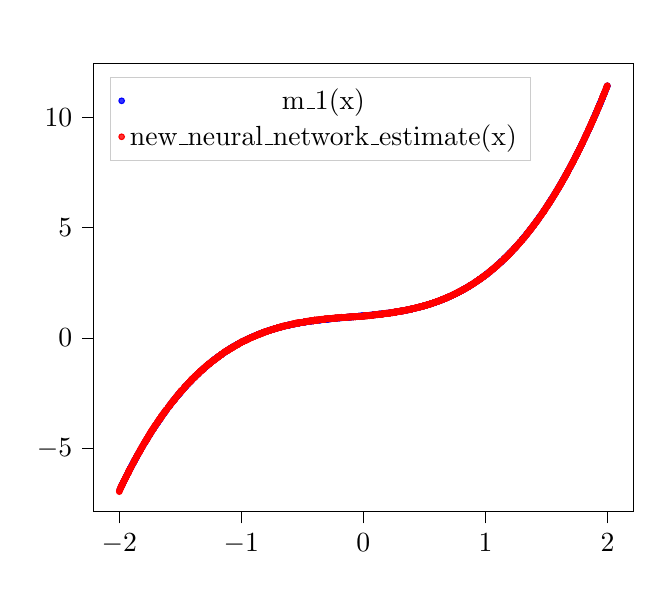
\begin{tikzpicture}
\begin{axis}[%
scatter/classes={%
a={mark=o,draw=black}},
legend style={fill opacity=0.8, draw opacity=1, text opacity=1, at={(0.03,0.97)}, anchor=north west, draw=white!80!black},
tick align=outside,
tick pos=left,
title={\quad},
x grid style={white!69.0196078431373!black},
xlabel={ },
xmin=-2.20852591900454, xmax=2.21306049239568,
xtick style={color=black},
y grid style={white!69.0196078431373!black},
ylabel={ },
ymin=-7.86405361849716, ymax=12.4391808546764,
ytick style={color=black}
]
\addplot[blue, mark=*,only marks,mark size=1]%
table{
x y 
1.98342671961567 11.2067083316341
-0.164883410431491 0.921819789666956
1.40142299960581 5.15033590554207
1.47929179834368 5.7561559124411
1.19715514411127 3.81799531027161
-1.05745151470862 -0.371309570367478
-0.696648319326161 0.464684877420012
1.82247761300943 9.15712037755566
1.33480759235371 4.67626070341997
0.862438587068488 2.32882713322422
-1.16503690445439 -0.754686954628516
0.417168238066338 1.33933090794867
1.15596892097842 3.59120483869643
0.850205757253619 2.28838577184768
-1.30994868597998 -1.39187573215822
-1.55346692657437 -2.82488317686155
1.61669575447566 6.96902026146192
0.500046589667835 1.45907874969249
1.28496886028727 4.34712794233107
-1.20227096727067 -0.904559178268851
0.366681884355046 1.27741420051878
0.818260589820523 2.18688479377424
-1.23845976488916 -1.05920098696907
0.697189507824902 1.8530215419852
1.93926361424016 10.6132554825254
1.04107639834298 3.02636787410901
-0.22353824693392 0.893074337960662
0.668246244317835 1.78431442012492
0.151928097424038 1.08704702436641
-1.07641959705448 -0.433765220730816
1.44298781246897 5.46662361852968
-0.284110387060426 0.860783387392703
-0.44017790192429 0.755901668314636
0.352464522063814 1.26134584362801
1.18574235128237 3.75381711403657
1.66572862979816 7.4485981217319
-1.77196434008901 -4.56390224034042
-1.42077197081339 -1.98366518029347
1.90156609340709 10.1254900733363
-0.399226079743066 0.787289288568677
-0.502642406493864 0.701288589370527
0.570484726981828 1.58079483029362
-0.626439688866295 0.563662303293445
0.646913187691053 1.73622883021686
-1.70011590874738 -3.94019890361793
0.188560902818183 1.11268318790154
0.613581309391728 1.66528403436379
1.53866334933713 6.25708686606659
-1.90745710621872 -5.88963818524853
0.41517370699518 1.33673477925145
0.327838052279217 1.23484812561957
1.73772873954887 8.19951335349887
-1.78984900196206 -4.72748294080677
1.52854808178337 6.16929527049623
0.00832534691972997 1.00418578874098
1.53059984449369 6.18702069900853
-1.45719188829622 -2.19959638868634
0.291257080120115 1.19843927737529
1.19523677300415 3.8071354073554
1.13842913470803 3.49861808490207
1.2366636859145 4.04822570623427
1.89871430519567 10.0892868982552
0.019953194670169 1.01011409945552
1.82122210851877 9.14233718077853
-0.298230517123074 0.852732115538147
0.382945539678767 1.29651503281945
1.08047569362621 3.20916222764976
-0.100962219519459 0.951781416117594
-0.409006788513409 0.780081708579802
1.41020530945337 5.21583204082174
-0.862424320245129 0.156477928786038
-1.98328806650409 -6.72214450231026
-0.696177128652387 0.465406125702621
-0.0933688730806197 0.955318102465428
1.94870249960763 10.73808188061
-0.936123458958722 -0.01976601438959
-1.58312442994531 -3.03409351460663
1.4664267507308 5.65211917053288
1.57141891136512 6.54839610341355
-1.47051135974113 -2.28133185267719
0.874729152014026 2.37035416122943
1.03751084984896 3.01036865668898
1.48030997994332 5.76445750267437
-1.54541524782003 -2.76946312915615
0.552369097636586 1.54760978330716
-1.68042557562017 -3.77839948923686
-1.51061355679375 -2.53657210298722
-0.167528933067055 0.920559140081827
-0.787421015424107 0.310011987252715
1.6501030154187 7.29301335433562
-0.0814367755752747 0.960885772415491
0.0795951024473589 1.04237142562678
0.979738939834169 2.76334381388308
-0.380817770934829 0.800394418604914
0.400591024706831 1.31813698650762
-0.4141113404742 0.776250097560955
1.91403104307527 10.2848760382045
0.920870673865245 2.53445330225573
-1.30315603463426 -1.35866671389968
0.0275601242433647 1.01404829046996
-0.927503900072607 0.00222689952751143
0.0368974953304853 1.01894249538715
1.15977317392 3.61159817433105
0.514097432066963 1.4818167241679
1.17984224265819 3.72104216577677
1.58572120040197 6.6789936011996
-1.37713701802779 -1.73918304115634
-0.472661706237887 0.728589446354698
-1.95506901984573 -6.40446611244112
-1.1779484446276 -0.805616762687941
1.23713048801279 4.05102163809569
0.455615485804151 1.39192818075103
1.59249283776102 6.74155542309861
-0.503448403039978 0.700525301295737
-0.446140509435029 0.75105598593073
0.0961164638478107 1.05196738610277
1.85889095909979 9.59383788518873
0.961953261926548 2.69181699566452
-0.383322867187997 0.79864530138838
0.24213138507616 1.15461989372253
0.788212033700322 2.09669287956382
0.84070370731225 2.25757827157573
1.40004883629895 5.14015179344157
0.107393086597664 1.05870960384272
0.225480591396121 1.14097309250214
-1.67936142766505 -3.7697647231671
-0.0816940927046601 0.960765514872752
1.47773128825186 5.74345186910455
0.401713010033748 1.31954418061981
0.422412491054748 1.34621800253768
0.776700220186323 2.06346076723564
0.317989295994632 1.22470791713495
0.816536031039081 2.18157160974445
1.53962127691442 6.26545353631168
-1.29064269548569 -1.29838208894096
-1.47198666263898 -2.29047742640869
-1.18769903957274 -0.844807189958559
1.5617847179266 6.46159449041297
-0.137017676939132 0.934967618307204
0.10162263173636 1.05523925887493
1.42737547993898 5.34593888574134
-0.755076052164864 0.368829213132414
1.71133977541391 7.91773667028815
-0.4721794317973 0.729011711839228
1.89344301858784 10.0226243465763
0.867958702524959 2.34736672383903
-0.411724457536147 0.778047811177945
0.824378736637617 2.20587035898719
0.170515291427536 1.09977047759294
0.979189264724758 2.76110191698977
-0.897121719560843 0.0767896021307181
1.55034434863224 6.35973527019784
-1.67062801778883 -3.69932121498425
-1.24614106788035 -1.09319208537185
1.54412256063696 6.30489082553266
1.43769151607769 5.42542699235533
-1.6456012323085 -3.50158560570617
-0.635373759957425 0.551982650209956
0.0798070563154254 1.04249250741436
-2.21592582434482e-05 0.999988920530453
-1.56549856175875 -2.90878956620822
-1.85995182081513 -5.40180355705662
-0.744024022342477 0.387963590115266
1.95878262880175 10.8725914329787
1.52876440755115 6.17116216956417
0.252423090403078 1.16334903121843
-0.393738335259513 0.791257880640355
0.449465165244776 1.38318113689044
-1.68386371444268 -3.80637391755432
1.00910500968525 2.88606233001523
-1.12050763647973 -0.587298253264637
0.230997555210016 1.14543091365568
0.0349769356316969 1.01792975394193
-1.56076894216133 -2.87564939931168
-1.45121512537244 -2.16340493618994
-1.16545297771441 -0.756311132410629
-0.0191205019479455 0.990551431326679
-1.86008081192998 -5.4030939017934
-0.436428121653843 0.758911768315441
1.49957184981221 5.9233919160222
-1.44219942190571 -2.10937609184844
1.01529613831035 2.91268092874956
-1.50140183330494 -2.47671254155102
-0.732092139869074 0.408086177914741
-1.31471126281736 -1.41536454673876
-1.16144104543941 -0.740697216143942
-0.689196716081129 0.475997455288745
-0.217022486630988 0.896366930296396
1.62508170186513 7.04925029897457
-0.0406198149252917 0.980157921905294
1.63119848795736 7.1082339788836
0.261617455458398 1.1713441338436
-0.0226785485704886 0.988815972333353
1.93031313461916 10.4958902043135
0.10579027870623 1.05774135817833
-1.34359720927249 -1.56148709026429
1.08272594869317 3.21993898042956
-1.13811010512611 -0.651956813151084
0.157670660808171 1.09091781606985
0.693694852953544 1.84450954897994
-0.413991721747403 0.776340444640307
-0.3496582994086 0.821300655555392
-1.494906796828 -2.43494997466264
0.0812226478153182 1.04330249998073
-1.87946646412891 -5.59912494096078
0.135232078225477 1.07608502949923
-0.0314802740817721 0.984550095861464
-0.536661666154805 0.667662425434589
0.939570817014385 2.6047405093355
1.9606433016915 10.8975565658301
-1.31276353932712 -1.4057380074589
-1.30676601901061 -1.3762731425726
-0.303871457144716 0.849451172880855
-0.643511730589387 0.541119017871324
-0.527466345137777 0.677041842362992
-0.522841202805422 0.681676958703923
0.4944545179478 1.45023449606521
-1.70114092695177 -3.94872752787689
-1.17864666831437 -0.808402179553694
1.70768647325131 7.87932950534975
1.57303031948494 6.56300623145007
0.553581378198257 1.54978869652802
-1.49462820991928 -2.43316685250796
0.0532637575658805 1.02770819278823
-1.03292019870819 -0.293649505337755
-0.0539046615190384 0.973832153044759
-1.4019635634533 -1.87640980895707
0.867566356157913 2.34604301414628
-1.05398034586825 -0.360109127135227
-1.13058478157364 -0.624075386023385
0.588011197017629 1.61419683576319
0.883913094472204 2.40197685981143
1.7032464005838 7.83284702573416
0.723806315564655 1.91984629454512
1.35906175870283 4.84427052411395
-1.23544243096618 -1.04596172691295
-1.54329111912356 -2.75493982502582
1.16098779424438 3.61813290630781
-1.87095954053839 -5.51258428050454
-1.2782629197376 -1.23986916511837
-1.05654172495337 -0.368367143763051
1.24353360832467 4.08955390230973
1.19028282951638 3.7792262679224
-0.775725735545598 0.33177186288789
1.02057273878203 2.93557518071213
0.821921250495339 2.19821881120506
0.918229962933942 2.52470603700035
-0.984864184033527 -0.151361080185913
1.93401749117918 10.5443463915569
1.83315978839409 9.28363700124014
0.533232250852013 1.51399333097939
-0.722014352421549 0.424656658899597
0.481969685265481 1.43090303239757
1.17847167126153 3.71346785213066
-1.79048490297368 -4.73336148187232
-0.945697114342179 -0.0446368331238406
1.60064007186754 6.81744991856981
1.93687669965452 10.5818612825148
1.35197568049207 4.79464642514883
1.91147516287336 10.2520425549434
-0.00460781786329045 0.997702891593491
-1.39948950363334 -1.86251399232994
1.04873511695863 3.06103594471185
0.000913924775346242 1.00045723462595
-0.50513266090352 0.69892519214253
-1.26704247379017 -1.18779508918314
1.76648926011692 8.515401523615
0.157856915922508 1.09104424813471
1.40787527714754 5.19838618820376
-0.240710854768439 0.88424614078834
-1.50153204953699 -2.47755356296565
-1.98239180697612 -6.71190905798603
-0.274480732689117 0.866148734835799
-1.63517535024967 -3.42099958712273
0.960111664862905 2.68452965066336
-0.166975897002565 0.920822887277161
1.54394939093015 6.30336988746059
-1.48090289946801 -2.34614449639195
1.23336476648575 4.02851752917348
-0.400362192403418 0.786460973883875
-1.87413140169175 -5.54475667677901
0.336611711534724 1.24409863604828
1.18872743268058 3.77050370068962
-1.7294971642558 -4.18886360380201
1.45013892943371 5.52266642043676
0.0983398967377997 1.05328401410495
1.82859103308664 9.22936432902555
-0.251038744131117 0.878821858955889
0.0752656353562249 1.03990925556896
0.0812009707648484 1.04329007921359
1.94778947733205 10.7259599229546
1.44701878178583 5.49815477228648
-0.327412551641523 0.835331216623138
0.243300205866964 1.15559974805297
0.092634846159414 1.04991799090477
1.99004222629651 11.2976793178811
0.370987182526909 1.28239482533905
1.12746366204799 3.44192570040845
-0.88103525140069 0.11444499583188
-1.87311208155932 -5.53440536407914
1.53244608154239 6.2030062191922
-0.460133374851041 0.739391819239952
0.307337448869911 1.21402461928519
0.369331774016094 1.28047335921953
-0.234023743918722 0.887711030862566
1.04808634766716 3.05808318471249
-1.71866655486462 -4.09618344887114
-0.541554732849246 0.662580975842837
-1.48954836729529 -2.40077032291578
-0.0346183802921285 0.983037951949156
1.66262513718082 7.41748978740735
-0.0632924638352459 0.969396910959773
0.0976192149694759 1.05285658014762
1.64277341714372 7.22092429870893
-1.23064117143324 -1.02502582306785
-1.2119829712324 -0.945178959503772
1.82543703976219 9.19203877696444
-1.96283859036236 -6.49099090907211
-1.07753916455694 -0.437518252974556
0.401431131407247 1.3191902799471
1.11313051112005 3.36918797402718
-1.82353738645624 -5.04487061859584
-1.02282270803728 -0.262684033496767
1.34249571990793 4.72895418337375
-1.7423388101225 -4.30030535815532
0.574932133692535 1.58914867255579
0.356056594784311 1.26535121241934
1.85225865167069 9.5131424338517
-0.398757442351753 0.787630287557302
0.689987650483266 1.83554534383615
-0.293455390498176 0.855480226380854
-1.36443451041482 -1.67085494806716
1.35065286985791 4.78543213551069
1.01572198192603 2.91452148801636
-1.34644750916868 -1.57624963302143
0.934098979805452 2.58394372921836
-0.337375961698936 0.82913400048838
0.64371991587656 1.72921343065672
-1.12505418398717 -0.603812272410027
-0.0424605535851552 0.97927752676906
-1.03874715299427 -0.311782480194157
-0.934567390971795 -0.0157678258945499
1.06185524551419 3.1213904800115
-1.68614727733944 -3.82501880552636
-0.0939923135416958 0.955027594191503
0.186353265908155 1.1110726428412
-0.702833029741399 0.455143382722217
0.669467597030042 1.78713226709335
-0.989846282352082 -0.16552193374252
0.105206333004412 1.05738943070462
-0.327016013168481 0.835575044028545
0.687399875760051 1.82932776989665
1.84677034716651 9.4467555282193
1.08694083448046 3.24022372148457
1.91270842735118 10.2678755681039
-1.84876330693187 -5.29058235734343
0.140188037147681 1.07929462015681
0.340988226479485 1.24879088314535
1.63241684639954 7.12002930432158
-0.134435062793881 0.936176722358918
1.89935988024498 10.0974738907713
1.10456045506315 3.32642942521779
-0.669863931935491 0.504430082672366
1.20253788657643 3.848623510478
-0.476896000953684 0.72485957082047
-0.864160922436813 0.152624313681391
0.779743629721808 2.07217627840376
0.44847566998307 1.38178594372062
1.88317123466855 9.8936753259772
0.966481764673039 2.70983107632884
0.977908789987251 2.7558871775324
-1.52375847203518 -2.62327699740979
1.13406912530685 3.4759673999773
0.522353840992912 1.49552708713273
-1.06822671124227 -0.406527917387101
-0.114355250680581 0.945546284394021
1.89308302690468 10.0180838654405
0.845248577878253 2.27224791568968
0.122425695926454 1.06795770242727
0.127977871489443 1.071452329096
0.01625186865687 1.00821615648482
-1.08796984143618 -0.472845104422563
-0.320666677251147 0.839450527601591
0.334320179485394 1.24166256257872
-1.05886861846269 -0.375902385164731
-0.564026324025872 0.638414711051878
-1.59115775979802 -3.0921520343033
-0.624686875303529 0.565923843870914
0.0413789150922659 1.02131826057146
1.31657491972719 4.55336406862912
-0.726992150093075 0.416520105094092
0.0524606842524733 1.02727218818635
-0.492141039700758 0.71109076518107
0.978275827209485 2.75738082493985
1.14130644500639 3.51364516032462
0.0392796360480538 1.02020313016701
1.30721738204172 4.49141064784605
0.490133920204322 1.44348012355915
-0.706442978901193 0.4495096644889
-0.993964710262591 -0.177329563835979
0.943620152780988 2.62025423675144
-0.0932557921766692 0.955370798670078
1.6365425027311 7.16008680515812
0.973324880119798 2.73730832363678
-0.725054451856926 0.419698555277889
-1.96417313354495 -6.50592462133396
1.31324497867966 4.53123083543522
1.87324432504556 9.77024625410757
0.303189087378309 1.20994224416354
1.9389374422235 10.6089613728723
0.501357612206841 1.46116901188386
-1.720056540905 -4.1080112039577
1.31781128519504 4.56160630738453
0.0951516110926338 1.05139794858651
0.408192815810979 1.32774813968817
0.513811453765586 1.48134650425401
-1.23574332705072 -1.04727912774199
-1.45264147142963 -2.17201479615298
-0.227918340918484 0.890843932569515
0.768794189473504 2.04105392984846
-0.383261040749235 0.79868859764658
-1.52535647365474 -2.63392131109938
0.978901900798691 2.75993067808586
0.989417826238432 2.80315006002761
-1.36387886985462 -1.66789491236366
1.30076519383918 4.44913205476502
-0.61920844932297 0.572929632714456
1.33769433552972 4.69598515376487
-0.74829966725375 0.380618179060386
1.65991412952015 7.3903995937643
-1.54882463937474 -2.79285887150011
-1.89409203935268 -5.74981453952136
0.116957207902192 1.06455795146663
1.17623321690576 3.70112896015788
-1.35372154548933 -1.61420715774001
-1.88141472578473 -5.61905888338989
1.32924807506156 4.63847962469226
-1.77134487512033 -4.55829675676622
-0.128741369799476 0.938838418393211
0.51095333379939 1.4766641046124
-1.67747670266001 -3.75449901365524
1.29669044236686 4.42261577546358
1.34952912501012 4.77761666284377
1.33266062176777 4.66163835456556
1.12465453846378 3.42754849841394
0.4823513930431 1.43148567258717
1.56244015327284 6.46747005636869
0.11081670699023 1.06078907799291
1.47420921577403 5.71486476538048
-1.40118206014657 -1.87201510170116
0.634664924286693 1.70957467919594
-0.684074619393981 0.483658496059001
1.60007325210646 6.81214767306192
0.871416435428499 2.35907231047904
-0.983390175523971 -0.147197135538043
-0.681323886845001 0.487734387895415
-1.26150283611157 -1.16241909746674
1.67379753998392 7.52995968901337
-0.987930545268803 -0.160060852020812
0.454921140058064 1.39093417506421
1.51394338581359 6.04432436735546
-0.804954691722807 0.276317438492785
-0.830724433208845 0.224398470191638
0.335858029439155 1.24329584466934
-0.159847298344431 0.924212755588489
0.0812119985668653 1.04329639798377
-0.117494185355901 0.944084196411911
0.497555841122187 1.45512515695177
0.640924836877307 1.72311134065059
-0.123471924446762 0.941297774124052
1.15598732778889 3.59130324256049
-1.27272624906405 -1.21406008321854
-0.76949998857843 0.343125991938706
1.4162089827075 5.26101451251004
-1.91041766129389 -5.92088694414514
1.99504962001563 11.3668989718006
-1.00490416987749 -0.209143338340367
-1.14258809682261 -0.668718416842979
1.18209823855401 3.73354181514181
0.128884868780194 1.07202738126087
-1.94570137893154 -6.30108914105676
0.27471991687839 1.18306806252273
-1.72671969673579 -4.16498229116897
0.187211122317864 1.11169743641647
0.48198115722144 1.43092053557093
-1.98132421803257 -6.69972954213555
0.758502825129475 2.01238871783111
1.34931125357486 4.77610269536153
0.245180659219023 1.15718232866859
-0.276183458320058 0.865207129827379
1.39456510983045 5.09968311504284
-1.6804327463332 -3.77845771215393
-0.665754239595305 0.510306575023814
0.76684140612743 2.03557122891776
1.09948744175177 3.30137507524853
-1.7534846008282 -4.39840634527731
-1.83044998652393 -5.11151071125484
1.37370201959309 4.94821688942207
-0.382340179934817 0.799332698920512
1.84016263074689 9.36729469457565
0.288068510119739 1.19542452478037
-0.114543656857639 0.945458542257138
0.206795309294432 1.1263285058384
-1.57769003775003 -2.99515593056534
-1.03763955741927 -0.308320801104982
-1.52268760032851 -2.61615653065817
1.11941760456987 3.4009040701208
-1.33311090638393 -1.50771004489711
0.128759478350397 1.07194781107472
-0.202242477740643 0.903731634603166
0.878360806223666 2.3827980126127
1.19855610565421 3.82594465441631
-0.95885680090605 -0.0795950750614648
1.9731762658412 11.0668248504742
-1.30507394687268 -1.36800862623331
-0.0157669575178914 0.992193314134026
1.88887607888191 9.96513724318019
-1.01174714032224 -0.229379091520865
-1.56039182316205 -2.87301570032441
-0.926950247777248 0.00362671646421875
1.64418618486032 7.23477519532048
-1.20043385996112 -0.896947485134618
-1.59792808416967 -3.14154749994605
1.69730156795686 7.77094735900795
0.575625029518244 1.59045760970327
1.4325210476095 5.38546272461785
-0.821655978972185 0.242999595633413
-0.810842030128184 0.264710330683507
-1.76436741471195 -4.49543613243629
-0.101373628416222 0.951589874479197
0.645687235329547 1.73352993640201
0.10576329327991 1.05772508508171
0.497152732945724 1.45448746150772
-1.20605108820682 -0.920293170938932
1.65818341412337 7.37314604751803
-1.87962426988887 -5.60073796632451
1.33566435853625 4.68210715495086
0.282054103858054 1.18980470698956
-1.26250466931175 -1.16699204691647
-1.67476380995526 -3.73258686461563
1.01967995195807 2.93168806191011
-1.67840964447672 -3.76205118380057
-1.50130451410046 -2.47608408679851
0.141109062399635 1.07989515924757
1.20995178365977 3.89118827835135
-0.531511081284835 0.6729432404821
-1.54006889061477 -2.73298567027789
1.66007705123738 7.39202540581725
1.38566787929341 5.03460666896519
1.42172807729341 5.30284416594051
1.19501735684592 3.80589515622314
-0.0613276058947694 0.970323119939249
0.588196574174466 1.61455706145536
-1.86528429810381 -5.45530051391384
0.327998076046251 1.23501500011517
1.94392556510098 10.6747725129444
0.391687289083808 1.30710792726173
0.953213581470196 2.6574299461252
-0.727575792369922 0.415559950077793
1.21439774087505 3.91692509422767
1.65999716563432 7.3912281841227
0.382087929756178 1.29548822962649
-0.16287160981814 0.92277676837371
-0.0542029915768536 0.973690800842405
-1.63260596193285 -3.40129984579709
1.12690113690572 3.43904191500925
-0.602201080415101 0.594083125950106
1.26792747852857 4.23945539583106
1.30847145779741 4.49966965275129
-0.718738337998323 0.429960531379342
-1.86119536711375 -5.4142508988663
-0.356727609725149 0.81669094026702
1.90459290272936 10.1640216503881
-1.44227588332194 -2.10983146250815
-0.391557970599605 0.792819909722158
0.631524958158446 1.70285186854789
-1.8673507757779 -5.47611714719273
1.42661454192866 5.34011495936151
0.170205151974584 1.09955348313825
-1.83568026427185 -5.16227865205378
1.2073940863486 3.87645422732492
0.706156293104354 1.87513804754791
-1.98203177551578 -6.70780014014512
1.36502793573962 4.88639889620432
0.399224089177922 1.31642786191096
-1.0253447363566 -0.270364174212614
1.50929202137678 6.00496342833847
-1.63337973901535 -3.40722582261244
0.16217533939344 1.09399145885371
-0.98542617423463 -0.152951737923894
1.5360467607192 6.23427976294006
-0.483081925171916 0.719337382260632
-1.58770633174206 -3.06713467478903
0.754998431678347 2.00275622643676
-0.315694310614774 0.842448548232049
0.80731770988626 2.15345551594596
-0.520999610898754 0.683507318681412
1.49195497855709 5.86011399750875
-1.10514956412394 -0.532465223812011
1.97857357935404 11.1403174392499
0.201904204556214 1.12260731318804
-1.48063273802369 -2.34444782161577
-1.74765842069912 -4.3469663733447
0.97582411111886 2.74742059343922
-1.94025775141107 -6.24148801641387
0.378690645694897 1.29144231745017
-0.675642050925532 0.496069283877749
-0.85135959252331 0.180704325857191
1.29651347872175 4.42146741003185
1.38442162021466 5.0255486562329
0.0993659004083431 1.05389365645253
0.322056803667919 1.22886488173402
-0.319240158445763 0.840313911505586
-0.584549292170264 0.615110609184494
-1.12598759652605 -0.60721864335168
1.41262589486618 5.2340088706993
0.646121632266878 1.73448545340135
1.78052185613418 8.67289265981815
0.0456857711294889 1.02361857502653
0.650561123062864 1.74430075452423
0.444925785300273 1.37680795769407
0.360910773533672 1.27082206027476
-0.00804773722748919 0.995996648292271
0.377237311240174 1.28972199915939
1.52091849859923 6.10374749026291
-0.0373496792893628 0.981725351704962
0.862206665085895 2.32805217881156
-0.507190355652468 0.696960910121683
-1.86205179057238 -5.42283330831689
-1.70459448861946 -3.97754027439972
-0.151804594967045 0.928017392461753
-1.68436080041345 -3.81042813744005
0.187659122172576 1.1120242490766
1.3554496588658 4.8189190431175
-0.487869327729311 0.715003204906045
0.842675192251204 2.26392694634303
-0.912200762028982 0.0403535280591013
-0.946369416514677 -0.0464010410197027
0.330462441073498 1.23759349000862
-0.0195847733926913 0.990324603273036
1.26237990986932 4.20493049782254
-0.675334511443002 0.496517206261075
-0.229399784212416 0.890086353839939
1.9604831935885 10.8954066810646
0.653098747548911 1.74995226855662
-1.99271462098377 -6.83038081816128
1.52604705488264 6.14774493496474
0.265785713873526 1.17503120638017
-0.162967637142707 0.922731122134607
-0.283790790788197 0.860963045149854
-1.36121907666447 -1.65375883389091
-1.31329929847602 -1.40838314891627
1.81527813187679 9.07259527626234
-0.442821583254181 0.753762240778201
-1.35568360263731 -1.62451551362428
-1.51220574381476 -2.54699354010741
-1.88865198249977 -5.69348252498278
-0.0584710604719203 0.971671561732019
0.381577876562059 1.29487859540097
-0.606990213147065 0.58821653307224
-0.749626560934504 0.378324034734459
0.00894689778701219 1.00450019527111
-0.134416985656438 0.936185181356841
0.947482538246278 2.63514997624858
0.652193660151404 1.74793312291132
-1.4971053276791 -2.44904543319222
1.73588142591092 8.17953815015466
1.82488208996298 9.18548319269702
-0.433621813289647 0.76114591416293
-1.85764198404764 -5.37872869313915
0.189957707840087 1.11370674618603
-0.0839730204312175 0.959700875691003
1.24728831958757 4.1123056418777
1.65468022478909 7.33832011275106
-0.586495676362482 0.612837325483901
1.79589799743536 8.84802129209566
0.428791423729258 1.35471550491822
-1.21645298698983 -0.964090333743602
1.5431165224241 6.29605904121035
0.178665194044994 1.10553169571189
-1.65418653612307 -3.5687317524992
1.59677966307949 6.78140367909103
0.933307944837329 2.58095305728585
-1.77917297787843 -4.62942925053352
-1.02449591391644 -0.267775315313738
0.586894557125167 1.61203007076959
-0.522527848756777 0.681989010527291
-0.839039065755164 0.207022944691082
-0.985881123675554 -0.154240675866536
-0.464749211709719 0.735452035855211
-1.64426334947883 -3.491186075905
0.467548491374151 1.40927248703334
1.92460116275829 10.4214987297265
-1.6443087962847 -3.49153905651549
-0.491293941305216 0.711870026008429
1.91222188641349 10.2616270266605
-0.62453546156841 0.566118745447308
0.300401507594917 1.20722329431868
-0.408259673873164 0.780638446049794
-0.386727514305038 0.796251031923926
-1.2807629327012 -1.25159562141562
-0.35007346853807 0.821032011779048
1.81278321825848 9.04344311739489
1.04336477412012 3.03668320841017
-1.32183939999296 -1.45083724437438
0.292077450222015 1.19921892546656
0.994071082116497 2.82251080980646
0.177466744750081 1.10467731384257
-0.505717794748531 0.698367674676974
-1.43761031855531 -2.08213415727262
-1.89149919300563 -5.7229237053933
1.28583777853235 4.35268374821217
-1.68115385495103 -3.7843153794068
-1.4142254050391 -1.94600789683803
1.52526984373002 6.14106061529525
0.612917731722653 1.6639222092179
-0.607365102169935 0.587754345462488
0.0446778208985652 1.02307869555183
-0.96209360813814 -0.0883318304875763
1.30375431185376 4.46867408429554
1.44134726467672 5.4538346503775
1.00844224545156 2.88322832443489
-1.59164327974008 -3.09568014470601
-1.93898777050765 -6.22763304253179
1.75462960692508 8.38402365592018
0.409361680989284 1.32924207079661
1.96570363363382 10.9656676715992
-1.89042953048247 -5.71185225186763
0.634605413505302 1.70944684791535
1.51117328592788 6.02085759885574
-0.336130600952831 0.829916161502131
-1.70081948401835 -3.94605184186047
-1.17900918117107 -0.809849619160207
-1.88055737118247 -5.61028146583971
1.7226892869659 8.03798589758147
-0.28444331034676 0.860596119807494
0.256235525537556 1.1666413705637
1.70534277107545 7.85476685433527
1.12385801800205 3.42348268523638
-1.47077804764093 -2.28298371381439
-1.61806822565318 -3.29102278955293
1.90294759424218 10.1430630966633
1.44451129494468 5.47852266160623
-1.01616478290891 -0.242580965266955
1.15493317240572 3.5856718757953
-1.40498242439259 -1.89343221858113
-0.452277827687501 0.745991134070497
-1.02618668656894 -0.272936092067389
0.16135892421457 1.0934319415492
-1.38881021937692 -1.80309489411771
0.83749527307802 2.24729452697683
-1.50103564033491 -2.4743482179168
-0.486808076009357 0.71596857791788
-0.538027218351843 0.666250669752277
1.9974166483278 11.3997283821791
0.0678536146367503 1.03574211366182
-0.0899177932002528 0.956926814390687
-0.427960738075485 0.765604944431546
1.60332836723081 6.84264236473997
-1.91821035570889 -6.00361962545922
-0.484358263630535 0.718187066115336
-1.14455694548876 -0.676128497006041
0.0304102520839233 1.01553439168116
-1.35890685005729 -1.64151467560062
-0.79930465921805 0.28731719612153
1.73862147320117 8.2091801257019
1.45803599732521 5.58511646755393
1.89547191274214 10.0482431762309
0.690931727750082 1.83782178852227
-0.621921289478656 0.569472296962388
-1.85804910216955 -5.38279143389878
-1.90519163173854 -5.86579373854702
-1.16833564944958 -0.767594943367109
-1.97462737655031 -6.62363958121218
-0.318014178865605 0.84105380251823
-1.6721081152242 -3.71120685604103
0.12506651417845 1.06961442749644
-0.598865775068001 0.598127669210699
1.77408588270415 8.60038455461797
-1.28722274061527 -1.28210603288769
1.97264479348539 11.0596075319345
-1.38334936445139 -1.77306192632327
-1.4234852858919 -1.99937517996845
0.68138823441224 1.81500941674427
1.04276100159047 3.03395800254456
0.363443058450483 1.2737027863533
-0.484681708491861 0.717894959660252
-0.42417904656689 0.768548456579527
-0.463869516349239 0.736206471705505
1.51603821310448 6.0621205930325
0.758851818256217 2.01335155326038
-0.361724413726992 0.813386601010214
1.9077891816332 10.2048298360685
-0.325593495457903 0.836447991161261
-1.4194697586773 -1.97614676213254
-1.98060600755018 -6.69154355462185
-0.74386957637504 0.388227584497721
0.0550760056004314 1.02869441717498
-1.07639607264541 -0.433686442070373
-1.98146995411248 -6.70139135895703
-0.614558293171367 0.578802301776621
0.580519533847571 1.59976104188703
0.85530197722539 2.30512646438327
1.16025561474269 3.61419236913617
-0.856557722320832 0.169393066404631
-1.15325753072591 -0.70917200147902
-0.239167870624584 0.885048828266123
-0.763721926225796 0.353522802407235
-0.977358490724609 -0.13027982803673
0.778036169125887 2.06728038238241
0.884340845547061 2.40346215552389
0.328138275778158 1.2351612579192
-1.55099225540116 -2.80778775223326
-1.03940188301237 -0.313832078552333
-1.72324163505083 -4.13518796186514
-1.84654800214979 -5.26872481567198
-1.43760044903241 -2.08207575751688
1.33241634702983 4.65997723453523
0.00470785624302161 1.00236123791202
-0.756956890576916 0.36552483747915
1.47817407575479 5.74705420485713
1.7488753934927 8.32084679314365
0.24029622852773 1.15308731260398
-0.229712543158756 0.889926204763276
0.936394382750414 2.5926445628988
-0.588247452495922 0.610781821734327
1.12089743121385 3.4084122555828
-1.68973056641353 -3.85438000159527
0.601490598378976 1.64077414366491
0.485060318584069 1.43563571921682
-0.743511201112161 0.388839796458524
-0.237997845978876 0.885656203601219
0.465159036576552 1.40575968640309
0.221364441760389 1.13768751303374
1.84453390617883 9.41980429808891
1.00647655101298 2.87484055951728
1.01000925130016 2.88993373969193
-1.87754777380837 -5.57953526649142
0.768807495091131 2.04109135728871
-0.126510324543307 0.939880107966774
1.59224876657191 6.73929233360148
-1.96901747277081 -6.56031066024765
-0.151585860600471 0.928120599126281
0.27514404486757 1.18345419050871
0.928969564002895 2.56462168594107
-1.13912071298838 -0.65572847467495
-1.3946007413604 -1.83520004087116
-1.53647125544187 -2.70858343004002
-0.853899259225281 0.175193415056966
-0.168066577292175 0.920302623347891
0.80680243856385 2.15189801728073
-0.568715904490896 0.633195480283646
1.90853719763859 10.214397764992
-0.788490064341025 0.30799463717303
0.442582735811799 1.37354566431466
0.459054233603626 1.39687552247798
0.39261749399079 1.30824877454604
-0.334717090759574 0.830801289010195
1.94086803536182 10.6343968181273
1.72074136428306 8.01724701749925
-0.292636510585159 0.855948854822363
-1.8825587450258 -5.63078399959954
-1.44751382991273 -2.14114206316334
-1.66380916147449 -3.64484099058998
0.401861302912721 1.31973046275312
0.623271629065938 1.68539340121019
-1.73144970591821 -4.20569915378075
-1.77371702050308 -4.57978392318897
0.955956320015098 2.66816793758185
-0.18897993598519 0.91023036546916
-1.6234885758441 -3.33190439423898
1.09818757474448 3.29498592215778
0.309124261139459 1.21579642671328
-0.0852514379276199 0.959103955205731
-1.20296402390791 -0.907436646342982
-0.270626161478439 0.868269331607198
0.580911905551383 1.60051121866171
1.89911009192989 10.0943055577833
-1.064461094195 -0.394142474879605
1.01285946066994 2.90217317390131
0.0402853617909917 1.0207368752534
-0.721932674649874 0.424789386080467
-1.66297073792276 -3.63817368047019
-1.81194227253934 -4.93425282463376
-0.65222601397195 0.529244626005021
-0.471450844379962 0.729648654986886
0.0370646534067927 1.01903079271421
-1.40749154055525 -1.90763621540311
0.695183252394338 1.84812752899872
-1.3887485131105 -1.80275420632957
1.85291059689277 9.52105182117024
-0.357923961782797 0.815903315065873
0.974884463317879 2.7436137850711
1.09839082028482 3.29598410091773
0.830736918330413 2.2258271038816
0.470309061762373 1.41335589628585
1.72836875306984 8.09869154159071
1.46857383792811 5.66937208921194
0.456457372499913 1.3931356304433
1.66877894800176 7.47927364775083
1.39834539959636 5.12755138331202
1.56275324449412 6.4702782522399
-0.325545359330059 0.836477482958752
1.85992830537649 9.60650597509558
-0.723639418786876 0.422010679340869
1.94494266655738 10.6882289495346
-0.603203955844345 0.592860405091233
1.7499954109815 8.33311478767895
-1.54049166796916 -2.73586090180703
0.259609595491829 1.16958206817038
-0.731632112601908 0.408851007811368
-0.0519325411599803 0.97476729017708
-1.72438866505661 -4.14500022640276
1.5064929250508 5.98137889887683
0.887629961378167 2.41492021599477
-1.11507085610526 -0.5677200891142
-0.917751339073211 0.0266596159564805
1.59838189136926 6.79634572283596
0.0866958965644469 1.04645605141118
0.511077028010305 1.47686610904852
1.18267057389016 3.73671928077183
-1.50837712909309 -2.52197132499597
-1.11106653271358 -0.553417700758948
1.81148448128094 9.02829616101279
1.50251810418365 5.94801949158777
0.814115306622483 2.17414199110334
0.790250422365434 2.10265274415143
1.63443981901696 7.13964875211235
-0.233454491645942 0.888004345247047
0.586663233387293 1.61158186572004
-0.0497866633920321 0.975786287788734
-1.61536089253957 -3.27070757076436
0.848178812923249 2.28176978444151
0.245000662573484 1.15703051541659
1.53488813686981 6.22420253630332
1.36834242044437 4.90994069397324
-0.704148960054754 0.453095256084725
0.00630860309351045 1.00316749235806
-1.40491432443655 -1.8930474153221
0.829387278753886 2.22157156070566
0.317830262660781 1.22454626287515
-1.90365540241397 -5.84965805885858
-1.62753556811879 -3.36260966263985
-1.07974178139327 -0.44492376214492
-0.0401652628917479 0.980375534538642
0.860426038380392 2.32211294404568
-1.97271544571729 -6.60201419432597
0.190591970662848 1.1141726925123
0.737104817700763 1.95457775769123
1.79080319347672 8.7896957865979
0.180385991615295 1.10676284928859
0.269402073604749 1.17826216971268
-1.21119745824843 -0.941869770922104
0.452501685883913 1.38748350398462
-0.672242667744425 0.501002119019167
-1.87624541070442 -5.56626179799371
0.697491518131789 1.85375997540669
-1.20317623202471 -0.908318352432709
1.03305973959424 2.99052061568452
1.93968190507009 10.6187642477155
-0.821861577213577 0.242581884621014
1.63669141219185 7.16153596429626
1.12811869078702 3.44528671234127
1.18993959765328 3.77729979941787
-0.25536082126297 0.876524214114186
-1.53401697010337 -2.69200261869658
-0.179743031420164 0.914703026826147
-1.02306687395788 -0.263426005993494
-1.74238098504039 -4.30067414845448
-0.468060562638022 0.732596940922769
-1.52858752321493 -2.65551241532027
-1.66643863626171 -3.66579564315443
-0.641421382308617 0.543930131873093
0.538245752971836 1.52265960139125
-0.955234916781065 -0.0698838993363239
1.80447172410411 8.94684189758768
-0.263185865738656 0.872320671481494
1.20310768144324 3.85187921672936
-0.759262351682819 0.361455230000449
-0.100655606763484 0.951924170797343
0.395716018306588 1.31206807179805
0.87211821829841 2.36145681851321
-1.15580354177307 -0.718933512086722
-1.46536166469255 -2.24955290054648
1.48295138677626 5.78604032278067
1.61459884644588 6.94907314634342
1.12568219517709 3.43280119124754
0.866338688902824 2.3419070079037
-1.88149196370742 -5.61985003530082
0.796995975427856 2.12253861289157
1.18993904227527 3.77729668298541
0.00326378068726907 1.00163538782081
0.99147879094986 2.81170713649919
-1.16854127436226 -0.768401909148824
-1.41411347488116 -1.94536708041133
-1.18129361556432 -0.818990900220248
1.75555598117783 8.39422907605019
1.4068679209575 5.19085919088058
-1.11794299148175 -0.578039886374277
1.35976299670166 4.84920562717139
-1.62864042117664 -3.37101946941616
0.837123791554514 2.24610769688773
1.90712812877881 10.1963798514224
-1.04264993613093 -0.3240363185946
-0.899533795903042 0.0710358364792234
0.131443054211328 1.07365571281068
1.58641001943151 6.68533601707391
0.133184681131325 1.07476973412852
-1.66808451108402 -3.67894626701431
0.958140299087838 2.67675334517056
-1.20071553721398 -0.898113080369225
-0.29853548062793 0.852555704806701
-1.59020194748787 -3.08521285924393
-1.14679993698604 -0.684600564244047
-1.80395518812676 -4.85889899518877
-0.137678202125405 0.9346581819364
-1.47745500338493 -2.32453774310355
0.939519736387501 2.60454548209869
-1.35213428522258 -1.60588969662356
1.55564777901188 6.40679070736085
1.3123367672864 4.52521084209601
-1.00625054930137 -0.213104313097389
0.22162258394559 1.13789256241124
0.480912021948272 1.42929135626533
-0.400866712337033 0.78609239569891
1.49035524462727 5.84689554278936
0.160235802126708 1.09266401209588
-0.0716438000134736 0.965470942110219
-0.888570383890701 0.0969612511986682
0.982840776990081 2.77603261006682
-1.69495795594223 -3.89744184996925
-1.4617497943475 -2.22739769747757
-0.42314483375042 0.769348589512897
1.59181588354367 6.73528003652307
0.591841901406039 1.62167046929035
-1.93229760790966 -6.1549561757401
-0.306711411046629 0.847784880556625
-0.138148433919949 0.934437841218547
-1.26896132597228 -1.19663623420301
1.68454711978169 7.63943621503765
1.1392782281719 3.50304601511557
-0.480386448395481 0.721754395289265
-0.490322690457073 0.712761417952586
-0.275439661364084 0.865618817515639
-0.54345663381348 0.660588689748085
0.613200605364189 1.66450249809784
0.688492804968752 1.83194973760757
-1.21377118055488 -0.952727981570386
-0.290464321290868 0.857188260010645
-0.477369279494698 0.724440156259689
0.527679401870274 1.5045097951213
1.52837326464824 6.16778693077292
1.31999322543593 4.57618457231067
1.49828207824019 5.91263737722987
0.141132714179094 1.07991059789785
1.27727139459846 4.29818992337106
-1.31957472473445 -1.43952592683124
1.07403596830212 3.17852442267588
-0.964152382379572 -0.0939174689590342
0.372903814950484 1.28462951769261
0.338964532666234 1.24661469892759
-1.90283120211612 -5.84101222823902
-0.538926179282687 0.665318605805233
0.640452057593696 1.72208273447832
-1.79462195146616 -4.77171112771805
0.845175689742974 2.27201170294667
-1.12367227739812 -0.598779210451571
1.38580255251099 5.03558633887015
0.781039940610238 2.07590383792586
0.742219428079976 1.96817826018767
-1.19406467829478 -0.870734118277661
-0.0449801113196626 0.978074598174748
0.632269387643565 1.70444168365252
0.95299971641987 2.65659470437528
-1.67434856904174 -3.72923934056497
0.295928098180434 1.2029004453019
-0.626471885314217 0.563620670988828
-0.214640428951248 0.897563375662694
1.14999846380373 3.55942407415894
-1.69462783017563 -3.89471430687958
1.00236726771143 2.85739090847459
1.63395337111733 7.13492709980748
-0.823298339067957 0.239657661120865
1.32830160638183 4.63207459559869
1.04968038564894 3.065343494382
-0.872053718616644 0.134932772431856
-1.35649547964011 -1.62878970674586
0.437074209182266 1.36594863663831
-1.95504569295756 -6.40420740716794
-1.08877311971084 -0.475592819257362
-0.490078402446558 0.712985271015062
-0.0849870563214972 0.959227383047594
-0.835507401722747 0.214440962342617
1.15150322718474 3.56740809740603
-0.348840406187581 0.821829140042039
0.32956554445898 1.23665318101434
-0.634505395875966 0.553129141425036
-0.712102981416007 0.440580147511722
-0.141181527238492 0.933015530624069
0.480824629828942 1.42915836771712
-0.993803048145222 -0.176864334335354
-0.350082585525117 0.821026109561412
0.516649780001659 1.48602722259306
-0.5906743819141 0.607919149502502
-1.38542315227203 -1.78443923472196
0.0552461398158584 1.02878717007279
-0.160301599759029 0.923997242450794
1.61316880277441 6.93549586466522
-1.01829581720307 -0.248988405125319
-0.605550343710735 0.589987699174208
-1.13095129953082 -0.625425045182286
-0.430802229699371 0.763374751301627
0.481892362246438 1.43078507028784
-1.3585046072138 -1.63938887888464
0.738234268448013 1.95756946471052
1.01394446821935 2.90684705473204
-1.41398252492884 -1.94461750198599
-1.61322129466368 -3.25470147546836
-0.652286033515564 0.529161966391323
0.933830736067949 2.58292913135864
1.43087486679923 5.37279130342767
-1.00525884447349 -0.210185800461815
-1.50577099100418 -2.50501195390687
1.69439119087545 7.74078341437282
0.10925386070688 1.05983790235327
-0.188831907928934 0.910302370929738
1.57725839578374 6.60146623821642
-1.65640169917705 -3.58617255705754
-0.0101443338755236 0.994960212353824
-1.08708920938024 -0.469837268188092
0.441869766673601 1.37255664793776
-0.564949950927475 0.637391656904085
-0.823574016021408 0.239095543015953
0.174998644970009 1.1029256423352
0.35957055618162 1.26930486866708
1.01517511591745 2.91215807920767
-1.01068379458088 -0.226217569950526
-1.01107275652972 -0.227373296108133
1.59442120696011 6.75945724907352
-0.345592888348411 0.823917773481681
-1.29280590229753 -1.30872129958885
0.908709804141768 2.48992821737328
0.251582943895579 1.16262780597153
-1.67068398963368 -3.69977029502073
-0.358884765262246 0.815269170072609
0.543566188111855 1.53196512814761
0.39052183014819 1.30568228138866
-1.78482711120297 -4.68120920110513
0.392427898563614 1.30801603114462
-1.75534148417263 -4.41487490434709
1.8503004408122 9.48941536715725
-0.919870775031479 0.0213903298721088
1.47400951506076 5.71324744708682
1.75263123441605 8.36204118570609
-0.198501908355358 0.905574384373035
1.30090062834669 4.45001583074007
-1.66407712761412 -3.64697335799929
-1.84703443163292 -5.27351959062834
0.849949429186349 2.28754778244004
0.212031550491898 1.13036315308368
0.328070932321069 1.23509099799962
-0.76219608701357 0.356245856880229
-1.05034528540007 -0.348455087434208
0.130191110209795 1.07285764383031
0.238265181418163 1.15139947479866
-0.1604445162542 0.923929431107584
-1.88544272017285 -5.66040746381983
-0.355263481040195 0.817651875296108
-1.62197081642769 -3.32042900348838
-0.27260628005381 0.867181855396237
-0.0393374727000664 0.98077204637976
-1.67029587641437 -3.69665697078896
-1.4710559598251 -2.28470574025771
0.3082855060622 1.21496370491836
-0.172468446827101 0.918198235346273
-1.34416057620319 -1.56439999322047
-1.33564904373112 -1.52064952502959
0.802023719528068 2.13752419665797
0.59189749511968 1.62177939336193
-0.325807182637529 0.836317032850372
0.929845640955968 2.56790994971066
-0.220918870588491 0.894401548446393
-1.71225608825882 -4.0418882790471
1.8403591192216 9.36965021921371
1.12938560758863 3.4517965635835
-1.5047675750776 -2.49849804363137
-0.861877904777332 0.157687562511912
0.613015809930273 1.66412336752378
1.99783392103624 11.4055229812418
-0.600432925376096 0.596231459695451
-1.45190828144078 -2.16758691243222
-1.48904013730822 -2.39754134298098
-0.285818161709389 0.859821491004982
-0.440240268030195 0.755851362680721
1.94114199811838 10.6380099391004
1.5203777216456 6.09912332861589
1.42674268688303 5.34109535400439
1.53771130486377 6.24878063047949
1.08882233533862 3.24932053509569
0.737204249571775 1.95484086941443
-0.658852549666758 0.520045515942364
-1.56974238807888 -2.93869925768835
0.573850104841899 1.58710864281915
-0.150629813670606 0.928571540966119
-1.59348005323711 -3.10904716797659
-1.78069008218441 -4.64328957281517
-1.23127998733112 -1.027802140198
-1.22026092161847 -0.980308555640824
0.882795537168005 2.39810156317915
-0.930186148595834 -0.00457659538527411
1.79227171174474 8.80647713121272
0.766752410763582 2.03532184929355
0.773207551344699 2.05352048702182
0.260074786136564 1.16998950568125
0.252140468136878 1.16310624064939
-1.14290600744467 -0.669913248840446
-0.374213118765592 0.804955680857456
-0.191181658633414 0.909158058002845
0.810589974522598 2.163381259695
-1.41514599508773 -1.9512822678602
0.395078496897364 1.31127984273892
1.16524505127672 3.64112744273495
-1.03632649241488 -0.304226042565756
1.18948005796077 3.77472198587331
-0.270297527364671 0.868449433874931
-0.198422000604987 0.90561366269916
-0.857131906047643 0.16813602458199
-1.47168682695009 -2.28861721392019
1.30970381039638 4.50779879595879
1.08896952136146 3.25003325106136
-0.253744816342775 0.877385261341134
1.60809238143707 6.8874700276336
-1.46164224840128 -2.22673969804884
-0.523674976294005 0.680845431379947
-0.436105436776697 0.75916946927637
1.95670181580846 10.8447229790432
-0.29578081090816 0.854145237454634
-0.146498271875552 0.930517489092381
-1.48114813660415 -2.34768518142267
-0.360618287314252 0.814121407141682
-0.137969553008917 0.934521666109314
0.692041230923785 1.84050269395564
0.848541326972606 2.28295127115617
0.306602934648166 1.21329862270282
-1.99440478525603 -6.84990030388248
-0.163046902412025 0.922693441264199
0.807028705077833 2.15258176473391
-1.38021215283323 -1.75591511891502
-0.391259388345681 0.793033169097501
-1.28762850152753 -1.28403263820684
-0.174382470327815 0.917280783766521
1.13131840297683 3.46175128155318
-1.37045581518671 -1.70308653950514
1.88195365105748 9.87847330015004
0.42451589737284 1.34900533570564
-0.250619191395958 0.879044006890007
0.203502318902969 1.12381816913033
-1.58694498485549 -3.06163097800262
0.506640548475837 1.46965705070567
0.74023425649113 1.96288327802345
1.21036770304808 3.8935892176777
-0.783689800415043 0.317015675037404
0.36004969780675 1.26984669049933
-0.00841423401782704 0.995815284654669
-1.36225289641879 -1.65924676348695
-0.169846151402795 0.919452780658226
-1.80167404054627 -4.83750329606028
-1.71064649794186 -4.02832064119088
-0.0144324412344345 0.992848406647661
-1.71446370448892 -4.06053936154386
0.588542852677619 1.61523034349259
1.69359471543941 7.7325445269266
0.960172150386684 2.68476864465872
-0.501004418258892 0.702834934789813
-1.73543242629262 -4.24016056347248
-1.18738325377207 -0.843528056777747
-0.784046358824987 0.316348896817618
-1.41258173898454 -1.9366078844798
1.71385367062331 7.94424996569319
-1.95982876404981 -6.45738784953313
-1.74772858892011 -4.34758380647548
-1.8435030868594 -5.23877001754084
0.662633333223705 1.77145552470409
-1.97857398165206 -6.66841640626697
1.46737028666602 5.65969553365888
1.40820450129305 5.20084818512847
-0.26203923453244 0.872940237525545
0.446314292887601 1.37874996770754
0.423303278566297 1.34739667713506
0.654264776554472 1.75255916982409
0.195648317957575 1.11791351216775
0.869789244443124 2.3535548140646
-0.972812372591263 -0.117657788190493
0.728326427169269 1.93154966766546
-0.615050256398702 0.578184193752807
-1.68378682359237 -3.80574701635623
1.32645410070877 4.61959452246244
-0.00306303876824643 0.998471500496445
-1.92613251195332 -6.08844338856703
-1.7678595137034 -4.5268330652448
-0.294710498461862 0.854760461822923
-1.4156965362227 -1.95443979345889
1.73060191716862 8.12265833310048
-1.19280754552839 -0.865592394287253
1.31589340472998 4.54882640739453
-1.20936667062426 -0.934173394631358
0.824988959339324 2.2077756649389
1.44994772354708 5.52116167829113
1.66091128157801 7.40035470103932
-0.822159008525746 0.241977269724585
-0.783898941357204 0.316624637232964
0.535165215213903 1.51732290557903
1.37416286857846 4.9515201528893
-1.26707642429524 -1.18795128714585
-0.594686170782149 0.603148756327027
1.50327056291737 5.95432281026179
1.92323778364012 10.4038007624767
-0.0661064161920821 0.968072202724847
1.7973699615765 8.86492744905595
1.78822759931664 8.76032265014644
-0.0355696491027953 0.982580429304874
0.710778270422538 1.88669431924725
1.79510199198771 8.83888910864229
-1.6013204280294 -3.16645825549723
0.827550060828212 2.21579542506338
0.710290387126795 1.88546942765681
0.75328106345806 1.99805941204832
-0.602679413986287 0.59350031537745
-0.736116787059058 0.401360263426038
-1.75442056855673 -4.40670289919965
-1.43469212012865 -2.06490171684732
-1.42457901983685 -2.00572488115273
-1.85067490959863 -5.30948688938268
-0.356802885485278 0.816641446786753
-0.483117331157287 0.719305522849883
-0.737512856820079 0.399012610082135
1.93790301004031 10.595351464905
-1.21266198885831 -0.948042898510603
1.53227608060943 6.20153286471949
0.94099363195935 2.61017957606926
-0.00887345133348605 0.995588151009568
-1.15415909725177 -0.712623858434803
0.591980211072964 1.62194148219783
1.36550586974274 4.88978744815124
1.70357448545846 7.83627435027178
-1.70289120626857 -3.96331499568938
-1.40104805470438 -1.8712620281133
-1.61851806470054 -3.29440499476517
-0.63112002838442 0.557575573319032
-0.565084838129248 0.637242049113841
0.851954413494163 2.29411277330813
0.48982569862781 1.4430008972904
1.45141946350045 5.53275280275556
1.29955424466575 4.44123700840332
-0.84757109003723 0.188870428958125
-0.0599663634505343 0.970965410863567
1.24627519307932 4.10615513282809
0.778027223959338 2.06725477506621
1.11303740065966 3.36872048346061
-1.07369452877235 -0.424661437034536
-1.06772890975252 -0.404885801541526
-1.61984117288767 -3.3043641509849
-1.56478897897108 -2.9038045844714
0.935177122726119 2.58802629462615
-0.511888877383642 0.692436685658468
0.453053721775183 1.38826905851069
-1.10552539167778 -0.533789646913369
-1.82968366491081 -5.1040974467213
-1.66590564833054 -3.6615427251593
-1.92322212449706 -6.05719723651022
-1.64755790625506 -3.51682616610233
0.536198102612343 1.51910810086017
-0.107249325761568 0.948854634668092
1.96901847512502 11.0104557393676
0.223121280965427 1.13908566639894
-1.70559709939951 -3.98592738382609
-1.25120198878827 -1.11581428511409
-1.86325846684435 -5.43493952243064
-0.117696588412903 0.943989897472763
1.82415943911388 9.17695190231721
0.562110201979332 1.56528687742743
-0.560464756988403 0.642337358042499
1.36413404164186 4.88006667367168
1.85764949536136 9.57869371898181
-0.572732680065321 0.628675610461671
1.31909501625392 4.57017833613826
1.31768933845374 4.56079275955768
0.953529119384244 2.65866280935027
-1.62428029635491 -3.33789907091573
1.23452868466645 4.03546076426489
-1.22147326342045 -0.985492891674448
1.32006706182028 4.57667862051968
-1.75140090095866 -4.37996875561887
-0.879055494390023 0.118993780269021
0.54827145310572 1.54028869924352
-1.03646261797876 -0.304650088505529
-0.29642091653693 0.853776665310185
1.69965456488001 7.79540165753882
-1.92626251476466 -6.08984139395354
1.25754503364581 4.17505045600754
-1.39510351177812 -1.83800024057679
0.768149445576419 2.03924146447786
0.629209199577733 1.69792232313776
-0.398388833061027 0.787898226117644
-1.85205832248426 -5.32319312482858
-0.788306477157378 0.30834141495755
1.92336307531936 10.405426230607
-0.70940929986311 0.444844585697191
-1.62290632240129 -3.3274995398133
-1.90084325800046 -5.82019063857491
1.89309179361197 10.0181944192673
0.470274000325968 1.41330386505985
1.62265830770733 7.02598987553108
0.893485980468911 2.43548364637751
-0.733495310758882 0.405748290948773
0.148485290971542 1.0847514676653
-0.150844352111013 0.928470370725297
-1.91783695783904 -5.99963945317911
0.190400907466076 1.11403225548728
0.399679743270707 1.3169969369697
1.096754005881 3.28795402126858
-1.49633334111525 -2.44409122497096
-0.958128006818784 -0.0776354898908592
1.98316190841294 11.2030781834086
0.235138767152799 1.14881836851237
0.159138615959582 1.09191580441678
-0.50351942722194 0.700457964971038
-0.747017559231104 0.382828317131004
0.954233168495334 2.66141598552957
-0.984114947122056 -0.149243088442066
0.566261707929518 1.57293847659294
0.0268518303870944 1.01368001238554
-1.5080912666153 -2.52010818864839
-0.698445924122061 0.461925923461316
1.55686017968182 6.41758757741351
1.93469424921284 10.553216972581
1.53776104519807 6.24921437317124
-0.862739132584211 0.15578038107934
0.79029759576884 2.10279094050976
0.0471274247975035 1.02439239875053
1.78987721790029 8.77912690052206
-0.0431857369949249 0.978931048381096
-0.929862394078688 -0.00375346834793933
1.92044127119492 10.36756965867
1.65432556888321 7.33480166918088
0.33085216554685 1.23800274922351
0.70593915826521 1.87459777061375
0.529588679409994 1.50775701177613
1.15961162919433 3.61072991364129
0.927783599136133 2.56017804399492
1.51679446472447 6.06855578095598
0.505843770609108 1.46837017949939
-1.86608403340888 -5.46335098835564
-0.13183306760037 0.937393734241051
-1.5948633922361 -3.1191350481614
-0.402491431752823 0.784902332976656
-1.2133053277603 -0.950759255996364
-0.399992927369038 0.786730451090819
-1.12793902639114 -0.614357814757456
-1.81371503806416 -4.95107099648
0.999099306135273 2.84359567367731
0.252238154701149 1.16319013979868
0.724810795768328 1.92243806366124
1.35877053448433 4.84222226357485
1.44383629208362 5.47324790942361
-0.52201647213084 0.682497725271347
0.792357051294308 2.10883613132269
1.13142344393241 3.46229309621455
-0.909827386308057 0.0461623830673111
0.627588348397961 1.69448642159623
-1.66249879225256 -3.63442369352429
1.0244559071169 2.95254617827994
-1.06115849580953 -0.38334870945599
-1.08590118719238 -0.465786940173083
0.547207888067801 1.53839951004046
1.52819489594 6.16624825942774
0.638538035700954 1.7179289325443
-1.4204616749999 -1.98187240908629
0.966847435128181 2.71129155995665
1.75335340411573 8.36998004208666
-0.502963356595071 0.700984834758228
1.93133594447325 10.5092527985002
0.538941134559069 1.52386945789964
0.188749750665735 1.11282136647531
-0.292593598496842 0.855973391432946
-1.37039122070766 -1.70273926532393
0.102400835197629 1.0557047712163
-1.53332126060227 -2.68731226056737
0.891235759838326 2.42755720186516
1.52170743807571 6.11049884802857
-0.844376562263295 0.195705543756215
-0.375488262401924 0.80408067223377
1.4696309220224 5.67788246054487
1.13816047065756 3.49721817323933
-1.84272956088872 -5.2311765844534
-1.74749904667497 -4.34556417819544
0.644838063213352 1.73166457646492
0.482666975213408 1.43196777559443
-1.89561475321412 -5.76564239081856
0.0640935205283264 1.03365067786788
-0.993936303270147 -0.17724780418363
-0.182062122929765 0.913583883048714
-1.76248041563369 -4.47852345492373
1.6180302702965 6.98173882657229
-1.72862303592487 -4.18133915761499
1.26946417620312 4.24906447899531
0.0232857615563313 1.01183199442652
0.376062841662597 1.2883363499593
-1.92558451797562 -6.08255259910049
-0.301932119684734 0.85058343404128
-0.615330242664868 0.577832079638759
-0.574937648601093 0.626174929312303
1.24780110159707 4.11542187846027
1.62037688557016 7.0041481320128
0.776891640072805 2.06400746289965
0.805897067176439 2.14916497188128
-1.04699449756928 -0.337780348737123
0.2413457555599 1.15396291866958
0.779938874450223 2.07273712296313
1.05148057441272 3.07356436028159
-0.60208950984249 0.594218965773506
-0.662847385953129 0.514428181055222
1.47783716222536 5.74431304459151
0.677094877773097 1.80489057535815
-1.36138557463422 -1.65464211025583
0.826952051915089 2.21391948052634
-0.616460223808683 0.576408519698541
1.90049331762246 10.1118598699591
1.8857421665975 9.92583229362722
-1.99232133463139 -6.82584373830562
0.347339572283597 1.25569397803319
-1.94164832298215 -6.25668016754697
-0.87580042214737 0.126432453372567
0.618131148387185 1.67467389041367
1.64951506747112 7.28720973548482
0.856870484129805 2.31030965843759
0.75816365172245 2.01145359287336
-0.630893720992384 0.557871496703937
-1.68440412323232 -3.81078159312989
-0.801909424927161 0.28226301307832
1.67684929108731 7.56091329136224
-1.77823002811071 -4.62082666321174
-1.50476161515709 -2.49845937961117
-1.07092277187912 -0.415446994640916
0.554453463411948 1.55135983180469
0.343066363886576 1.25103729993777
1.78407551388253 8.71312912961346
-1.04397837982574 -0.328227301390198
0.562222038737691 1.56549207455857
-0.866328340604409 0.147795038857713
1.25613287223244 4.16635985946709
-1.90746279943368 -5.88969818106689
-1.287035879447 -1.28121919610003
-0.539949798500574 0.664254689315366
-0.862636863904048 0.15600703402093
1.01478429583278 2.91047031699819
1.23975984222251 4.06680364423564
-1.19235655588129 -0.863750409325774
-0.831963437570925 0.221828798485852
1.40265973241274 5.15951629228891
0.0194303791313675 1.0098453788844
1.40372315003464 5.1674213568491
-0.528505640610852 0.675992745163049
-1.6564367176555 -3.58644865323731
1.69314550365526 7.7279008288673
1.18427001205538 3.74561264251057
-1.49048114937126 -2.40670243203198
-1.5021541457011 -2.48157349939488
-0.973580992960761 -0.119784081701067
0.780153688626938 2.0733544205084
-1.97175917019071 -6.59121430968625
1.70812572752589 7.88393967866811
1.71164628801791 7.92096566685086
-1.46901377285881 -2.2720670262631
-1.23705343296793 -1.05302246946098
-1.31701534670063 -1.42678900543212
0.973916433523538 2.73969810519761
0.0138870558554998 1.00700893829624
1.24736888638784 4.1127951120542
1.85797901316208 9.58271162347587
-1.55414649990604 -2.82958745285144
-1.26664102180807 -1.1859487335488
-0.491671869592991 0.711522572045034
1.56608847925319 6.50025427042704
0.106986326153375 1.05846356533392
-0.524782636566406 0.67973800984612
-1.28628653522886 -1.27766539355675
1.96238202836105 10.9209239716033
-1.51631884062425 -2.57401806958537
0.649325034600645 1.74155870983148
0.724807417907873 1.92242933945989
0.0888190227673209 1.04768881497555
-0.727130728089694 0.416292246427935
1.61375447966397 6.94105389685173
1.85902495714243 9.59547356068222
-0.26205808636835 0.872930061358466
-1.91095938475336 -5.92661571731319
-1.84063806586138 -5.21067802010906
-0.83203390035015 0.221682455008366
1.77395758284144 8.59894387399551
1.39522424578815 5.10453286882605
0.991061263606985 2.80997126875214
1.75867999543365 8.42871557387581
-0.145078200731571 0.931185345721736
0.424811330532875 1.34939798162108
-1.97676835775563 -6.64790737169224
-0.0224534136102359 0.988925588632502
-1.79084339270371 -4.73667740838314
0.623736702573969 1.68636904571803
1.74134746699276 8.23875263443377
-1.22329593745987 -0.993306226618697
-0.68863543648969 0.476841503255705
-0.841565476998836 0.201682049751289
-0.114665665274081 0.945401721077095
-1.27052530195143 -1.203861842856
1.78013467986155 8.66851747260619
1.86228752760561 9.63536391582172
1.54718747645037 6.33185935875192
-0.0767255669261084 0.96308944111748
-1.35816488303435 -1.63759446223621
-0.494991410247095 0.708456202517538
-1.45696110771646 -2.19819336995244
1.06594787433349 3.14046823450914
1.93612990897787 10.5720532579514
1.90943433588774 10.2258819915518
-1.45262100952012 -2.1718911615037
0.785661940921628 2.08926897040826
1.48129203807223 5.77247401344108
-1.78019018746414 -4.63871983208713
1.95664099860872 10.8439092498593
0.477914979210265 1.4247462952397
-0.515843724751158 0.688586128698253
1.50482410118571 5.96735421244212
-0.434201139132909 0.760685999633963
1.09245878750959 3.26697566808596
-1.35868571455372 -1.64034585027071
-0.758148874059312 0.363423392727458
-0.786945539293618 0.310907702980332
0.52878601489933 1.50639014501486
-1.63848464065965 -3.44646537614018
1.36992278408109 4.92120022086491
1.61674374079115 6.96947727260168
1.0830007265137 3.22125744692358
-0.492413148033551 0.710840088759813
-1.06776075633125 -0.404990811139046
0.349569286229697 1.25814391282824
-1.76802641988979 -4.5283368888717
0.454907214792726 1.39091425702831
-1.90638792522486 -5.87837759132325
-1.54731497238487 -2.78248642605251
-1.43140345060785 -2.04556579019779
1.81777930286695 9.10189243174927
0.0749928195697884 1.0397548078862
1.89915503061025 10.0948755081904
-0.456716963407882 0.742278124899361
-0.831663785685692 0.2224508961276
-1.21310084781679 -0.949895577925508
1.56068431452565 6.45173980936193
0.918894025714693 2.52715306974637
-1.51902640644904 -2.59188884866268
-1.85715800237426 -5.37390130183896
-0.19956111548409 0.905053393591488
0.127893873663956 1.07139913277355
0.78402794741665 2.0845307395796
0.808996478858507 2.1585402118705
1.22984588684676 4.00759330424166
0.234445791603679 1.14824903644456
-1.2782780393036 -1.2399399481654
-0.609232095571956 0.585446173369471
-1.03990220203699 -0.315399958059745
-1.63056543630134 -3.38569990115128
1.67575051841743 7.54975703877128
0.790850052170221 2.10441029419865
1.43535004703875 5.40729800660216
1.28305857717661 4.3349362174954
0.602211871837049 1.64221837714499
1.17002221696631 3.66709775231917
-1.96969016459752 -6.56788478965851
-0.420503314401308 0.771382845430355
0.00566025559792926 1.00284072543611
1.68187917657893 7.61214922970133
-1.32969440699063 -1.49036988534212
-1.21559370058737 -0.960444327997432
-1.51750003742957 -2.58180640932343
1.78995853088708 8.78005459910523
-0.533564886410108 0.670845822719905
-0.863322864649673 0.154485756564612
-0.485369859142183 0.7172726778564
-1.90882702469775 -5.90408524932761
1.41520006110501 5.25339829886051
-1.35924644196202 -1.64331034841882
-0.861356600799521 0.158840316600257
-1.31755553564965 -1.4294732040879
-1.11214461415033 -0.557258553461082
0.383861508736479 1.29761414507274
1.41257472447696 5.23362405936077
1.66732817080819 7.46467150976683
0.315562558070873 1.22224832688126
1.15482684194415 3.5851043270083
0.883803781254541 2.40159746566727
1.34039284239157 4.71448965561803
-1.96618885461039 -6.52852077074172
0.520093164339951 1.49174708496151
-0.059431820558177 0.971217772926455
1.20056066320666 3.8373461174504
-1.26527759983197 -1.17968671330802
-1.19603151765713 -0.878799840768772
0.908964190174309 2.49085015515867
1.64444117719047 7.23727740584927
1.83226136004263 9.27294537353598
-0.618081054980039 0.574359623139687
-1.79611021553569 -4.78555162805232
-1.45813243987457 -2.20531905080718
0.0797175808956805 1.04244138701734
-1.68602571107216 -3.82402493587793
-0.83913379187387 0.206823209072277
0.369839788247009 1.28106217047193
-1.96293142430682 -6.49202905123444
-0.977438612004603 -0.130503269498393
-0.764717547176466 0.351740938790488
0.665388103370584 1.77774792956026
-0.95405496559106 -0.0667349281815306
1.74365110010926 8.26380751553717
0.88937319263139 2.42101968929262
1.44053858124633 5.44753982488186
-1.06214485291108 -0.386565669563593
1.61677967387832 6.96981950711904
-0.969711271564239 -0.109110859264739
-1.10111582664108 -0.518304852801946
0.479358068620247 1.4269307348515
1.00147119269776 2.85360105200195
-1.50614978008554 -2.50747323363271
0.135087463666287 1.07599192289944
-0.10437397163449 0.950193113552419
-0.865024945595861 0.150701782569106
-0.227882217765365 0.890862384696654
1.74774498479461 8.30847914790494
-1.06749011983779 -0.404098616506272
0.447194619714659 1.3799846034777
0.191706917504417 1.11499353633612
-1.53467718360765 -2.69645765329396
-0.0303931324022266 0.985074991992057
1.97064170860828 11.0324372794247
-0.338622466202244 0.828348925746348
-0.763123127650191 0.354592550778447
-1.78187740239317 -4.6541539279079
-1.76095886117017 -4.46491322418032
1.05509605695447 3.09014445357528
0.471792586686954 1.41556143616822
-1.63713799322961 -3.43608993064268
1.21639985543668 3.92856695231781
-0.209052526897512 0.900355406759493
1.17052390765357 3.66983542516921
-1.68780168124837 -3.83855902194721
-1.3546328996739 -1.61899157436293
1.48663823198821 5.8162777913109
-1.65635437320755 -3.58579944386302
-1.67608702535521 -3.74326547549861
1.21350843499642 3.91176433969345
-1.87888741434495 -5.59320853108333
0.395408335680854 1.31168749807443
-1.79419211586412 -4.76771815281607
-1.51250302176874 -2.54894179033519
-1.61684686950874 -3.28184943102874
1.58631980276513 6.68450505598533
-0.802594996628898 0.280927956280322
-0.0794859431731667 0.96179783037884
-0.732966009715986 0.406631070533624
-1.01893260734773 -0.250907994009945
-1.63790006061609 -3.44195925555662
-0.615478446559309 0.577645597833662
0.343695035731867 1.25171922039455
0.57779178361288 1.59456375401596
-0.699937440091468 0.459627865535633
0.707100514414448 1.87749020069058
-0.886972889362756 0.100690569025272
0.815133489524867 2.17726293510365
0.764683353719457 2.02953595477432
-0.34376078044843 0.825089264565482
-0.335400168623273 0.830373901387892
-1.60973235621782 -3.22869365261734
-0.0625530951816025 0.969745318511178
-1.56187486241968 -2.8833802995486
0.235851754428173 1.14940519024992
-0.604510140635392 0.591263300128981
-1.52595209584025 -2.63789453670762
-0.0167539530500709 0.991709448812335
-0.48133754314143 0.720903460043628
-0.331574810527902 0.832758980354371
1.11301569467954 3.3686115109984
0.26433173410415 1.17374059837321
1.86404601882561 9.65691630769074
-0.351661789064046 0.82000187970048
1.30528355617809 4.47870152488599
1.13849983059223 3.49898654693974
-0.700254175629474 0.459138814559712
-1.16323425742782 -0.747663206520722
-1.09317503071268 -0.490719432982972
-1.50947056014758 -2.52910445464645
0.369611341071494 1.28079729679421
-1.93280424225842 -6.16044165455544
-1.58252649628825 -3.02979597900591
-0.763232969381421 0.354396427529145
0.697362563986819 1.85344461974421
-0.78885638453812 0.307302274213614
-1.97001006573632 -6.57148858056276
0.41282324688506 1.33369168895236
0.0915867832461297 1.04930396860131
1.38481369648395 5.02839681198353
-1.37682768681298 -1.73750406988822
-1.81277009698659 -4.94210215315662
-1.5436799434384 -2.7575953075135
0.31214230664009 1.21880760764692
0.745415545892666 1.9767462646854
0.908678008631643 2.48981301339038
1.58766883354634 6.69693929600202
-0.115972246424081 0.944793175590471
-1.77203737735337 -4.56456341357926
1.99893935864718 11.4208845267762
-1.08983879770738 -0.479244124305624
0.606564105436654 1.65098108377588
-0.59347945779573 0.604588689282053
-1.75972116339784 -4.45385988010386
1.41433405500788 5.24686843839027
-0.565038180623414 0.637293804248749
0.629341526646942 1.69820335474672
0.359092699084816 1.26876515243835
1.31209455722298 4.52360657942307
0.0231655473192554 1.01176987386168
-0.91855554467885 0.0246628562726551
1.76618437749433 8.51200436784866
-1.88883365455313 -5.69535834021965
-0.35877884193425 0.815339150943887
-1.28223361298719 -1.258515120528
-1.74717176179298 -4.34268550251242
-0.0381931754896185 0.981320627546728
0.28756260071101 1.19494845761518
0.149413701940852 1.08536867189767
0.408579070397023 1.32824133588349
-1.49914779368727 -2.46217781434149
0.0744843979020424 1.0394671982087
0.838133071460148 2.24933406340543
-1.25106277067889 -1.11518956498603
-1.94527337085676 -6.29639042233159
1.63989670287326 7.19278579532602
0.947947137930402 2.63694823975164
-1.95022300713495 -6.35085915138298
-1.14036041717668 -0.660364012151103
1.59891211959265 6.8012963388368
-0.557883632982971 0.645158125220656
-1.90969707059121 -5.91327184497705
1.08206173751063 3.21675416302705
1.34230080876573 4.72761185919997
-1.36304571536481 -1.66346099869758
0.198751080498258 1.1202323785615
0.0171134301767624 1.00865701431544
1.09076257328937 3.25872843042728
-1.22084344547998 -0.98279834030487
1.95397912147747 10.8083379921804
1.84483292780524 9.42340441154085
1.90754866825673 10.2017548388507
0.988413745574071 2.79899146699252
-1.16113479370591 -0.739509628040418
-0.898757806765679 0.0728899639194056
-1.72453369303265 -4.14624182096285
-0.218035835765646 0.895856789997443
0.269600038029095 1.17843990359055
-1.78591422979284 -4.69120367724842
0.658024340641895 1.76100770281471
1.80974732277935 9.00806624621475
-1.40394985040404 -1.88760160308266
-1.50873158780901 -2.52428253507125
0.307451961694163 1.21413792736538
-0.528884650568429 0.675609467041245
1.4386350581012 5.43274695287675
1.09033381004139 3.25664705752175
0.522694119614134 1.49609776021739
1.54715171273416 6.33154412831436
-0.669302419702281 0.505236420592782
-0.59255965317619 0.605683348425251
1.52492262642214 6.13807633920665
0.309944458185623 1.21661245618531
0.494040954130513 1.44958500461109
-0.721085446062989 0.426164658692831
-0.695056255808788 0.467118618177397
-1.07749284575177 -0.437362833929012
-0.791133218524787 0.302986357719246
1.53796642661311 6.25100558859299
-1.03394103954002 -0.296812271055293
-0.559812087764417 0.643052368011132
-0.633968339936727 0.553836990474224
-1.08897230869268 -0.476274773578637
-1.83406499079466 -5.14656803373782
-0.815162051023353 0.256098168103319
0.143125881657654 1.08121468711607
1.22397845948015 3.97292829861374
0.725829322232748 1.92507132628676
1.3715998567677 4.9331732876944
-1.52342357214668 -2.62104908437208
-1.93042075917092 -6.13466094661306
-0.616595189844368 0.576238222099196
0.213993461034763 1.13188857365299
1.39803812909352 5.12528131282752
0.100701243153916 1.05468909117862
1.35925049059371 4.84559833145911
-0.554927920621903 0.648365664774076
1.97667711505462 11.1144531365842
1.57800292613626 6.6082575605031
0.645395105646288 1.73288784568775
0.974282898146801 2.74117972496166
-1.03708996103011 -0.306605699392774
1.69454522744885 7.74237759001367
0.375377173129433 1.28752927895184
-0.655548801477311 0.524650300775287
-0.953868870865906 -0.0662389530943418
0.282829356831491 1.19052423629332
1.34300982734016 4.73249637214456
-1.17640153921017 -0.799457174811928
1.18335643107566 3.74053038779944
-1.58585802253435 -3.05378273525992
-0.406269387633428 0.782116550369699
1.64426823954281 7.23558031363243
1.8751683113906 9.79407752265142
1.6271576806091 7.06922491586328
-1.41956760269503 -1.97671119129604
0.91561499477998 2.51509692453709
1.42657150446897 5.33978572828725
-0.226384349697887 0.891626661442817
-1.37240178410673 -1.71356383293874
0.329503820648372 1.2365885486861
1.76835687279365 8.53623420599155
-0.0643571965988285 0.968895435777672
-1.04472205333709 -0.330577886582466
-1.54851585294466 -2.7907356294578
1.74531312125836 8.28192067639441
-1.29753201911022 -1.33142964625767
1.03058135477804 2.97952910077753
-0.739307202417413 0.395984147242487
1.07074212816424 3.16296938985897
-0.276871417668281 0.864825836028826
1.59428070989477 6.75815166865391
1.9775394033217 11.1262076505164
-0.322668723171736 0.838234307567092
-0.755764004994456 0.367622206163626
1.65383353457481 7.32992254260252
-0.144282128392698 0.931559525911121
0.402805096754445 1.32091764161098
1.24507461810011 4.09887761868257
0.735468533287763 1.95025524288497
-1.64111697855334 -3.46679688829703
0.0579891524950362 1.03028656200424
1.67760140437525 7.56855725419944
-1.69368273555164 -3.88691181889737
-1.24377755022998 -1.08268901549638
-0.432681352834765 0.761891095706417
-1.35297342057784 -1.61028445695437
1.92355852750648 10.4079623031266
-1.57448990466284 -2.9723539336749
-1.34222151991915 -1.55438427031929
0.289194162205326 1.19648599819658
-0.286787433879757 0.859274129623031
-0.656062103608636 0.523937269374979
0.536164444597334 1.51904986165716
-1.22738074864422 -1.010899981434
-1.29505040068755 -1.31948533683892
1.26892424565769 4.24568599818437
-1.92474243500583 -6.07350719887432
1.55085128086431 6.36422090095643
0.680577102095658 1.81309088302144
-0.298382311684437 0.852644321350996
-1.65984865582475 -3.61340658154561
-1.68973754295019 -3.85443729120498
-0.899730465091301 0.0705654553515266
1.79002475993214 8.78081026076583
1.24563099265532 4.10224871154197
1.57497112340899 6.58063788084533
1.37769729650331 4.97691775303615
-0.281410350029088 0.862297708674295
1.93491822661699 10.5561539738156
0.0363111485001473 1.01863296478277
-0.332987432240669 0.831880589168509
-1.80974006411356 -4.91340769524829
0.694896077357561 1.84742862080097
1.95457147794537 10.8162462688562
1.27308420348949 4.27177908733688
-0.874512743956169 0.129361319704098
0.914187743108128 2.50987033058807
-0.244938422010026 0.882036783630122
1.9907673585679 11.3076838361221
-0.13346042304654 0.936632714681418
-0.68233701334333 0.486236293949049
0.548963450448359 1.54152031847289
-0.808553351871949 0.269240248340317
1.04654601741391 3.05108454552819
-0.119795110934064 0.943012023037743
0.701049984621372 1.86249454770044
-0.226734136952503 0.891448333304594
-1.43358458674436 -2.05837995413147
0.374885551613246 1.28695146707067
1.68338246621681 7.62751502901291
    };
    \addlegendentry{m\_1(x)}
\addplot[red, mark=*,only marks,mark size=1]%
table{
x                      y
-1.52762947004398 -2.63665679852607
1.74584146706459 8.30313418504723
-0.523478826928232 0.684981455327291
-1.73063347132838 -4.16754055824511
0.199724526357971 1.12413986692501
1.56583537106678 6.50212130573281
-0.463057519114948 0.747665654157118
1.27292037122199 4.25911843213007
-0.561300740541583 0.653996446870297
0.640763194967071 1.72674751050313
-1.73791342939199 -4.24096264611894
0.131982542924304 1.07163562445192
-1.83168405496555 -5.10376196338133
1.09632486787013 3.28860190499629
1.14869409291258 3.54804856022076
1.71062342784982 7.90152466385944
1.54063884052671 6.26233498072305
0.96036949117845 2.67188471681226
-0.36582225744249 0.829228691385662
1.03292095360504 2.98417928381415
1.57196496539069 6.54609386202508
0.316383914894403 1.23104885644691
-1.25339289598648 -1.13554910601212
-0.46394682067964 0.740299643711383
-0.998800252147865 -0.168876133428104
1.03613462412239 3.00699952570108
-1.64532444822729 -3.49293200198847
-1.97015264204063 -6.5769121469698
1.10611827964268 3.3325927944455
-1.40144531975216 -1.84518158676689
-1.71485775358785 -4.06883587132901
-1.55651601432609 -2.85466248166607
0.704149753887608 1.87137436411416
-1.35391349938216 -1.62114783985896
-0.19713428931697 0.91320639815536
0.890553629834266 2.41963800191651
-0.748635890255846 0.367757908994129
-0.0825495453396563 0.955542429515598
-1.52863234199303 -2.64905992413016
-1.06308264251695 -0.412431701954534
1.34829445246638 4.75822063973227
1.21677724541683 3.93402096649771
0.321064511493674 1.22796917544757
-0.79448963572049 0.286639405408638
1.29306522904297 4.38129536324555
0.991145476362639 2.81469205516578
0.408046183683614 1.33070158460102
1.50470887336654 5.9575393202239
0.241965856580386 1.14976159314043
-0.698625089638838 0.462631462074469
0.69277772759134 1.84475566662164
1.54249469168855 6.29223000018984
-1.37940963447366 -1.77397785165444
0.328552328283534 1.2358697609747
-1.76899063762277 -4.55181464197594
-0.1615118341785 0.917358084831994
0.979551973019646 2.76474222344531
-1.41400818915192 -1.93743608707598
0.920422122884637 2.5371272327229
-1.58813906344299 -3.08034023934407
0.567973302168688 1.574798756124
-1.7027550272339 -3.92661639975712
-1.66143052087379 -3.6310451778419
0.509387499079396 1.46884150329936
-0.649372469635067 0.531357119197573
1.27714939756953 4.29644865621161
1.99062920502101 11.3301714102496
-1.77767653093197 -4.60832173114591
0.95231808494159 2.65334945903267
-0.729339734657573 0.394415405360015
-0.69929992108586 0.469586842821553
1.62359205741297 7.03622721245334
-1.26350376928392 -1.15873251814128
-1.80495773362803 -4.87445067342779
1.4755075644755 5.72000202565798
-0.582140577898955 0.62882666918393
0.391595936124218 1.30969317341825
1.68359095958506 7.62901889841519
1.55014341230999 6.35669199872224
-0.461713591692503 0.760474080303689
0.837995109576847 2.25388599012062
0.0647111588263334 1.03231598849297
0.449501515148342 1.39080169134864
0.842450703096236 2.25731626328023
-0.662607691037783 0.514319433635468
-1.73347656811602 -4.21427270283707
1.97125407913951 11.0374500899417
1.06434018406928 3.1398766859045
1.24774144636567 4.10652488237163
0.301552235654667 1.22610695051265
-1.419054264094 -1.96851225748391
0.770735380506118 2.05529699022521
0.673663615667701 1.79826450863936
-1.20717318186629 -0.921117900268635
-0.410538504386376 0.765068471502614
-0.997783575545104 -0.190561556633821
-1.9247004506919 -6.06488872678494
1.67307707998314 7.51858011026587
1.13094409339522 3.46594756951591
1.05978614977254 3.1119281304365
0.368497683846726 1.27437039746974
1.19041117219778 3.77115160864485
1.53532876144759 6.21911480195912
0.977879415140715 2.75127965038619
-0.661130676558663 0.515515881624548
0.372560417149814 1.28014251982014
-1.41713935044321 -1.96759316741115
-0.721990537872462 0.427308795775999
-0.593304843043549 0.610478409782568
1.39782862521232 5.11259491405215
1.31945403787629 4.55774479220443
1.29797173081997 4.42915493648867
0.500221801881652 1.46197989702367
-1.22858048710803 -1.00927000019683
1.84901594258915 9.47648534922581
1.5150131259747 6.05407785409292
-1.22889583462019 -1.02559434722004
-1.4115062222231 -1.9348610640109
-1.33406864789987 -1.49095685339282
0.212784793779644 1.13119633500023
-1.35572868353146 -1.63622217917435
1.34923257581794 4.77328323295919
-0.117934710702453 0.944959877079549
1.74259492028609 8.25448605318237
1.79584748839092 8.8397486108736
-1.56683538172848 -2.9161474951396
-0.100670899179379 0.954539281248498
1.3130637409383 4.52476010808466
0.413802060319139 1.33744361353339
1.03952918317515 3.01003625023142
0.355758361430128 1.26871554742047
1.06587471434403 3.13952285378779
1.47827077764151 5.73417393797497
-1.423248862284 -2.00477990059306
-1.64138318843414 -3.44920568469485
0.858985773610331 2.31055719751639
0.30940079900652 1.21678960560482
-1.59532819132151 -3.11544889268605
0.674828392358402 1.79411719788582
-1.99791465316728 -6.92318765043389
-0.983915817371269 -0.150434192007041
1.05210422602657 3.08040038211607
-0.460520520996104 0.753445163781151
0.793577616390077 2.11102106409086
-0.916701943346689 0.0293686277642946
1.80568436851851 8.9740041455143
-0.41905914986584 0.775491286151664
1.4905136786334 5.85347534864318
0.659003889297849 1.76823560366373
1.33264972737708 4.64719307545267
0.367019067455185 1.27683076268824
0.284838881991474 1.19735122698525
-1.56586227893797 -2.91574117100978
0.865300493711527 2.33095887814049
-0.939391307968867 -0.027203254178731
-1.88319560164792 -5.6496600168737
-0.525375767528593 0.684583616019016
0.496152544580833 1.45177679093498
0.386055497083448 1.29164860153159
0.351299629919691 1.26288874499817
-1.65598010248621 -3.56432636874693
0.751560061269861 1.99687186057058
0.284661315211381 1.19235145843037
-1.09215628143104 -0.491573300112702
-1.10348826232006 -0.524640770030218
-1.00871955963086 -0.225586793602744
-1.54583226518551 -2.74904177692399
-1.55838780436906 -2.85682837025492
-1.03843932105837 -0.325694840270278
-0.946724153501291 -0.06049006215608
-0.654071049279125 0.525404355982477
-1.90500466748741 -5.86320237196585
-1.27255094354131 -1.20661238758745
-1.98026347546296 -6.67989024206411
1.63566363171233 7.14486566814899
0.0339713196359335 1.0093287980423
-0.50459247118296 0.703641359276434
1.81559893738786 9.07136373457222
-1.63792963751805 -3.43811065019935
1.81879951740473 9.11907419867196
1.78184093727109 8.68248370406747
-1.7721536426822 -4.55105725684285
-1.18740832757247 -0.855914984597267
1.38038656570182 4.99110878004799
-1.38783512640697 -1.78378026045502
0.222412885401944 1.12854784914632
0.756559645781282 2.00559445533501
-1.7219989420926 -4.1241360273851
-0.471086587199301 0.734105533462656
-0.227738431702199 0.89333543925946
-1.92935794945476 -6.12418892694745
1.1844290411186 3.73565569764499
-1.71501087455885 -4.0376542850963
-0.385903061117554 0.806071659467239
-0.890520314626398 0.0740593743595064
1.67287119794209 7.51115796744165
0.83918431164092 2.25650874404071
1.90289877922406 10.132856650788
1.03833740641711 3.01299290037405
0.789709020700827 2.10355162038978
0.683611022039177 1.82285368297838
-0.179507048827252 0.925081437742517
-0.000584604517955611 0.984340468812395
-0.520405730169149 0.693339417279343
1.92715956982417 10.4668434718492
0.400860795137212 1.32987293072187
1.19890765610203 3.81451374961079
-1.54460728333877 -2.74787026367663
-1.06248141493513 -0.406999040383797
-1.28672179531481 -1.26478539543189
1.25307005082172 4.1424154599753
1.42377930122459 5.31239619932744
1.70117716962273 7.82129096593986
0.179317666451924 1.12103935376769
-0.684304672411856 0.492541754858381
-0.868768205503995 0.139903632995063
-1.51891316821996 -2.57567499366925
1.36361253017276 4.86933885074933
0.0562416104519134 1.02593905383052
0.0758099949952324 1.03392765224946
-1.58113161808202 -3.01793810810587
-0.538980074292445 0.677534726364365
0.99270343344348 2.8231022276446
-0.409786318725182 0.789398428413281
-0.281142307585388 0.868639961816714
-1.69745666265164 -3.92386559000922
-0.370783589091509 0.804295606864759
-0.230187126417397 0.901809719586254
0.454070535352471 1.39744018922443
-1.49888350765559 -2.45181224972991
0.494126089847875 1.44129943661414
0.609683100231467 1.65241912894958
-0.416834592236302 0.790211066977293
-1.32562012581223 -1.46790146868228
-0.535019952703819 0.663209586913815
1.46284070470964 5.61791567029054
1.79853558911958 8.87579227219735
0.543964275193791 1.54269241151363
-1.12101167563638 -0.587903117238959
0.634585312093048 1.71296042187226
-1.42338564384549 -1.99995903396004
1.34323872565678 4.74249413175406
0.740479740191689 1.96380089060307
0.530420671662911 1.51309076141407
-0.652511983931383 0.521107180103227
-1.48154716489781 -2.34954351397374
-1.51975770883372 -2.59116390660472
-0.357623802961932 0.83381141128213
-0.873939423227781 0.125932421557286
0.819777580708701 2.1998943411007
-0.771908094224033 0.330724932627523
-1.25533466724185 -1.14123378490591
1.38048627129223 4.99804329532372
-1.41426900723107 -1.92000749326875
-0.931515071393668 -0.0230607378401753
-1.83612664651561 -5.19848319937411
1.91787399816632 10.3457425819134
0.822087947034545 2.20295568925398
1.58408998110077 6.67853165613535
-1.47666690758891 -2.32386558025554
1.59307040077941 6.74324021433242
1.82604877768948 9.19739450525777
-0.0643848869724568 0.961139915466772
-0.170247791580812 0.930901724014497
0.576780822247429 1.59740172217391
1.23866843250204 4.06837261252609
-1.59773061856609 -3.13496249784628
0.779140264391865 2.07272054088885
0.122981305271473 1.07007161647795
1.16018101227257 3.62053567845117
1.41737534405674 5.2489009736737
-0.125273475886996 0.945827754840978
-0.0752832772171206 0.969968969047981
1.60062278839547 6.80197787067499
0.672159440578955 1.78812444699988
1.74816251900159 8.29682205654595
1.52974515968788 6.17933789924982
0.818853077332124 2.19652244374451
1.17010851194556 3.67232407707197
0.669500173210326 1.77942747846152
-1.3832662134864 -1.7597563579927
-1.5056123093124 -2.4761572617853
0.676128404865428 1.80489610197411
0.354286326377876 1.26228019772993
0.110812810663127 1.05287390989139
1.85823905265138 9.59712772884433
-0.296690209866944 0.872379305015782
-1.87852985180451 -5.58878670482915
-0.561567284182094 0.647239410899878
-1.34797827041401 -1.58171359060356
-1.75450255430753 -4.40024872280045
-1.65803450911699 -3.59862420326409
0.899307716725425 2.45310985507215
-1.46062397932672 -2.20590832094584
-1.35397611455221 -1.61410551820944
-1.55462920986326 -2.83631479759145
-0.325694520641469 0.844135792066377
0.160385508824723 1.09385491556522
-0.0461815331773878 0.972733177334569
-1.99131143951082 -6.82898935026358
-0.974657684229868 -0.126816225683027
-1.1961708928454 -0.871963915385551
-1.08638984261912 -0.46817607178617
1.87310279781129 9.77910038124017
1.91185810187506 10.2346177433489
-1.14125893032288 -0.651143612967894
0.528322311654728 1.50440518127949
1.72555442756985 8.07019342203641
1.49516179008768 5.88943360017781
1.76908731382206 8.54319474425647
-0.98536492396836 -0.15700092510946
0.822905514907454 2.20331143461938
-1.9175384908525 -5.98579056838029
-0.634376195176915 0.557193522846342
0.803957485520665 2.1390454266119
1.8795561718596 9.83452954613513
0.247638382220518 1.15926441782563
-1.71883857673055 -4.08546459916181
0.391903377619543 1.31389415981742
1.03697635833877 2.99252053203022
0.46546627101158 1.40460445522065
-0.872255355483843 0.12452919017408
1.59963770381937 6.79624745217679
1.0905089794862 3.25222839325567
1.48364736751732 5.77669503094874
0.552152149540717 1.54712047919933
1.16305110024444 3.62821178894314
-0.764162395575607 0.353582332679796
-1.7996558729966 -4.79060711409738
0.257994234634654 1.159234494009
0.975819193435273 2.74312471916832
-0.374068096434548 0.811941703820846
0.732361402874449 1.94289288266549
0.841017152420385 2.25753945477373
-0.317325089675505 0.852558721839276
-1.14729985819558 -0.679405812472515
-0.84115142375628 0.201590836168429
-0.195889906726145 0.914464415551292
1.2198790586966 3.94647009708091
0.153095278361347 1.075407139745
-0.721646086143089 0.418113274550875
-0.276444233603721 0.874891330907061
0.997336602107659 2.83914267877571
-0.619971894263125 0.570644133479019
-0.987367251982856 -0.162659397984739
-0.854665346688174 0.163321947347233
0.191712135688579 1.11008010260121
-0.574488728271056 0.632500385245556
0.00863800784050106 1.00372572314337
0.307398788784521 1.21625487746565
0.342728984756977 1.25802380214618
-1.68981021594347 -3.85635974658295
0.784208901049624 2.08772138448435
-0.208369439125148 0.913988845682418
0.526648200820822 1.49948454846173
1.24202756976366 4.07702962445207
-0.727519971518694 0.416619346588576
-0.222858774302506 0.899970690899377
1.42817273628317 5.34391409346648
1.38769399086101 5.04512706115714
-0.41333614984213 0.781506781386756
1.30000904085596 4.43810676743973
-0.0370187504556303 0.973900549312141
-0.381829049097851 0.8006227077616
1.29945975418766 4.43145515107368
1.69798018089684 7.76034437975662
-0.978298825314186 -0.12745101956886
-1.66927279889651 -3.67091481981135
0.606203457135684 1.65452552319128
0.211301964437266 1.12170481513714
-1.00052625391862 -0.198810328948178
1.19345373102677 3.78511354553779
1.57544991206892 6.57360192278671
-0.77491023651087 0.332263920464899
0.159718334398355 1.08833688203287
1.45665398404387 5.56727126547789
-0.499484712478448 0.701589152523506
-1.16220758413343 -0.752574336865251
-1.02136658157845 -0.258844629313983
-1.06674862945718 -0.392686634605278
-0.744757010347744 0.379338217369195
0.623435205569478 1.68225418863393
-0.0599727657251976 0.964843293712371
-1.6688985298492 -3.67191162329495
0.00795195473762167 1.00095435444599
-1.58371970380259 -3.04223877021898
-0.814488977715953 0.25400468163354
1.62784684311749 7.06018606462141
1.10659216693293 3.33647695876888
0.746100055298261 1.97888290220787
0.004435567456055 0.993685051475752
0.273048244481866 1.17750929462584
-0.674494714349047 0.491965498520511
-0.630136777628819 0.559016438722326
0.404649191564105 1.32802772062289
0.867192246641215 2.34518405432025
-1.53462890319051 -2.69450269874947
-1.65797847179726 -3.61466929551865
0.936206661941811 2.59443165886383
-1.78249170379428 -4.64964642499287
-0.989577984804854 -0.170243909850942
1.74689924571509 8.30477247920927
1.36878773996584 4.91833067708624
1.85181571111122 9.50239345194755
-1.74027129194973 -4.26582547182024
1.32195369830832 4.57287695579038
0.779295097985163 2.08547213848138
0.527134401728108 1.49717159191067
-0.483385457457882 0.721013992566675
-1.98054469090637 -6.67787951840296
1.19919838050934 3.83794979312015
0.247147941406696 1.15388799111552
0.0973894309066896 1.05036888897258
-1.41470298624829 -1.91867719201216
1.22947358771133 4.00233387501312
-1.94803996825382 -6.34115402871578
-1.37522052503804 -1.70312718709698
-1.69508729758743 -3.90422830135512
-1.26400612715092 -1.17882495195713
0.177514997367698 1.10070307970624
-0.669640851903173 0.506276290801674
0.67112924906392 1.79045933660594
1.50698404505808 5.98164127150539
0.0503843989658583 1.00362100010182
-0.479836536391115 0.717791570047364
1.90580750567755 10.180201922895
-1.95045988746964 -6.37125640924513
-1.23772859446057 -1.04768655971777
-1.2491992534694 -1.09917023861416
1.43020405218296 5.35155575358987
-1.7958406700768 -4.77516846470591
0.6793613225212 1.8200682595746
-1.46040150163991 -2.20800476249903
1.73771962842721 8.21560467911202
-0.84730566648012 0.181473749770297
-1.00894166771783 -0.226811317886355
-1.00859420626261 -0.222584462396821
0.958638844017508 2.67815991960788
1.95044573476592 10.766490129105
0.0346133021748543 1.00994873094911
-1.05062638029796 -0.363128077667757
-0.0934869135279128 0.949219762303069
0.210153076911402 1.12020283425862
1.06304622638943 3.11894277339172
-1.4913720899944 -2.39900388339497
1.60616168357588 6.85479758268493
0.330881009604624 1.23690985922366
-1.41434542654993 -1.96193001839419
0.54827261775172 1.53292166739015
-1.05020516352889 -0.355253516364615
1.99084203167489 11.2963039571817
0.284498672856374 1.18803669814785
1.20635571406931 3.86687589245562
1.92884887664005 10.4605744830663
-0.787836212255184 0.299734103526356
-0.0665370859942191 0.958109369188055
0.266365751071064 1.17365638382964
0.284821733614269 1.19864673269428
1.79658899705357 8.84717765083633
1.36800009261001 4.90984160895382
1.71913709666286 7.99583556443286
-1.64691824710695 -3.47709331465477
-0.634577139004624 0.55915870436024
0.907611460044221 2.48490211512442
-1.31752746635936 -1.43220825506977
-1.25799147179641 -1.15868706829474
0.164578863753904 1.09458335531589
1.5724728529926 6.56004765078573
-1.61334505165664 -3.25225593055653
-0.884101245130284 0.0929428769915395
1.0785857201919 3.20491586289296
-1.93700500597912 -6.19805198060372
1.57399805208916 6.56459550935528
-1.71744427363904 -4.0708018208458
-1.05808128539432 -0.384282057908827
0.335865050135636 1.24121539994481
1.67249976327608 7.53111403985285
1.60127860974401 6.80875163915128
-0.517147816897207 0.69333488423439
0.641324841192098 1.72460209308304
0.676786295025203 1.80733330661154
-1.82794401593092 -5.09710000332624
-0.283331862331161 0.87196176011591
-0.0639641528388717 0.966729126839163
-0.506504957395847 0.707835320922324
-0.916554913203721 0.0288747985266691
-1.74864875263597 -4.32050250007612
-1.22417132700887 -0.990462261382918
-0.480427977583389 0.737086525022445
0.522720217749657 1.49225304695111
1.79977796292236 8.87678850979209
0.821654982549636 2.2002667735956
0.705451304778161 1.87003509143419
1.91752469627165 10.3449889069322
0.874637643884115 2.38294790188029
1.51463407476122 6.03663515683795
0.151964456223034 1.08602328208579
1.04920814119334 3.068717656264
-1.40228679868784 -1.8703882159323
-1.77433062051123 -4.56898824875179
-0.0807199561361247 0.950590991918523
-0.554066225390007 0.676013409967546
0.206793034906914 1.12162283249017
1.75495320295264 8.37161770096163
-0.58976643547149 0.6122332590153
-0.570265564796054 0.632088878798852
-1.95652629667675 -6.43236712937771
-1.4809655079249 -2.34962300810275
1.24656860874358 4.09436510331362
1.04805738906209 3.06644566689696
0.245998012934822 1.14616974570374
0.712250733621294 1.8985145336873
-0.178999679781882 0.937689573199967
-0.476724521976923 0.732967579431614
1.57873780306787 6.60316766960317
0.492905548214301 1.44673427787968
1.96692074715421 10.9935413794022
-0.866109375642834 0.137806550330372
-0.902579722541617 0.0533495254779157
-0.4836989537125 0.721480405653948
-1.13860622829876 -0.65812494496624
-1.68674389282483 -3.8269478035141
-0.696380684896323 0.462339397493708
-0.474718614621026 0.746846022399951
-0.55910870278528 0.649211265691872
1.82989710207585 9.26165707381093
-0.747639397853016 0.384910459455232
-1.21735597090758 -0.980617456389869
0.370162748415718 1.29014014231753
1.52374645718827 6.10901973485953
-0.973366382246718 -0.131009116090045
1.16171016526292 3.61697168798142
-0.862987828535092 0.161078907132451
0.621063996734559 1.67901339083638
1.65446335556188 7.34017160890469
1.77094426801913 8.54839534495773
-1.94388635474945 -6.28311770959015
0.761200781796524 2.0338355887882
0.0561172373005312 1.0213583364538
-1.06957567386867 -0.411001296441611
-0.0905481850787533 0.959183499127584
0.927040219844024 2.55424325573772
1.8673231985492 9.70422640604761
0.192108321913312 1.10176166062749
0.513399284106047 1.48857011176581
-1.94821049397743 -6.31319466428297
-1.1214590808955 -0.592631271826917
1.87606393659345 9.80087088545134
1.84450991390793 9.4353368625487
-0.049463327121563 0.977076978786467
-1.18160442071139 -0.836295878091666
0.304089057238058 1.20940477365912
-1.59280051013905 -3.09419187436563
-0.949890380048008 -0.0644734829889833
-1.55324124736082 -2.83858147926448
0.447202411694953 1.38807365079743
-1.34200036036863 -1.5262171878444
0.973498301084059 2.75044470769863
0.177052608250697 1.10709754591426
0.0405965700044342 1.01925157212804
-0.752339810673941 0.37289273972447
0.168360846647789 1.0924382059155
-0.147385650667953 0.935925901041053
-0.0765706138124309 0.966310494501428
-0.834073223482545 0.189431722979178
1.77400258345304 8.58815547506922
-1.10923369352111 -0.537029360030512
1.47731730787747 5.73058332341255
-1.97426591551265 -6.65678088227076
-0.46465919100746 0.743422947401185
0.255453290103878 1.18141978600141
0.401946609783347 1.33135091302226
0.7064603645273 1.87840239998449
0.195040572032665 1.11690200145903
0.492725116630803 1.45754533122342
-0.703358333592255 0.454883515873727
-1.77071940640349 -4.54100131963547
0.0263778409957616 1.0146304100638
1.5817323511687 6.64653301342941
0.188973280062564 1.12135526154422
1.00105500765951 2.85977988013338
0.665601496451699 1.78226977757198
-1.0758927035242 -0.439445577528765
-0.628467864929659 0.552521016834506
-0.462845639931512 0.743649977634857
0.875025914541497 2.37374222271564
-1.41383683667054 -1.94667718809135
-1.6697111938579 -3.68486173375494
1.09603549914051 3.28567858678585
1.62489834081238 7.03690114243045
0.416808458329184 1.33498770793675
-1.91346899374008 -5.96256237772706
0.48890415351061 1.44286865771006
-1.82702980036481 -5.05551592861472
-0.271371741436216 0.870328942223097
0.0838712538685789 1.04189708615533
1.24655440116632 4.10024175055629
-1.46183141783321 -2.22374166989591
1.28908473130799 4.36630170768102
-1.10855990085608 -0.562063462639219
0.933803589297539 2.58521487037548
0.744090662949441 1.9707947494304
-1.18542851197 -0.840491037489215
1.09662847195115 3.28482021885626
-0.891904969622721 0.0831156169344429
-0.753767622372932 0.369836018957886
-0.419699453159715 0.788081674304745
1.92783611898138 10.4584854988399
1.18434629483526 3.74481770501953
-0.850048612766949 0.176560415789933
0.308458399857949 1.21462782639147
-0.104193997970978 0.946005898372418
-0.799972736430903 0.285927701009198
0.452767708690214 1.39766719368028
0.597412080517727 1.64373993259383
0.593059513923374 1.62427200463893
-1.40250057451328 -1.8789264057244
0.798607175412876 2.13331105315066
1.93257294274525 10.5355389630815
1.99854849151513 11.4244399794226
-0.641668732087585 0.56475366966752
1.30016400132094 4.43814008524292
-1.5326104928455 -2.67493541839968
1.37502262423487 4.94986951331791
0.693800378736968 1.8515716644279
1.84517395726995 9.43599452837678
1.92798071190122 10.4753358247517
-1.40772643694339 -1.88214066370521
-1.28601120370353 -1.26647654672643
-1.26627685651145 -1.18784224817778
1.80731301646996 8.98912832188046
0.90850383276711 2.4863705914669
0.0979589637191518 1.05077299541241
-1.49663558808682 -2.44076085587208
-0.912437419464073 0.0290584337091611
0.877357979495537 2.38865486323248
0.166820627653863 1.09218585818911
-1.77159986131449 -4.5633205102713
1.30437703030859 4.47265186631175
-1.3499326931183 -1.60225917189635
-0.596182841232093 0.608163392297305
-1.87620318613111 -5.58351911620609
1.39855464279318 5.11359242740474
1.75283927641585 8.36942259144701
1.73162706612773 8.13826599634615
-0.766719221853512 0.340864384170174
-1.92279238876334 -6.02321863912057
-0.69318058382554 0.479668680603467
0.00831948249165038 0.999751590490404
1.48305548603697 5.76142487230455
0.153118246334721 1.08972946434602
0.58443191408571 1.61378691004878
0.236693925468985 1.14339170496782
0.646310871944384 1.74030084845718
-0.398390991704618 0.808366816187522
1.62011872039472 6.98953178832817
0.163170880205424 1.09101052685306
-1.05611175254839 -0.360223134163143
-0.450061164749038 0.760914089150395
1.08455697511961 3.23431779839021
1.07031030216604 3.15892859213176
-1.13369677432869 -0.640947173373567
0.954869425914125 2.6738604387378
0.190796234602346 1.09960866645781
0.34599075164786 1.25596865017729
-0.0417235161195215 0.971710379783804
1.6996522021834 7.79550916409845
-1.98068498864511 -6.68203605801189
-1.9115004631109 -5.93364414254743
1.53382768152136 6.22353879720709
1.31412729272728 4.51961993490372
-0.685326460329759 0.47418665950724
1.97256061584938 11.0547994580786
0.520690061019052 1.49111868744377
0.431498523136836 1.35789622587648
-1.54362657653036 -2.75460998020516
1.30076943936791 4.43975314877167
0.110705357748875 1.0486479677216
0.0688186092254197 1.02119784489148
1.67413450951731 7.53341721455009
-0.985207968505172 -0.160684540430415
-0.806089795979227 0.284444176437579
-1.85237667046108 -5.33233210062879
-0.920371820742431 0.0164668433527722
1.38141443382448 4.98863015282167
1.4044209338851 5.16669611818724
-0.542691600248609 0.675735850532089
1.53677101777 6.23346451860097
-1.85850522725861 -5.37882491327555
-0.444161392146742 0.763771158560042
-0.688501376551688 0.478927137327461
-0.593839572757993 0.606594772417755
-0.47441079581978 0.741345605082063
1.8831706950332 9.91285698162258
1.09169014263716 3.2517433215441
1.25389927608542 4.15534414662229
-1.59454200048405 -3.10600040525396
-0.442711305472325 0.762550665143076
1.95806353082891 10.8724704838653
-1.78460742639196 -4.68605248225971
0.40343560525519 1.3213194545941
0.652220564362389 1.7449551608856
-0.380836178645997 0.813053290144024
0.301719509164299 1.20512017543195
-1.21097150035761 -0.945192574788016
-0.029223722261007 0.986101783902391
-0.0358890414286468 0.967455226587691
-1.73775276817218 -4.2353480015459
-0.974754376510504 -0.1267811188567
1.44203622854204 5.45062670730321
-1.59890642565992 -3.14658288961961
0.795623049507605 2.12756096210532
-0.150922502332556 0.928688080958424
-1.53940041912788 -2.71723181405971
0.0487454727564445 1.01873554029746
1.96324448991474 10.9345743710465
1.66781793345191 7.45481886645438
1.73884391761524 8.21231629267577
-1.92817622064621 -6.11153730590321
-0.45376515808234 0.739633548853883
1.56230883155345 6.45409691855904
0.54828212047107 1.54415654792256
0.442437873944731 1.37678215206925
0.192524261196695 1.11685238085851
-1.18547716382506 -0.833172875923745
0.131479945441129 1.07644065677529
-1.09917176544636 -0.529014837658806
-0.470282670431948 0.730487027283281
-0.398534332506407 0.809759655887622
-0.425917514759681 0.774729820255762
-1.20315602945709 -0.901621628900615
-0.658854777674013 0.520887961468839
1.90279869634687 10.1535144403424
0.692627430585937 1.85850380394309
1.75702419283417 8.40248244830576
-0.218196717797614 0.908040475854448
-1.78916450307182 -4.7072198549223
0.129070596408469 1.07891023355875
0.605038800031316 1.65138168952477
-0.296316256804238 0.867483154147729
0.0164951209081132 0.988124447555131
1.21346412797034 3.90729131164088
0.574011131001371 1.59115392326239
0.462290671416839 1.40614477192918
0.40410819275721 1.32633180954348
-0.481595493587628 0.733282230587212
-1.31782552436269 -1.43093933687504
-1.5194837321693 -2.58315848179824
-1.62116265544403 -3.30344496903047
1.26310081801528 4.20151526945381
0.127202279000513 1.07081464024437
-1.68520250790848 -3.77793523091417
-0.603284843250533 0.581234017543621
-1.71673296848097 -4.07683475528603
-0.532651132542052 0.672261847207747
0.261358540370296 1.18512451859773
0.558581812877678 1.55736841573768
0.666199452291657 1.77515665700216
-1.00171427776995 -0.204103549526015
0.216887403452102 1.12488879547923
-1.66491700448442 -3.63645953599789
1.62371233364995 7.03647864252876
1.89298814563213 10.0075273939971
1.99696540172668 11.3985956317353
1.49857458851087 5.91810351458466
0.0259271242716275 0.99490040667827
1.25066053839307 4.12725819342969
0.741554342666891 1.97024401050884
-0.211134376905973 0.904265588112284
-0.21293296225532 0.902208372935693
1.17443099534439 3.68928772174936
-1.81670082980822 -4.96647251739284
0.236732509242013 1.13315323922089
0.643870709298875 1.73772272122517
-1.72227657824281 -4.13521216446846
1.63583921447564 7.14238562238487
-1.68186374417258 -3.78531224191223
-1.48826071885157 -2.37873968411393
-1.49310781433945 -2.39855010937928
-1.10696078276606 -0.543277142424544
1.12452649312155 3.42889377843165
0.783650456241737 2.09083865222502
-0.161911748499459 0.931137194158423
0.628007684776644 1.68442530419979
-0.243924773625153 0.893116388521999
0.834772814765674 2.2351337827488
-0.223841541824117 0.900516913726931
1.07132477350497 3.16306477307216
-1.18266111651542 -0.832822823434673
-0.428500086152374 0.778049775291733
0.90169194696583 2.46648254129569
1.09745444799678 3.28796605696869
0.523909850278403 1.50151748649013
1.73717403201051 8.19682065367904
-1.22113069512167 -0.995120760996621
-1.20955849396782 -0.953255169415617
-0.399486529556002 0.808781879310853
1.45060068843825 5.53087848795961
0.495836028886981 1.44879256164344
-1.54563926520025 -2.76119064927738
0.664636176471893 1.78163979951814
-0.84536772623423 0.195978403180779
1.84784612583578 9.444972752919
-0.102234273221019 0.960155648523784
-0.92791030503047 -0.00201279096713414
-1.58862031670824 -3.09677838620582
-1.40597534148641 -1.90921472245161
-0.0567426886504618 0.967309510794382
1.95112557211344 10.7836771757371
-1.16202891862751 -0.743642158251616
1.21626034128942 3.92421811806867
-0.80452779989253 0.26609097967275
1.92498870321335 10.4303878655003
-1.92515688031637 -6.10821307405095
-0.852504867179035 0.170600669614789
1.55705189462523 6.42445316743795
-1.51788427122346 -2.55981081658546
1.3689591098897 4.90303972175912
1.75972680655051 8.43497694100864
-1.65957374583011 -3.62665673598408
0.270920890606869 1.16949282304471
-1.16885208042951 -0.763987666325113
-1.38447964389345 -1.78579113660629
0.177339566960526 1.10697129299923
0.543295442544644 1.53305438086109
1.81238014720433 9.03883120895235
1.71910415517618 7.98951188473036
-1.38574884153756 -1.80453591712449
-0.866168705486111 0.13155224998541
0.56542842101778 1.57148386121625
-0.999358479402314 -0.195291929222586
0.517148701909557 1.48294034813878
0.385827101406312 1.29470435488792
1.5126698410979 6.00707691823652
-0.847485819932245 0.181307650065231
1.37674588490367 4.96367311113197
-0.836170270341625 0.192930597010434
0.772951559632365 2.04951697969711
1.59583203319957 6.773635455285
-1.82180810974138 -5.05045903144996
-1.69300170047109 -3.85896485817725
1.44794960970744 5.4999476493892
-1.66109627169685 -3.59464056731823
-1.7573382699851 -4.43118186833144
-1.10719019711833 -0.532950161422905
-1.51256371702266 -2.55738152032505
-1.2165312811155 -0.966154532794749
0.879251925733673 2.38729259303622
-1.87054596694108 -5.51283413585285
-0.441182691897304 0.771939195941864
-0.19493987501971 0.911954170378767
-1.37728571964468 -1.72844840209457
-1.82483177421839 -5.06024739494962
-0.702010881428292 0.451843329310979
0.326122906767451 1.23172693663433
1.16851737260205 3.66289673262974
-0.214871572242574 0.902305420744069
1.31468918333912 4.5327764118568
0.62424958546635 1.68687541631648
-0.41248770407115 0.78026988517054
0.462518280013717 1.40117426976985
-0.876558973447731 0.121068561770403
-0.445309663339691 0.765122542337629
0.286003384268398 1.19420332378833
-1.38403511544209 -1.77359364826383
1.88068779520718 9.85376193718621
-1.6185680719818 -3.27523195342785
0.152180559735233 1.07754121780664
-0.109158171926152 0.94797019633471
0.24651978919582 1.14965891306799
0.628965416458113 1.69882274744483
1.91935588472357 10.3540013605604
-0.0373830886566422 0.976154099548856
-1.68054947050608 -3.76688627554973
-1.87451027850194 -5.53804599169035
-0.555079240761019 0.66428892526408
1.43463336473141 5.38729732564786
0.296471880579543 1.21214083308364
0.596403994269193 1.63471382573155
-1.9599885782736 -6.46862056778319
-1.18377169591759 -0.835764211058809
-1.06598170603066 -0.406347917054451
-0.0744541532140537 0.970544054476839
-1.76337010414204 -4.47980815903837
-1.09667441590765 -0.497958138448634
1.62826999259492 7.09346422247264
-1.66496683308716 -3.65859501527713
1.1752654100337 3.6867880267327
-0.711313673950508 0.441159206437018
0.949181662762235 2.64913485004861
0.23509675462388 1.14631030410878
-0.132282055480576 0.951380021157754
1.15162918388688 3.56590005483656
-0.825309704656912 0.235428161007987
0.0416208378466676 1.01916426816218
1.28237397513989 4.32803419372785
1.67804663468333 7.57560936511758
1.12847037380373 3.44583730827938
-0.666677668801422 0.500535466902455
0.0771935567965247 1.0251579835824
0.382430291118693 1.30125913420781
-1.75396408351992 -4.38684640189132
-1.27713484050294 -1.23728764579277
1.26371408079828 4.20747471043581
0.631521703007308 1.71097872801138
-1.9927489392525 -6.84210703404694
0.429833334690461 1.36756426971277
0.885000450618656 2.40899164257351
-0.928739515085039 -0.00112897243548949
-1.79090100863839 -4.70858495483779
-0.190402521964136 0.920291720165465
-1.02277075142579 -0.254672518218796
-1.98986414127296 -6.81967763997728
-1.56202189656636 -2.8700002969686
-0.823305383673487 0.240385903454283
-0.16535725880631 0.924942878158168
1.60375707727229 6.83113643466909
0.473228880387381 1.41554736679962
0.265718505149918 1.17273273686391
-0.0597395478923923 0.971368513214256
0.300775466668908 1.20781495684076
-1.05886021200778 -0.380369566542633
1.57753799391147 6.60566982934968
1.2678036676601 4.24054628185889
0.408969622909501 1.33434109200796
-0.802400565314632 0.289453107342089
0.797390436275073 2.11921434311487
0.269292520108907 1.17748066233802
1.09863981296441 3.30238844951017
1.66270555828155 7.39872202244838
-0.0678474745177926 0.961163352850507
1.15694791286823 3.59120166028488
-0.811165066606464 0.267983807143246
-0.948634762579282 -0.0490322431644212
0.98120715897871 2.7593947116178
-0.228724559837756 0.900312851955522
-1.37228948746877 -1.72229450435978
1.34818409339734 4.7540661109
-0.63180800074183 0.559632310925091
0.969694764923288 2.72146353859967
-0.15563669746887 0.925302312133414
0.732961867207918 1.94489665160677
0.985039768614193 2.77722119348587
0.320869401360116 1.22146660615769
1.73657869247921 8.1709769068018
-1.48569607335105 -2.35751632668528
-1.67052307021378 -3.67684260041769
1.80986213936798 9.00751847410175
0.269901033496012 1.17497245115711
1.86964035709248 9.72053894079343
-0.618116427779094 0.57948319057898
-0.559013229623111 0.640029635332599
1.86053966331359 9.62113266205902
1.83639477816247 9.32089258884026
-0.144643275194269 0.934702694488004
-0.661368634771165 0.518005380333269
-1.49996211674519 -2.47060303978315
1.61565620264765 6.9556738208655
-0.525992789448132 0.690153670706809
0.616639082134211 1.67233716321322
1.11048851688358 3.34846455523854
0.490327890360109 1.44696062751948
-1.70630821016035 -3.97942357433033
-1.08432082336125 -0.447866032025121
-0.470247615489478 0.737040127491929
-1.12330616920672 -0.592688203625215
-1.01151194857804 -0.22531529845062
0.93537143033542 2.58899557709597
-0.780955892956971 0.32494943131485
-1.64128116553575 -3.45549750121784
1.19263378023814 3.78334139440739
1.10397943127227 3.32477236366575
0.564707687955063 1.57096864135258
-1.07973399874306 -0.462843967286802
1.20149098397145 3.84041420340939
0.695933299560299 1.84328315610021
0.495176883716653 1.45111124871371
-1.67550375125215 -3.72282087079692
-0.529803028699704 0.67391141147433
-0.445856021780258 0.746872603821456
0.433812532010605 1.36821956949014
1.54202085374851 6.27014082733516
-1.32375381765984 -1.47198532477877
-1.62134922807424 -3.32157292176848
1.51933493963951 6.08477696358128
0.471822244683532 1.42329463587884
-1.7933624880284 -4.7584821763407
0.596742359496119 1.63294109206395
0.552130519421354 1.55492174251572
1.47710227591609 5.73121027778143
0.00302994761583175 0.998517527547431
-0.236203654112023 0.890720008570176
0.970165770754015 2.72487587611247
-1.34277493490018 -1.560845574621
0.206076871985257 1.1257152390431
1.46412316541014 5.63221243541157
-1.80601682524143 -4.87953733752454
-1.391266729644 -1.80715428918603
1.88631551186505 9.94610960451085
-1.10746678059245 -0.531319186183653
1.05027379222569 3.07342814811358
-0.542183740128499 0.661768181124191
0.0271656137687568 1.00594390041955
0.298087731551128 1.20094009138946
0.434215781068596 1.37296325698884
0.853518173197716 2.29721032854808
-1.02478655719921 -0.278179128954753
0.930280869478582 2.56653063252946
1.282077171204 4.33841398892212
-0.867967962223037 0.137217640904829
-1.77505278071821 -4.57906190273618
-0.485529113216811 0.70779431482014
-0.935709399072525 -0.0297072239274747
-1.7124804972844 -4.03787929313712
1.7597432806956 8.43146031674183
0.756160878053701 2.00445575272812
-0.00706127845737115 0.981964054736906
1.8189676207847 9.12539100938857
-1.43708373555605 -2.07284379552645
-0.391867214393602 0.81005629802083
-0.125622315968765 0.948908915942806
-0.227608808523419 0.901222918334211
-0.771183404944305 0.339516244786058
1.46047134279569 5.5976889022238
0.467766545173386 1.40672102796338
1.95848779282826 10.8896618409186
0.864335094856651 2.33375476079497
-1.63506328198021 -3.41060197363597
1.71568012752807 7.94562910214681
1.39272912489522 5.08961515331874
-1.22465164856736 -0.999370845561272
-1.02616643763754 -0.281109670883781
0.442734584377311 1.3636453659406
1.22412292980746 3.97718119164815
1.97421205804188 11.0926394512552
1.48145057673646 5.75859204672228
0.819496054168538 2.19628102305374
1.4980055219723 5.90529065694513
-1.18573895693203 -0.831044404668815
-1.99278274877207 -6.8494856711783
-1.91941536557922 -6.03689343835302
0.131241931655927 1.0600975339464
-0.580657766359237 0.621323641971421
-0.888088359400202 0.0879748598093739
-0.499052602078298 0.710622739621337
1.71820673011863 7.97388064367148
-0.316414951511492 0.850172933138876
0.393727886022705 1.30739732012249
1.00589706885763 2.87467650861009
0.57688395039735 1.58492314006907
-0.426697312104449 0.778529184768187
0.375189921780094 1.28553206713643
-0.813630157701015 0.272796922860551
1.2372573491537 4.04711291749065
-1.53832901940263 -2.71516049093013
1.35062857979094 4.78353830796967
-1.33694973116921 -1.5097033149936
0.564734755108878 1.58133376269604
-1.03761236511533 -0.304364625652098
-1.7347823407846 -4.19876453668963
0.945711070922103 2.63280043844309
-1.95258942984414 -6.39542582524028
0.0826143577681773 1.04656434275939
-0.511421420547976 0.700390007367014
-0.689362310384055 0.484189815360375
0.954490563853327 2.66189127695141
1.66434830933929 7.42551155767517
1.83138414083698 9.2535906483007
-1.02932672246069 -0.302454377177136
-1.04661156110905 -0.349194696608168
0.805645153296944 2.14727751708212
1.77401916557127 8.58561787796415
-1.40235998658197 -1.85626609020103
-1.0095984473455 -0.219611478121682
-0.270919141607282 0.871927628762499
1.2570941367174 4.15531025075
-1.86122822980676 -5.41679154352957
1.84661759143133 9.47138804968631
-0.90332609244693 0.0560399363281534
1.39563280875743 5.09338234894223
-1.98651168890195 -6.75881861620785
-1.9996278349795 -6.9117747602424
1.35079226518494 4.77394550653772
-1.79705482162434 -4.77476543435062
0.733839749036802 1.95167204064777
0.825728470288538 2.20865121947308
-1.999966065817 -6.9613984030445
-0.843299266844224 0.208944452179643
1.24300068592906 4.09229023697789
-0.568510673671339 0.628967296580392
1.51908286676269 6.08838913446026
-1.87867682212743 -5.56365333032191
0.51612906772595 1.48055749728735
-0.859068978962361 0.154159105057622
1.94861230872647 10.7340006651497
0.0534360058709065 1.02654421919225
1.15519390843326 3.59722956870279
-1.74527861230335 -4.29824285096523
1.66524052084331 7.43899384484359
-0.325981587735932 0.836218281066738
-0.752689738584645 0.372297506566086
0.128978317546487 1.07630978592339
-0.5621304215494 0.641110563792218
0.955494604929388 2.66243994646497
-0.555682648203415 0.657877220211347
-1.94548297516413 -6.30660150158887
-1.43026669699117 -2.03133524617525
0.356931141155441 1.26497851786683
-1.77861129362684 -4.64027561767086
0.986070692175463 2.79238643308185
-1.12135417504645 -0.583873973582881
-0.874192151028235 0.121619859150448
1.64662777642106 7.23880275344668
-1.36031739836864 -1.63023469181487
1.43962972373616 5.43679065708496
0.452585949580314 1.38020612816226
-1.76731956908791 -4.51087184778122
0.407565146203995 1.32590473134467
1.98898051125618 11.2966858096881
-0.598156498020338 0.603843415879494
-0.331884353093339 0.843716252343694
1.9650023216185 10.9636901570038
1.47465463159076 5.70579701648684
1.5204818278323 6.09842556468083
0.382297270832394 1.29907946604983
-0.308472069208821 0.86452974033168
0.464213345558603 1.40962225619966
-0.313121928977522 0.851139529144977
0.404197074317428 1.32297254888198
0.106771342877163 1.05328070645161
1.23841881398682 4.05574132595654
-0.282973759325347 0.86927530549534
-1.73525840893654 -4.24571728575114
1.20188368354561 3.84484408833895
-0.429258807295439 0.781389744582732
-0.748427956519946 0.38035750152032
0.0804517475120305 1.0282753335618
1.97951469313928 11.1614158365608
0.124479142005626 1.07152735282127
-0.68196947072659 0.478051156977546
0.223057422568356 1.12770066107423
0.469529140163063 1.42042477119935
1.81420517068728 9.06347397745196
1.09682487909601 3.29017544589656
0.914181350597536 2.51081156794732
-1.44096664107871 -2.09895744289672
0.659760682063931 1.77014541399254
1.04063674372985 3.0245021484701
-0.410649290239818 0.772472104365948
1.18214697910478 3.73390336265526
0.672531383775982 1.7818910668283
0.833061843126512 2.23739284468989
-0.617849314672589 0.576766640827125
-1.07259635030233 -0.439464162323758
0.391562842556896 1.29947440262709
-1.32972617708255 -1.48797880023631
1.70646260742689 7.86914077390867
-1.30706265571546 -1.35497932712865
0.187434893599617 1.11386759115505
-1.73820046861836 -4.24171387296479
-0.953602384085788 -0.0634957917389822
1.29875352212481 4.43489366176754
-0.103768824953191 0.943596096010008
1.78570975428274 8.72670519279494
-1.53634762343696 -2.68365510961318
-0.845841128729985 0.179914162737134
1.96130458726239 10.9217955746843
-1.38123143847418 -1.74150095436957
-1.82357045233629 -5.05015042661105
1.17694940504624 3.70540656238348
-0.810272952936271 0.261757370921051
-0.991398036985326 -0.172896205243066
-0.961061734282657 -0.115018311465007
-0.214642191506338 0.912795507245668
-1.80569826891484 -4.85454330736145
-1.26660129022973 -1.19561802966693
1.71984917692486 7.99792161372587
0.855714417828803 2.30130420773794
-1.9857480554809 -6.77474122630028
-1.72758247087356 -4.12988884755024
0.400499487781533 1.31846776525232
0.114574489690743 1.064962908841
-0.779632733148505 0.32180448146621
1.41151444990222 5.21844113975241
-0.899575225078841 0.0588786822150742
1.24093702114785 4.07803491765101
-1.67889529411105 -3.76011061763772
0.261032694419074 1.16507301696946
0.145927319726146 1.08550642394716
1.72277198899299 8.03579300253467
-0.881853643689245 0.101790168217609
0.799560413958917 2.14568536438307
-0.0893640599908605 0.968936056859639
-1.62447012296027 -3.31089685950611
-0.818707933572382 0.235670890205997
1.41743799518074 5.25552410123793
-1.2788388253118 -1.22818174476524
1.02741670432943 2.96620221224974
-1.75287345650198 -4.40168189949109
0.638185008569665 1.72221985914351
-0.566120518358522 0.650562467976798
-0.400109521832959 0.81283133976865
1.28489563036768 4.35346886871966
0.458876720195964 1.39828053433356
1.66049162432052 7.38465069349612
1.42024196877238 5.28362108847663
1.48326877753877 5.78490256315112
-0.588650003265751 0.610370712375689
-0.927367872736143 -0.0114696038192499
-1.02199237234107 -0.286769881922343
-1.81491938247115 -4.96943751358194
0.198105630543795 1.10133534625769
1.05566735595332 3.0952690904825
0.216283757072662 1.13320891762436
0.0952747408355625 1.04483947637352
1.88356421222412 9.88305662489422
-1.50949082880058 -2.53185428408598
-1.61612601851821 -3.25947685794374
-0.355798702545588 0.822434457477091
0.389974202292196 1.3071554623711
-0.346350159364043 0.837496587477261
-0.731906551736923 0.4231017017737
0.406415533261588 1.32501739654885
0.718342248995067 1.90723924704651
0.0356803131817549 0.995954228879776
0.32991610507093 1.23539495995339
1.42183905565164 5.29867881100847
1.11622051534856 3.38301214580797
1.92780392950029 10.4727861730491
0.674874856790324 1.79951472002745
-1.23425008498926 -1.05251765071292
-1.3974131057156 -1.82541063839319
-1.43099673513162 -2.02815987997362
1.82551334714146 9.17010534096805
1.79738352841659 8.8557328134358
-1.88660253039814 -5.67393300807767
0.26405973820585 1.17900471321331
-1.65724856526241 -3.59570924152451
-0.656847438749077 0.546819432088693
-1.85985870708892 -5.41022761275473
-1.92669888790178 -6.10120496681913
1.29510024203283 4.41730776155684
1.21689615980552 3.92920219065836
-1.48920215574009 -2.38781776744757
0.169083726631659 1.10055457991979
0.0312554397253666 1.0056786571507
0.117235240035499 1.05365418816086
1.61530394923782 6.94640681714602
-1.08506533136718 -0.471932555403605
-1.50655348044929 -2.51834677153378
0.542047461016566 1.52317408442638
-1.49196218005367 -2.40584651618691
-1.62953219152099 -3.38030741319258
0.653952115193265 1.75577793997946
1.16589918784997 3.64381270220462
-1.77321322818014 -4.56469465484214
-1.44063688957111 -2.09918107331092
-0.786776926887563 0.303985331212182
1.56757347418732 6.51428252945648
-1.46068373870209 -2.20864555530647
1.51617594077454 6.04677205451449
-0.576313733093636 0.634815342485373
1.34090731590764 4.71533528035314
0.521243193049925 1.50107230710231
-1.23207534268808 -1.02999184790934
-1.19751185489956 -0.896932767351459
1.42298322693977 5.31141137619722
-1.84564276286538 -5.24061024182928
-1.31186592728896 -1.38985918746882
-0.922858524377307 0.0126962294143067
1.60549991204032 6.85970352455356
1.1792532466363 3.70185784389861
-1.45845606087949 -2.18931104790498
1.97842696473836 11.1559755107588
-0.889592956516454 0.0881258849970086
-0.159391035282863 0.93137945195953
1.41663934420473 5.27030191748982
1.72248227506626 8.03246200431787
-1.76016432377812 -4.42610150387204
-1.82777538997854 -5.0940822768977
-1.78206005009434 -4.67457738753414
1.46006475348857 5.58108255384519
-0.938027545334918 -0.0241690864101531
-1.89713331915919 -5.79558084756152
-0.569747605280394 0.63397940911139
0.124837037063116 1.06821918165989
-0.684232287818634 0.491088808639237
-1.83385619125808 -5.15769800925519
-1.26330160100964 -1.17849027537144
1.37217992254188 4.93689519001865
-0.849073677961068 0.167156637959228
-0.0294605789009212 0.979995443089457
-1.75569733601588 -4.39528696677677
-1.8642781527774 -5.42629141379155
1.00355790811262 2.85991001296316
0.215009660003008 1.12504404521865
-1.32660668313371 -1.47256222141998
1.38069310867288 5.01125720875715
1.86924894822072 9.71332902292094
-0.190122966059632 0.921551851526446
-0.152887041387415 0.925827416569911
-0.0428840413177665 0.979160071851424
1.65420267720902 7.33863979494432
-0.900901126415482 0.0560309237293428
-1.90168442933663 -5.83625996430053
-0.779415341955448 0.322351078873821
-1.45067678889729 -2.15145455279476
-0.998250686285214 -0.171300019597086
1.66790312588376 7.46235873854451
0.28681978794021 1.19691243674556
-0.484523640375409 0.722736324751854
-1.6555459953985 -3.57807298722176
-1.5455072230979 -2.77803191414267
-0.688771224907164 0.483977747667041
-1.13893090991256 -0.648782171993345
1.74139892441216 8.24162070521052
1.49893617150363 5.90031251014836
-1.08765843446177 -0.487572985944805
1.7835459703997 8.69772460480078
-1.10577444808059 -0.535344053874771
-0.905368974653909 0.0580592417348249
-1.75191942613126 -4.38392739531254
1.93356751038377 10.5522770070376
0.9575879972616 2.67385742229081
-0.796119159539778 0.275863167409546
-1.17064460231169 -0.78528781265218
0.526940860518066 1.50994238785575
-1.18559700128084 -0.831772801428173
-0.0335359284307351 0.983857790419807
-0.818512156031854 0.245098220106386
1.04792454807403 3.05831772259283
0.127512311118942 1.07848873391252
1.15092609088398 3.55360510416694
1.37906280384393 4.97418955877048
-0.0473423907324682 0.96888765579321
-1.81903180933046 -4.97334268297504
-0.67902321115456 0.493726309635186
-0.798945544129008 0.283558204400877
0.598411739509126 1.63323878745168
0.301391070356309 1.20040807529484
1.47141508416494 5.68106703834634
0.883240667186142 2.40434783390999
0.156345836899162 1.0835720610823
0.749642134354526 1.98493438217823
1.49307307902606 5.86243439468387
1.0051133217067 2.87566950658169
1.22060969375902 3.94798487387617
-0.360249201898012 0.818908380812852
0.925829811942897 2.56283549067487
-1.3265763354304 -1.47290186967351
-1.79276493501864 -4.74355242164767
0.666266542292513 1.77844030769164
-0.95305747324246 -0.088946051202931
1.92203859375713 10.3913976509573
1.60206068652581 6.82197328090426
-0.424429206266169 0.787192414010418
-1.80954533229095 -4.92551946312734
1.91009723362869 10.2448499958386
1.68732742763117 7.67365132459873
-1.63516046158355 -3.40894235039875
-0.459631207281084 0.753705430502516
-0.522873646404107 0.68248796383917
1.59857006948995 6.79465092547699
1.03205890678154 2.98085490625002
1.59776386078881 6.78937914715549
1.15190579811508 3.57596356932545
-1.84684367541041 -5.26939484200659
1.26353314362285 4.2062199699076
1.35352808434662 4.81378397228656
1.40621035681587 5.18601440856323
-0.0272575569321387 0.971616125992548
-1.94627739820394 -6.30517712192766
-0.320949431762209 0.853498206307889
-1.59390277865162 -3.10199050406274
1.03232614482696 2.98732112354215
-0.288476953259873 0.869825858368562
-0.111058309972998 0.954146397701777
1.5736115516678 6.55485856481457
-0.860588998866321 0.15642658047556
1.39521178802958 5.09339707406236
0.0423370688837927 1.01865161261728
-1.91965920542692 -6.00410035946931
1.61115595534765 6.91347479932424
1.4840555846706 5.77788686376411
1.34085225582999 4.72451646530128
0.595661324885158 1.63354063840449
-0.138836632916785 0.931557022836676
0.156291343415457 1.07807508598658
-0.199381414145481 0.918076848212177
-0.559238193346088 0.649944599417361
0.0290059939260847 1.00886399855458
-0.698820135672535 0.46917212264515
-0.87237557527917 0.123745015732272
-1.58195014208742 -3.01173280754049
-1.9689231345982 -6.53962061378453
-0.410543849357809 0.774965062938156
1.3643124949043 4.88762618880428
0.823704960749702 2.20013420747358
0.674083822044872 1.78666363937089
-0.0325492464892863 0.963388674789698
1.94758130859223 10.721755324163
0.612287849542449 1.66267016705614
-0.690234865295915 0.477630742418045
-1.48019927598632 -2.33678801276316
-1.13292069294096 -0.626449522089767
-1.16648749781285 -0.747041932511638
1.3021658674702 4.43795673604559
-1.1482368174498 -0.678728219680581
-0.328263345948502 0.836237638536323
1.07923511541064 3.20608357727173
-1.02190446706387 -0.265216820748055
1.24442771631325 4.07920038204131
-1.65796184062742 -3.57106322333758
-0.846881701827113 0.178251765787283
-0.195611341148256 0.91061814545446
-1.25153965425888 -1.11718835843621
1.09206189549521 3.25655635179998
0.787016617069217 2.09829918227663
0.638861992142554 1.71771868617151
0.399893941960438 1.31866926108832
-0.761502475471771 0.351803496175628
1.0527372198015 3.08520865018572
-0.0214878931824463 0.975799084075638
1.0568998378917 3.10330396030909
-1.46873068032241 -2.27852019339702
1.54491279479151 6.31880603915764
-1.30793049787522 -1.41517139604437
0.864324612137999 2.33487841538761
0.208219021114417 1.11889714003132
1.70114170828014 7.81190050955589
1.06753378547388 3.1404300027043
-1.11001488165708 -0.566475339272693
0.900206776703087 2.45633244911888
-0.971142814603263 -0.114440229600136
-0.588370612047532 0.622154241959811
-1.36107915505973 -1.66834163500672
-0.580659726949028 0.62587338231478
-1.71050106264944 -3.98719767008242
-0.838727982174718 0.200416642319025
-0.248301588894354 0.89533448102124
-0.989899385886345 -0.170950406653217
1.45858345806112 5.58376216154754
-0.827374754255352 0.227448429646508
-1.28680681315339 -1.26625444942153
-0.560470344749795 0.65092888444907
1.34103519777274 4.72632065303982
0.854124982911279 2.30360432367002
0.727499969443455 1.93095709065338
-0.831947031058761 0.233215952035243
1.45247471287064 5.52279789355315
-1.98284281776198 -6.72926578696236
-1.03189856907482 -0.304522152519759
-0.340538292167053 0.843966930170733
1.13223942151434 3.4621697814609
-0.25423408601707 0.874988364124284
1.15671650638182 3.59695541308704
-1.67804201036224 -3.76369997152317
-0.55737849175 0.641312139375349
1.22284522480552 3.96610427024584
0.303291470771417 1.21458446684847
-1.74160573469583 -4.2921974139226
1.51465156566754 6.06014896988245
1.85431344649103 9.53042038623335
-0.958264059974216 -0.0779086575288621
-0.181367974652247 0.921003247623564
0.354703920530524 1.2681057921221
1.5957858792884 6.77614092967193
1.88579874047252 9.93153684685712
-0.708036601941509 0.459243219841501
1.23034559038518 4.00717188621409
-0.842252021191427 0.192630036329356
-1.71655053080056 -4.07657785364739
-0.881557445068461 0.0991392922692949
0.26514318781149 1.16717793776953
0.232989434111001 1.1482522835511
-1.82715605861806 -5.06253576136783
1.1497195166075 3.54793790777054
0.00757987893164103 0.997700018868247
-0.61739697037267 0.5735170991148
1.50647848392169 5.99546984833221
1.39166169440554 5.09328381826458
-1.96514402110851 -6.52215451332572
-0.838737524950258 0.194299200340564
0.138339494100933 1.06186840384019
-0.213443547284491 0.904404608021305
-1.46046481821283 -2.2080135401958
0.609831401488206 1.66300067914825
-1.26495257795061 -1.1561069134446
-1.16687188815107 -0.778955859164267
1.27510839832142 4.28933685985629
1.14154528439393 3.50920383108221
-0.778864741792832 0.327268260447748
1.63754071403956 7.15964537774718
-0.643346611279531 0.549356031200366
1.67127472441855 7.50541451384146
0.111885802770817 1.05179206964457
0.882107696941235 2.39247794919952
0.91120952438826 2.50577477205716
0.0119238114203624 1.00140676882301
-1.38083405007942 -1.77009842808448
-1.90610125215633 -5.86952783934642
0.175143291573622 1.09829986463524
-1.61207890964624 -3.24037009230353
1.5512325813554 6.35356088789581
1.65048286681893 7.28520831121552
0.188159596204922 1.11595697837751
-0.0382019512333382 0.975155447665413
1.4540122369886 5.55071321768358
0.432059746865559 1.35824805871841
1.67199448097685 7.50303519222687
0.257309056406947 1.1677196249847
1.06166139347091 3.10876862857168
1.17483889410732 3.68968549532277
-1.26118992652891 -1.16115793532479
0.382797281524637 1.30668725064353
0.889016236667162 2.42748823070005
1.8514711371672 9.50847084255472
-0.0193655465799174 0.975163024843158
0.496029176730886 1.45262652122023
0.870030643099832 2.34669385276523
-1.76505887531598 -4.51997178880659
-1.49081964038111 -2.41529704137638
1.56004730908803 6.42839628279718
-0.566720010329685 0.649859838998548
-0.000648148169025031 0.994814329710489
-1.36290341870177 -1.65567881249887
-1.93639048032525 -6.21241344520818
-0.981602974126864 -0.149832691429882
0.853315405048908 2.30571530395305
1.82818383675168 9.24487137613128
1.97604295543575 11.1219852538549
-0.545612270990488 0.667582385127273
-0.155994484131787 0.926496782955658
-0.674605850503229 0.496796399880046
0.0708290577944006 1.03235432288971
-0.71072226618099 0.445681361775277
1.99239397624334 11.3604064288272
-1.72307522658745 -4.13217941900431
-1.3528138003879 -1.62026796776499
1.34167153626317 4.71668204199445
-1.46411382512332 -2.22783314293238
0.39152830503833 1.30147245218844
-0.908375413808081 0.0288199848965107
-1.94765578353395 -6.31316002076307
0.85951902865061 2.31840828190778
0.44754279041818 1.38058500588807
1.0067674631368 2.86274815808275
0.326349266204949 1.23939686078795
-0.540902655479463 0.660366168807756
1.60714789447584 6.88435406585097
1.28467265919759 4.33791827404069
0.418555441252085 1.34600156677161
-1.19450012731273 -0.887995026790252
-1.65377266173249 -3.54407195701156
1.58540353990366 6.6678132010446
-0.944656579769672 -0.0624543370852131
-1.07655252991842 -0.441720469500251
-1.59444925894351 -3.11427511740346
1.71387417043291 7.95638094156658
-1.26811232935142 -1.19141718266164
0.729303047022139 1.93695961928968
-0.691313419934584 0.474337501633529
-0.333711135403621 0.846686242271427
0.743107835090247 1.97670809350009
1.92591919534008 10.4377933417182
0.473148974962963 1.41366645468216
0.828791786541936 2.21895247598261
0.3345891138474 1.23955509502903
1.39616687331661 5.10666305825946
-0.107275505718615 0.950290375938965
-0.666267250289023 0.505426329319135
1.09289645024831 3.26411664524251
0.765859836476295 2.03488783891601
-0.076768188464758 0.964850464205859
1.03012343761375 2.97897332767509
0.759985684719819 2.02728103831829
0.843133608500746 2.26551528180674
0.0185066691335232 0.997453045371327
0.81233786159402 2.17018711706274
-1.65239328606655 -3.5672486883531
1.13197953472704 3.45242391677667
1.4057918676896 5.17409631571188
-1.54510507422204 -2.76209138479126
-1.39250318746843 -1.81557285837887
0.951075027305254 2.65346207742809
0.552736525770104 1.55705750348945
0.75878836535122 2.01236637732636
-1.16362024732662 -0.756914679674317
-1.11217610609222 -0.564261933287231
0.29255119146397 1.20298932043435
0.479236055210636 1.42928091158792
0.496025141932312 1.44951455884393
1.36609464527703 4.88068154557778
0.648538620336751 1.74753746436698
-0.71533225144047 0.433695281884308
-0.286770268938291 0.871823398856179
-1.95954722302836 -6.44929625957437
0.0739036573349594 1.03753704458365
1.72379301526689 8.04513583149042
0.783420714537717 2.08166388865928
0.0340859451793007 1.0132308773025
-1.74428102155042 -4.32525431791812
-0.281295155032678 0.863976874564564
0.0382462130772492 1.0180676212334
0.0983137141314621 1.05255513583602
1.20290104395388 3.85108434055182
-1.29481912896917 -1.30459771930081
-0.472474670183368 0.74509676010242
0.995401823040681 2.83115558456327
1.75319062696321 8.36567906912779
1.93603985687797 10.5723349974804
-1.26379812183442 -1.18303648649257
-1.18369692778102 -0.834816459090062
-0.152466784570433 0.920038060380442
0.720518130186124 1.9218428064194
0.894330754604709 2.43343420666996
-0.366421366664984 0.819732553669731
-1.42045248163259 -1.98412367895874
-1.91774835420265 -5.9759897017323
-1.20154198012988 -0.904325167068791
-1.33402732468644 -1.49111658514942
-1.50006564953072 -2.45603628183577
-1.66573140633805 -3.65543141562523
-1.5756079616456 -2.95917698659341
-0.392833384024106 0.800043458612075
0.240577748960603 1.16030800232116
-0.331661484133019 0.843324377323934
1.53620483944148 6.22849660991294
1.65714912226404 7.36720614017756
-0.0807157883464811 0.950704651969986
-1.77898436190461 -4.62025313227013
1.67585648664319 7.54823942403045
1.52477266006196 6.1187316608363
1.91797135475423 10.3417542070811
1.04023328929125 3.02492428773039
0.152241395502356 1.07670621900785
0.267046725387243 1.18055550785525
-1.56787123692317 -2.90639158108232
1.79178200361487 8.79783347146289
-1.23832791286711 -1.05843066198729
-0.635983682522904 0.554167833607614
1.60367031537368 6.83510040594383
-1.43481455291798 -2.05228495787823
-1.34739155945832 -1.5820111799188
1.04189068051751 3.02340727837807
0.115200091567095 1.05584975421508
-1.56120307441528 -2.85405514439073
1.48105121191228 5.76149935691055
0.603419123923464 1.64265840860011
1.48273036672582 5.78463909421347
-1.85380337466648 -5.33897504761528
-1.57355092300985 -2.95677414336917
1.47731221536187 5.7269004017349
1.07094623968228 3.1601858383006
1.31681938520243 4.55115143856544
-0.187214975522651 0.926397790816692
-1.76804267009889 -4.52164572165682
-1.77431958323804 -4.56931709534463
-0.871989619000863 0.124054020531704
-1.96752937866711 -6.54008401687717
-1.38883862653797 -1.80297219382232
-0.327448169569295 0.834872236128242
-0.690183808076499 0.480177524505144
1.34261236925349 4.72281373472197
-0.234061054505653 0.909474538769884
-1.85406584301217 -5.34226013439623
-1.11703539684548 -0.580381249126704
-1.67582335398275 -3.71999950522554
0.620588046902504 1.67816478821467
0.0395400978842821 1.01551799149946
-0.381418696904148 0.817207506981972
0.323309013266111 1.23600467523781
1.87142246633171 9.74870087342748
0.914983635785953 2.51724871692523
-1.98702218833896 -6.7279904564761
1.23668201082246 4.04673891861823
-1.61541830725903 -3.26578016768269
-0.536681404637868 0.6646827534073
1.03184549074563 2.97977288547089
-1.43017253565283 -2.04495330253704
1.17441696521193 3.68646265301762
-1.80765575659796 -4.87649258477049
0.474712397966165 1.42047152054773
-1.34420669032224 -1.56172252528927
-1.49750533480565 -2.44561101717458
0.513620072846923 1.48015025720336
-0.181096461189659 0.916883890875462
-1.40583515211248 -1.87647974602402
-1.06265554006933 -0.390387309735581
1.65282905824244 7.29493166451245
1.66613735323944 7.43914211227543
0.382870698033663 1.29193673507371
-0.590190346697981 0.616899363724993
0.674235447856505 1.80008301025492
1.10470625697213 3.32133411715915
0.298221482999279 1.20649053030239
-1.77844578663561 -4.61137131191489
-0.251845902583502 0.893052687740206
-0.526362363048593 0.677052334110852
-1.9285328629071 -6.13142398806669
0.900312461603144 2.45765483573309
-1.16068571417867 -0.725991110077104
0.788977412787463 2.10122441798541
-0.618023494494006 0.590162006628996
0.654998547681636 1.75288201335859
1.18336330269809 3.73071029040782
1.31524089609012 4.53769166491941
0.536173360459293 1.51739394892642
-1.73823963116706 -4.2535981564127
-0.937413290639119 -0.0188526248895549
0.90753282930239 2.47685833734623
0.931842474996466 2.57309961283514
0.83486413335356 2.22652023320826
-1.94351384966993 -6.29627520712077
0.490866577973689 1.4484370249403
0.0556246733436576 1.0154465907918
0.430478704730366 1.36158879573413
0.328921568783732 1.23664315263756
-0.0505001537468308 0.964305599299581
-0.701819536199354 0.449999116700887
-0.788744350627737 0.300664730132906
-0.883644406730378 0.0877547887264485
0.777204138795909 2.08098907305371
0.404023384471348 1.33036729637145
1.76799442449208 8.52326451192898
-0.5371473705932 0.668579714078399
1.43450835051504 5.39236754399515
1.59992625107588 6.80108342442818
-0.0145317781918641 0.973809921922492
-0.858960912599482 0.161889779176557
1.64230744253453 7.22339541450917
1.66998788212528 7.4942110818753
1.68929584078918 7.69716483625987
-0.543860238380735 0.666641322435849
0.256868355219774 1.16414014155318
0.376161311061836 1.27664840274201
0.921408393990831 2.53631401686555
0.325325670266654 1.21472848356356
-0.973116046489098 -0.126730500007163
-0.132667533932598 0.931236035795649
-0.810451709626184 0.267886963544335
-1.06430194672865 -0.405383782335702
-1.23502125439532 -1.0397945704866
0.616029416380815 1.67516031035656
1.78745526782503 8.76227787418742
1.27931288916847 4.29798436573562
-1.96119267589845 -6.46255441288198
0.918509441967202 2.5320154212315
-0.306940973882254 0.858326142702147
0.248852555225668 1.16555921034989
1.35316821236359 4.79508743215688
0.371451472248911 1.28008006402277
-0.0794440959535696 0.956005125018601
-0.341680082781666 0.844119094518881
-0.955971468985779 -0.0852165990259612
0.230866145284785 1.14945751241327
-0.0534421397766298 0.969914319455691
-1.43957202939354 -2.09791697219914
0.882489151516282 2.40664510197794
-0.285313963934104 0.880573605380485
0.505935499872656 1.46343379814224
0.128261451177393 1.07816194692088
-0.586429144990519 0.629530107770523
1.23866600370325 4.06559185397949
0.608518453790227 1.65703005032368
-1.35766524022517 -1.63538355867661
-0.37282628974832 0.799384448782269
-0.419963720245379 0.791005201947998
1.8799898503159 9.87557110974731
1.61158609663821 6.91480338354218
0.664953488897894 1.78236988607563
0.0381909020082576 1.0174443363817
-0.761353550774154 0.350851006317331
-0.938026164897382 -0.024747382537045
-1.92236700880279 -6.08004135770381
-1.07957429545738 -0.462580093288629
-1.34622173676857 -1.57747081911211
-1.85871116212759 -5.3772350007477
-1.22803534582444 -1.02576141340772
0.953203011928426 2.66258882259319
-0.0857827511584714 0.960057081465361
0.650724796933962 1.75055291964157
-0.689073718481559 0.479183477617647
-0.584716312051022 0.620072841706773
0.894474614097228 2.44429276115889
0.79865611645924 2.13584353133673
1.77078759706236 8.5596311596453
-1.03304944262268 -0.296886437274474
-1.08241491519637 -0.46778174459126
0.133838570248027 1.06426121203456
0.704280169796623 1.86488251242162
-1.45523923732272 -2.1786120769966
1.86704022144864 9.70734519076174
0.576394656998143 1.59523376434528
0.33815543603102 1.24583696334757
-1.70620039544918 -3.97625834036472
1.75644320812458 8.40681772519677
-1.12422479455467 -0.607728519914606
1.88394526347206 9.89404180276951
1.34119140011109 4.71394366242212
-0.866659018725533 0.13342644160029
1.42751332053673 5.33351738479513
-0.911531703377452 0.0316959680587874
0.48508057268549 1.44718587288087
-1.64027078153502 -3.46066925693651
-1.25139406637923 -1.11242585131484
-0.248185975672745 0.897321916366227
-1.28391033792466 -1.28402663811459
1.02742077214036 2.95866689031474
-1.00469821661397 -0.200025010181867
-1.4839169486916 -2.36476061584865
-0.388063615699482 0.791749832117417
-0.351330238210304 0.829615571305214
-0.919162594924984 0.0179998135616073
-1.8300296068598 -5.09523489832429
0.261126692492549 1.16381348789023
-0.434250311374255 0.760268745883126
1.71127701069478 7.91589387950685
-1.74396833588139 -4.29086220370818
1.99084425319697 11.3249840251345
1.96740657851932 11.0128349752937
0.00519723053157728 1.00314128653432
-1.0300674545336 -0.292760531150931
-0.679871421735784 0.497273222659833
0.346398392238981 1.26222464776238
1.86986837689732 9.72720250684752
0.681415810398582 1.82471633810466
-1.77451887462146 -4.5905765817216
0.407108934350533 1.33052102469306
0.234319557119511 1.1441133039476
0.680255483899439 1.82443646987879
-1.46806636854791 -2.24633672359298
1.37432472355754 4.94560301954173
-0.0444665624422655 0.967684314859427
0.946510929382118 2.62683889570353
-0.348613222191393 0.840643230744185
-1.16085167224828 -0.752985307128517
1.52131471522301 6.10602184516401
-0.651129722285528 0.522096171976065
-0.974782964327846 -0.130492050354493
1.38933505926152 5.06701358419365
-0.405141209582377 0.788636045619015
-1.07427216939099 -0.439348576157792
0.287925799214639 1.20249444515467
1.99219825484057 11.3300781732418
-1.97984787642545 -6.67440166993524
-1.16710498101462 -0.766106919849088
0.0880439799314834 1.04798139144606
1.65176684501771 7.31505205040777
-0.417609509438676 0.781733792741341
-0.383443127401129 0.804453481067922
1.01000388646387 2.88434280725849
-1.32293438896487 -1.47265021133377
-0.99370936187379 -0.173512541750945
-0.404147661596262 0.789443384056748
-0.105702670056522 0.956508392161341
0.219292884334177 1.12972481089977
0.693092568668425 1.84314500579793
-1.49873438446745 -2.42808076757983
-1.71917638967302 -4.11445980893961
1.92275290133258 10.4060905577529
0.557888885180773 1.55207039096411
0.52577897427859 1.50941467333881
1.19379941638111 3.80067611582445
-1.77051760303498 -4.55469830292259
-1.45032825014804 -2.14115707845768
-1.23795852109155 -1.04877741172978
-1.27410510105383 -1.22052728026993
-0.468704783116342 0.748660167008506
-0.886149958616648 0.108477253199736
-0.545832084491524 0.677538442559796
-0.313696873254803 0.868101603557104
1.87479353239457 9.8019035285421
-1.96168063254752 -6.46823505732823
1.96440026679769 10.9681385483752
-0.662848989822634 0.526116383312213
1.20039942205076 3.83742650014747
-1.54721858629723 -2.79417593391984
-1.63364823827773 -3.39429408125394
1.57659720521503 6.58152772647782
1.21200313281051 3.90426995352027
-1.83574674575522 -5.16861220219619
0.566320040889504 1.57474620086365
0.972707935299989 2.74195158574218
-0.134613050994941 0.938027907445401
-1.49592388715788 -2.40495280111003
0.51808299716567 1.48451456005604
0.327121432995443 1.24307092490041
-0.0117717724824216 0.98816938612114
0.746398682964023 1.9860250421071
-0.160139522955972 0.926953715518133
-0.426027531146679 0.77686273662751
-1.69477632375206 -3.89258825943529
-1.05936959994091 -0.374798803510702
-1.1240287678796 -0.591747658886704
-0.512397011144832 0.697801414844525
0.1151272306282 1.06359410266455
-0.757649192903382 0.365441869230087
1.62827887860161 7.072337004527
-0.956679625097431 -0.0770897233418417
1.48797995432694 5.81793273760318
-1.21173687511944 -0.942758423942144
0.760812354488629 2.0248690601893
1.98588523589092 11.2553963644691
-1.23865491219261 -1.06419656255286
-1.16524180671887 -0.754310282516707
-1.74637746992985 -4.33715527923672
-1.77321833494424 -4.56462033849922
-1.33398224041622 -1.52005657626804
-0.326070805576438 0.851593511677802
0.256559935709201 1.16176848434099
-0.542645927277806 0.672885495947295
-0.971484127948466 -0.110229010415843
-0.230176814593698 0.901620005359611
-0.646934580672173 0.533070758814424
0.611919937847676 1.66399803907441
1.39915511741084 5.1443280764869
-0.313547573274856 0.864464716742631
-0.524558158878761 0.689965272099956
-1.76473060004123 -4.48645796483076
1.58150824165447 6.61680769943754
1.88474461581527 9.94195904014881
-0.403718263151636 0.805022294489218
0.549520352891367 1.52742518740342
-0.535840524475981 0.676708758476658
0.292676339923188 1.2041758733986
-0.066385069686731 0.949511916891023
1.36977344495431 4.908901766673
0.80996594457818 2.15548891267912
1.99370354145932 11.3561875597128
1.18161107639942 3.71275108063636
0.754047140010336 2.00558932006914
-1.88210308314506 -5.62783733524903
0.732503302683575 1.94171425844159
-0.105199099402469 0.946278688183064
0.208559701528764 1.12431237278009
-1.02994191709767 -0.28548779700985
-0.478799425230845 0.729109789391446
0.364156171385083 1.27495206463488
0.237431538421525 1.14882985176487
1.56652522547804 6.4928423735079
1.11753751981401 3.38651113266133
0.559766732161253 1.56331223476094
-1.05253303063569 -0.3624041255737
-1.13665085908765 -0.623529463788013
1.33676157043896 4.68030204116338
-1.25855088245022 -1.15405200948732
-0.728781804869114 0.418785600098235
0.332252831390097 1.24183419559873
1.75266336276354 8.34030576346291
-0.40671405183982 0.79036816665767
0.662488101353502 1.77281326360528
-0.527760172621683 0.689230694951209
-1.98480003264102 -6.71804058404472
-1.22220688253495 -0.988741786050339
-1.32471942362105 -1.46071557583938
-1.17864005024045 -0.811013937624279
1.52887589294808 6.17035021378948
0.414821241537061 1.32832430744308
1.35356563000651 4.80017499293894
-0.449204147693734 0.750592488597213
-0.00290057132472299 0.984750224695719
0.324368361284517 1.22909634265887
-0.521848177920158 0.692713691182687
1.1533626147704 3.57618636017796
-1.10677675050792 -0.56455294394963
-0.318060382757006 0.846300804142516
1.87730983895634 9.82142181400893
-1.96746098497336 -6.54993728917854
-1.93965862086028 -6.25476790416755
-0.459787076254924 0.752114786759366
-1.31348172702031 -1.43242130060961
-1.14514328231759 -0.673155888416164
0.682021135275135 1.81691810531443
0.281605217003446 1.18687597092314
-0.918989576387054 0.0173575925587022
1.86009333852669 9.5959629724972
0.422851653026241 1.35683263155697
-1.18753310918885 -0.857527370097498
-1.05991208496293 -0.386661829729422
0.0788137458913938 1.02237543048186
1.81703979429071 9.09427555649752
-1.77523326667127 -4.60471049943597
-0.134965858344948 0.939760171760071
-0.774427290685961 0.330664922257729
1.84912287266476 9.48631256447653
-0.0473840523157882 0.975596591749443
-0.310445770973367 0.855826804192119
-1.85040726666538 -5.28123090480442
0.0195484778286565 1.00949379122544
-0.32148485732909 0.85171566029906
1.00341624502118 2.85243197422087
-0.0413769862398357 0.968545930426121
-1.50428660641862 -2.4734882991516
-0.315956120587869 0.850716428317477
0.379662199511765 1.28561243609028
1.26056841548983 4.17614570857556
0.117109705720536 1.0719757158902
-0.72026478263644 0.426526965944616
1.76009071973641 8.44462688866445
};
\addlegendentry{new\_neural\_network\_estimate(x)}
\end{axis}
\end{tikzpicture}}
%	 \caption{Subfigure C}
%        \label{fig:subfig810}
%    \end{subfigure}
%    \caption{test} 
%\label{fig:subfig1.a.4}
%\end{figure}

%\begin{figure}
%\centering
%%\input{tikzfigure1.tikz}
%\begin{tikzpicture}
%\begin{axis}[x dir=reverse]
%\addplot3 [scatter, only marks]
%  table[x=x, y=y, z=f, col sep=comma] {plotpostpro_sort.csv};
%\end{axis}
%\end{tikzpicture}
%\end{figure}

Wie wir in den Tabellen~\ref{tab:truthTables} anhand des skalierten $L_2$-Fehlers sehen können, übertrifft unserer Neuronale-Netze-Schätzer in allen Fällen die Leistung der anderen Schätzer. 

\begin{table}
\centering
\begin{tabular}{ |p{5cm}||p{2cm}|p{2cm}|p{2cm}|p{2cm}|  }
 \hline
 & \multicolumn{2}{|c|}{$m_1$} & \multicolumn{2}{|c|}{$m_2$}\\
 \hline
 \textit{noise}& $5\%$ & $10\%$ & $5\%$ & $10\%$ \\
 \hline
 $\bar{\epsilon}_{L_2,N}(avg)$& $13.4482362$ & $13.3925910$ & $0.03245693$ & $0.03118817$ \\
 \hline
 \textit{approach}& \footnotesize Median (IQR) & \footnotesize Median (IQR)  & \footnotesize Median (IQR)  & \footnotesize Median (IQR)  \\
 \hline
 new\_neural\_network\_estimate & $2.482e^{-5} (1.612e^{-5})$   & AF    &AFG&   004\\
 fc\_neural\_1\_estimate & Aland &   AX  & ALA   &248\\
 nearest\_neighbor\_estimate & Albania &AL & ALB&  008\\
 \hline
\end{tabular}
    \caption{Median und IQR des skalierten empirischen $L_2$-Fehlers für Schätzungen für $m_1$ und $m_2$ mit Stichprobengröße $N = 1000$.}
    \label{tab:truthTables}   
\end{table}
